% -*- root: These.tex -*-
\graphicspath{{FigureIntroduction/}}

\chapter{La simulation de modèles au cœur de la construction des connaissances en géographie}

\startcontents[chapters]
\Mprintcontents

%\epigraph{Nous sommes comme un patient qui sort d'un coma aussi long que la vie d'une étoile.
%Ce dont nous ne pouvons nous souvenir, nous devons le redécouvrir }{---  \textup{Robert Charles Wilson}  Axis}

\epigraph {L'humanité se compose de plus de morts que de vivants } { --- \textup{Auguste Comte}}

\epigraph {La connaissance commence par la découverte de quelque chose que l'on ne comprend pas.  } { --- \textup{Frank Herbert}}

\epigraph {Seeking and staying on a research frontier is a most exacting task. It is now very clear that, in this age of specialization, special knowledge and specialized concepts are not sufficient to hold a science on the frontier.}{ --- \textup{Ackerman 1963}}

% Citer quelque part l'edito de Denise Pumain ! 

La géographie est partie prenante des bouleversements considérables introduits par la numérisation dans l’ensemble des pratiques scientifiques depuis à peine deux décennies, et cela à plusieurs titres. Les manifestations les plus évidentes tiennent à la prolifération des informations individuelles \enquote{géolocalisées} désormais disponibles sur toutes sortes de support, et notamment, ce qui est entièrement nouveau, en situations de mobilité \autocite{FenChong2012}. Les dispositifs techniques de repérage comme le GPS et l’ouverture des systèmes d’information géographique à l’interactivité grâce à la version 2.0 d’Internet donnent lieu au développement d’une \enquote{géographie volontaire} \autocite{Goodchild2007}, qui conduit à diffuser auprès du grand public des pratiques et des savoir-faire jusqu’ici réservés aux professionnels. Le très grand nombre des institutions privées ou publiques qui partagent ce nouvel engouement pour l’inscription spatiale de leurs activités, tout comme la croissance fabuleuse des \enquote{ réseaux sociaux } sur Internet  contribuent à l’immense développement de ce qu’il est convenu d’appeler, sans traduction en français, les \textit{ big data }. Ces masses de données très labiles, évoluant souvent en temps réel, qu’il est relativement facile de collecter à différents niveaux d’agrégation, posent de nouveaux défis aux géographes en termes de traitement de ces informations, tout autant qualitatives que quantitatives. 

Les méthodes classiques de résumé des connaissances par la modélisation et la visualisation doivent être considérablement transformées pour s’adapter à cette nouvelle donne. Mais il serait dommageable de ne pas appuyer notre réflexion sur les pratiques passées pour dessiner un horizon des transformations à venir. Avant d’en arriver au propos de cette thèse, il nous semble indispensable d’opérer un retour sur les expériences de modélisation qui ont été conduites depuis plus de soixante ans dans le cadre paradigmatique général de la systémique. Notre sujet de thèse et notre hypothèse de recherche principale s’inscrivent en effet dans une longue histoire collective dont il nous faut repérer les forces et les faiblesses afin de constuire une grille d'évaluation a même de justifier cette démarche que nous avons adoptée.

% -*- root: These.tex -*-

\section{L'entrée de la simulation comme méthode pour les sciences sociales}

L'effort militaire Etats-Uniens a non seulement entrainé dans ses retombées le développement des outils informatiques mais aussi l'institutionnalisation d'entreprises de connaissances appuyées sur ces nouveaux outils tels que le MIT, ou dans un autre genre la RAND corporation, et autres diverses formations.

Ces institutions nouvelles ont largement contribué à susciter des rencontres inter-disciplinaires qui vont favoriser la pénétration des idées de l'école néo-positiviste puis du paradigme systémique, jusque dans les sciences humaines et sociales.

En parallèle, le dogme du déterminisme scientifique hérité de la pensée mécanique plonge de nombreuses disciplines en \enquote{crises} \autocite[20-23]{Pouvreau2013} que l'on pense aux lois de Boltzman pour la thermodynamique, ou au principe d’indétermination d'Heisenberg pour la mécanique quantique. Cette remise en cause est contemporaine de l'émergence d'une pensée \enquote{holiste} (ou pensée de la \enquote{totalité}) qui se construit en confrontation avec la démarche réductionniste classique.

C'est dans ce contexte que l'irruption de l'ordinateur (section \ref{sec:apparition_outil_informatique}) vient bouleverser en tout point le rapport des scientifiques aux données. Si les données de recensements focalisent les premiers travaux inter-disciplinaires, les usages s'étendent rapidement à de nouvelles thématiques propres aux différentes disciplines. Un usage particulier de l'ordinateur va accrocher la curiosité de plusieurs chercheurs en sciences humaines et sociales, la capacité à mettre en oeuvre des expériences d'un genre nouveau, sur un support virtuel qui permet de projeter des hypothèses dans le temps pour observer l'évolution de systèmes dont on ne peut étudier leur comportement dans la réalité, pour de multiples raisons.  

Afin de donner aux lecteurs des éléments de compréhension pour poursuivre la lecture du manuscrit, la partie suivante (section \ref{sec:apparition_simu_science_sociales}) commence par exposer quelques premières définitions générales sur les modèles et la simulation (section \ref{ssec:rapell_termes_generiques}) qui tiennent à la fois compte du contexte historique propre à leur apparition, mais s'intègrent également dans des grilles de classification plus récentes et volontairement plus englobantes, fruit des longs travaux menés par des épistémologues spécialistes de la simulation.

Après avoir constaté l'usage très anciens des modèles de simulation pour l'expérimentation, cet engouement sera précisé par la collecte de nombreuses références dans de multiples disciplines des sciences humaines et sociales (section \ref{ssec:engouement_sciencesociale}) ; autant de pointeurs pour qui voudra poursuivre ses recherches dans ce vaste océan bibliographique, dominé par de nombreuses références croisées du fait de l'inter-disciplinarité et de la position centrale affiché par quelques auteurs.

En géographie la découverte des modèles de simulation coïncide avec l'établissement d'une véritable \enquote{révolution quantitative} (section \ref{sec:premier_modele_geo}), où l'usage de l'ordinateur accompagne, et rend possible même, cette transformation de la discipline voulue par une partie des géographes. C'est dans cette période 1960-1970 d'abondance des modèles (section \ref{ssec:revol_modele} ) que les premiers modèles de simulation émergent du fait de courants qui semblent diverger dans leurs intérêts : les plannificateurs de la RAND, et les universitaires inspirés par Hägerstrand. L'occasion de voir ici quelle redéfinition des termes sont proposés par les géographes, et de présenter plus en détail les acteurs de ces deux courants de modélisation.

S'ensuit une crise de confiance envers les outils ( section \ref{sec:critiques_simulation} ), et plus particulièrement envers la simulation, qui touche les disciplines des sciences sociales (section \ref{ssec:disciplines_touches}) à des dates, des degrés et pour des raisons très différentes, dont on essaye de rassembler dans la section \ref{sec:critiques_simulation} quelques témoignages disponibles. La géographie (section \ref{ssec:crise_mutation}), bien que touchée elle aussi dans le courant des années 1970 par des critiques sur ses outils, ses méthodologies, ses résultats présente toutefois dans ses rangs la présence des éléments actifs d'une transformation (auteurs, publications, etc) qui laisse deviner pour les années suivante un changement de paradigme explicatif sur lequel nous reviendronts plus en détail dans la section \ref{ssec:transition_annee70}. Un glissement plus qu'une rupture, qui ouvre de toutes nouvelles perspectives thématiques, méthodologiques et techniques aux futurs géographes modélisateurs. Ces mêmes modélisateurs qui apparaissent un peu partout sur la planète, faisant suite à l'essaimage de cette révolution à l'international. Les Français découvrent brutalement dans les années 1970 ce bloc de 15 années d'expériences - positives et négatives - acccumulées par les pionniers. On parlera donc plutôt ici d'une transformation que d'une véritable crise, les modèles de simulation n'ayant jamais réellement disparu de la discipline. 

\hl{A reformuler pour être plus percutant en liaison avec le chapitre 2 validation}
Toutefois, et c'est ce qui nous amènera à questionner de façon beaucoup plus précise l'évolution paradigmatique que subit la géographie au regard de la \enquote{Validation} dans le chapitre suivant; car l'apparition de nouvelles problématiques qui coïncide avec ce changement de paradigme vient en réalité se rajouter à celles déjà existantes, dont on déjà constaté qu'elles avaient étés un frein à une adoption plus généralisée de la simulation dans les sciences sociales (section \ref{ssec:disciplines_touches}). Ainsi malgré l'évolution et la démocratisation des outils informatiques et des plateformes de modélisation, l'accès à la ressource informatique (plateforme outils, formations limités, puissawnce disponibles) continue par la suite d'être un facteur limitant pour le développement de modèles plus complexes, mais aussi pour le calibrage et l'exploration efficace des comportements exprimés par ceux-ci, qui nécessite des compétences bien au delà du bagage technique initial des géographes. 

%Il manque l'écologie, cf unwin1992 121


\subsection{Irruption de l'outil informatique }
\label{sec:apparition_outil_informatique}

%GUllahorn cite le recueil 
%Supprime l'histoire du BIG DATA , qui est un anachronisme plutot >> 

L'accumulation et l'exploitation de données numériques est une problématique récurrente pour les géographes et les sciences humaines en général. Ainsi depuis les années 1950-1960 les spécialistes de sciences humaines et sociales ont régulièrement signalé l'importance de l'outil informatique pour le traitement de leur données désormais informatisées, notamment depuis les premières grandes récoltes de données informatisées sur la population. \autocite{Kao1963, Hagerstrand1967b} \autocite[386]{Barnes2011}. 

On pourra citer à ce propos \textcite{Gullahorn1966} lorsqu'il pointe l'importance pour les sciences humaines et sociales du recueil \textit{Computer methods in the analysis of large-scale social systems} qui retrace les discussions issues d'un des tous premiers grands rassemblements inter-disciplinaires organisés par le MIT. Cette conférence pilotée par un sociologue de la section \foreignquote{english}{Urban Studies} du MIT \autocite{Beshers1965} propose de faire le point sur les nouvelles méthodologies et techniques quantitatives et leur utilisations dans les différentes disciplines en science sociales, avec cette volonté marquée de reprendre le contrôle sur la construction des modèles, \footnote{Un point de vue parmi les nombreux dans ce livre, celui de l'éditeur \textcite[194]{Beshers1965} : \foreignquote{english}{The development of a simulation model must by by persons intimately familiar with the subject matter. This principle has been violated in the past by excessive delegation of responsability to mathematicians and programmers interested primarly in questions of structure and style.} } afin de faire face à ce qui apparaissait comme une manne de données nouvelles, les données américaines de recensement \textit{U.S Census}. Une question brûlante d'actualité à l'ère du \textit{Big data}, car cinquante ans après, et des centaines d'innovations techniques plus tard, peut-on enfin dire que les scientifiques ont pris le plein contrôle de leurs données et des outils associés permettant la construction des modèles ?

\begin{figure}[!h]
\begin{sidecaption}[fortoc]{Le \enquote{champignon informationnel} proposé par Frédéric Kaplan est révélateur de l'augmentation du champ d'expérimentation rendu possible par la numérisation des données, puis la simulation numérique.}[fig:I_Champi]
 \centering
 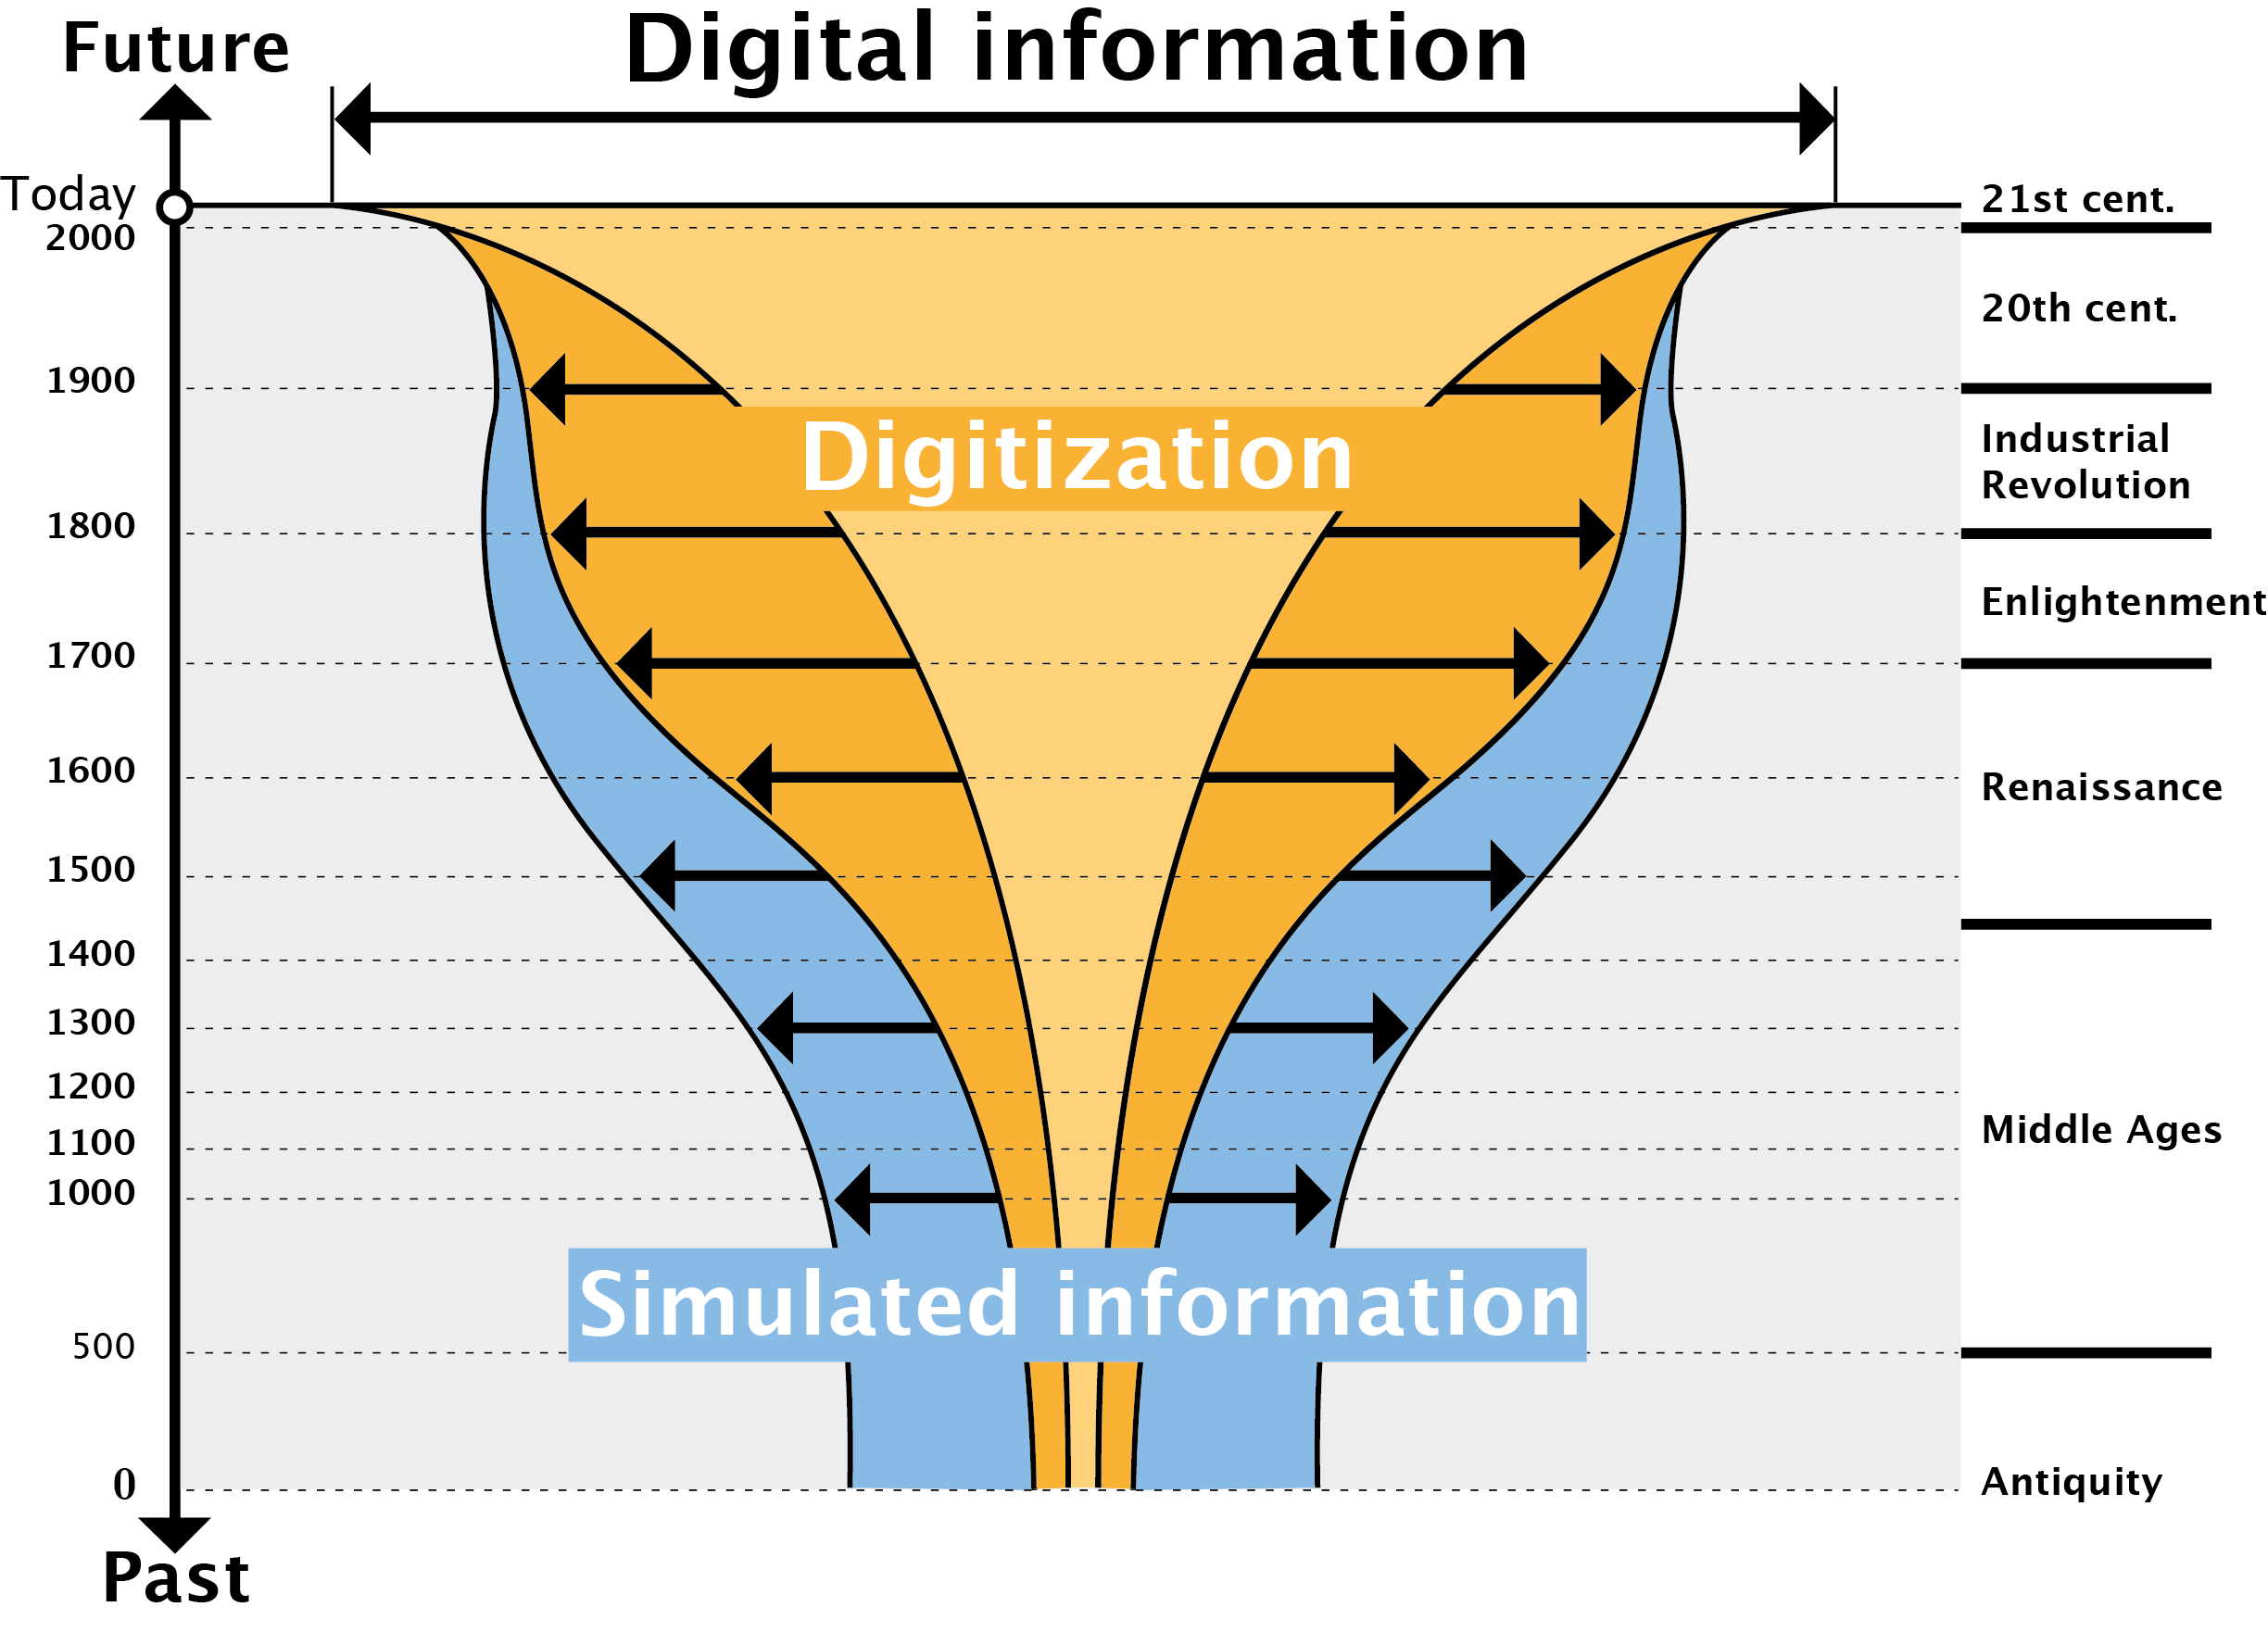
\includegraphics[width=\linewidth]{champignonKaplan.png}
 \legend{Legendary table}
  \end{sidecaption}
\end{figure}

Mais ce serait une erreur que de limiter l'application de ces nouveaux outils aux seuls stockages numériques récents, et ne pas citer l'importance du volume de connaissances accumulées ces derniers siècles par certaines sciences sociales telles que l'archéologie ou encore la géographie. Les lacunes dans l'information sont depuis longtemps une problématique récurrente pour de nombreuses disciplines en Sciences Humaines et Sociales. L'outil computationnel a permis dès lors qu'il a été disponible d'envisager de combler ces lacunes efficacement. Voir la figure ci dessous \ref{fig:I_Champi} \footnote{Voir l'article sur son blog \href{http://fkaplan.wordpress.com/2013/03/14/lancement-de-la-venice-time-machine/}{@FrédéricKaplan}}

%\begin{figure}[tb]
%\raggedright
%\begin{sidecaption}{This is a subcaption just for illustration purposes. This is a subcaption just for illustration purposes. 
%Champignon Informationnel de Frédéric Kaplan. Page number is \LARGE\textbf{\thepage}}[fig:test]
%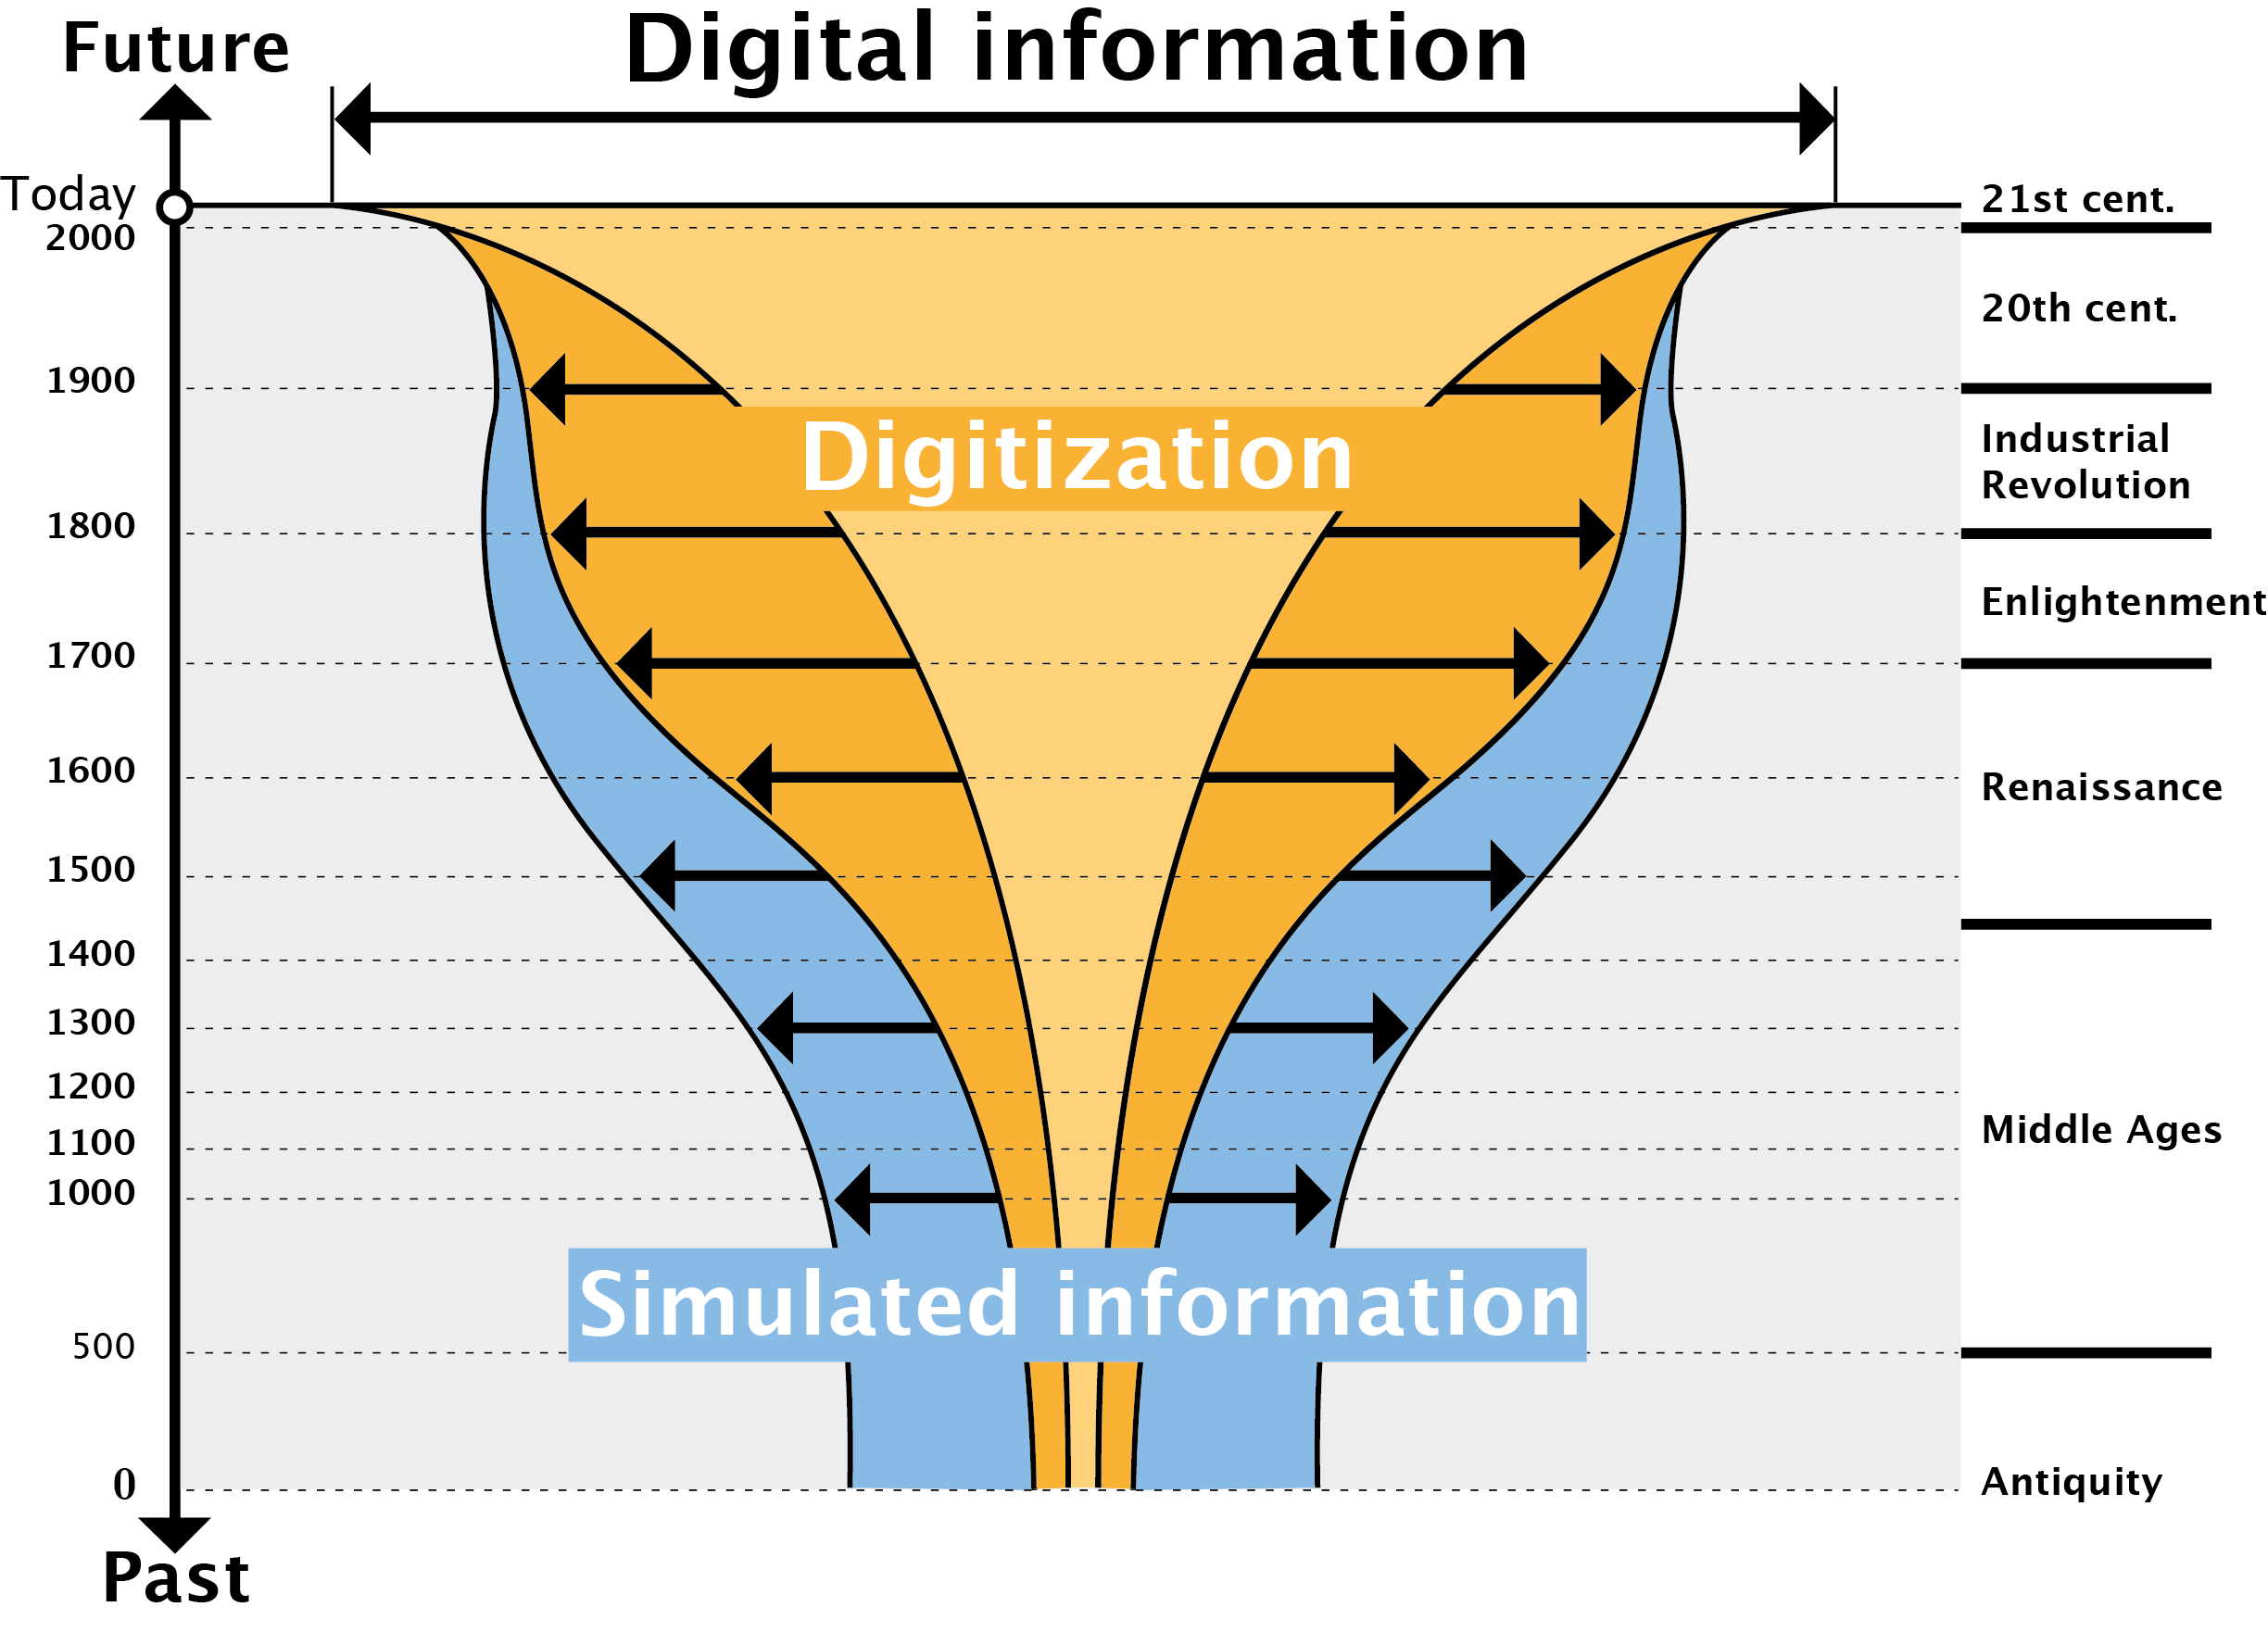
\includegraphics[width=\linewidth]{champignonKaplan.png}
%\end{sidecaption}
%\end{figure}

La classification automatique des données par l'ordinateur mais aussi la construction de modèles et leur simulation (au sens d'abord mathématique et parfois algorithmique du terme) apparaît rapidement comme un enjeu pour la géographie. La simulation apparaît comme un outil de construction de connaissance absolument naturel et nécessaire pour confronter et construire les théories en rapport avec ces données \autocite{Kao1963, Hagerstrand1967b}. L'image de cette communauté inter-disciplinaire agitant et confrontant ses problématiques méthodologiques, techniques, théoriques dans un but de progression commun, fait écho à des revendications plus récentes \footnote{On pensera notamment à la communauté ABM inter-disciplinaire qui gravite autour de la revue JASSS fondée en  1990}. En réalité cet esprit de partage tient d'une \enquote{volonté commune} qui apparaît quasiment avec l'apparition et la démocratisation des techniques de simulation. C'est ainsi que l'on trouve trace des efforts de cette communauté de chercheurs dans plusieurs ouvrages tels que \autocite{Beshers1965,Naylor1966,Dutton1971,Guetzkow1962,Guetzkow1972}.

Une citation d'un météorologiste du MIT, tout à fait remarquable par sa lucidité, anticipe ce qui sera le principal argument de l'emploi de la simulation en sciences humaines, à savoir un substitut à l'expérimentation \foreignquote{english}{I have argued that in the near future the social science will remain largely empirical and that simulation can serve as a device for making experiments \textbf{in vitro}. I think that this use is more important, at this time, than the massive making of models and that the principal contribution of simulation lies in the direction of intelligent, vivacious empiricism} \autocite{Fleisher1965}

%Forrester1969 à ce sujet "In the social sciences failure to understand systems is often blamed on inadequate data... The barrier is deficiency in the existing theory of structure." \autocite[355]{Batty1976}

\subsection{Les conditions d'apparition de la simulation dans les différentes sciences sociales }
\label{sec:apparition_simu_science_sociales}

\subsubsection{Bref rappel autour des définitions de modèles et de simulations}
\label{ssec:rapell_termes_generiques}

Nous apportons ici une petite digression afin de préciser quelle acception de la simulation nous souhaitons mettre en oeuvre dans notre thèse.

\paragraph{Définitions générales du terme \enquote{modèle}}

\textcite{Varenne2013} ont entrepris une classification de la richesse historique associée aux termes de modèle et de simulation.

La première définition généraliste et aussi la plus couramment encore rencontrée dans la littérature est probablement celle de Marvin Minsky établie en 1965 \autocite{Varenne2008} \autocite[15]{Varenne2013}  : \enquote{ Pour un observateur B, un objet A* est un modèle d’un objet A, dans la mesure où B peut utiliser A* pour répondre à des questions qui l’intéressent au sujet de A } \autocite{Minsky1965}

A partir de cette définition très formelle, Franck Varenne \autocite{Varenne2008} relève dans une analyse plus moderne du terme les cinq points suivants : 
\begin{enumerate}
  \item Le modèle n'est pas nécessairement une représentation
  \item Le modèle doit son existence à l'existence d'un observateur subjectif, et d'un questionnement lui aussi subjectif
  \item Le modèle est un objet qui a une vie propre, une existence autonome
  \item L'existence du modèle est justifiée par l'existence d'une \enquote{fonction de facilitation}
  \item Cette caractérisation minimale permet l'établissement d'une typologie
\end{enumerate}

Franck Varenne propose dans des travaux plus récents \autocite{Varenne2013} d'associer à cette définition les travaux de Mary S. Morgan et Margaret Morrison qui replacent et caractérisent le rôle du modèle dans une enquête de connaissance par sa fonction de médiation (point 4 de la liste), une façon de faire écho à la problématique motivant la construction de modèles établie dans la définition de Minsky.

Un modèle est ainsi défini comme \enquote{un objet médiateur qui a pour fonction de faciliter une opération cognitive dans le cadre d'un questionnement orienté}, opération cognitive qui peut être de cognition pratique (manipulation, savoir-faire, apprentissage de gestes, de techniques, de conduites, etc.) ou théorique (récolte de données, formulation d'hypothèses, hypothèses de mécanismes théoriques, etc.) \autocite{Varenne2013}

Les travaux actuels de \textcite{Varenne2008, Varenne2013} dénombrent pas moins de cinq familles pour un total de vingt grandes fonctions, ce qui permet de situer efficacement la ou les problématiques - rien n’empêche les fonctions de se recouper - qui motivent la construction d'un modèle. 

Nous verrons dans la section \ref{ssec:revol_modele} que les géographes modélisateurs ont mis dans leur définition davantage l'accent sur le rôle et les résultats attendus des modèles, plutôt que sur ces aspects formels.

\paragraph{Définition générale du terme \enquote{simulation}}

Le terme \enquote{simulation}, tout comme le terme \enquote{modèle}, est porteur d'une polysémie qui remonte aux alentours de l'accélération de sa diffusion en 1960 \footnote{ \textcite[343-350]{Morgan2004} propose une analyse intéressante de la diversité d’acception pouvant sous tendre l'emploi du terme \enquote{simulation} en se basant sur l'état de l'art réalisé par \textcite{Shubik1960a} en 1960, mais on peut aussi citer des sources plus directes comme les rapports fait par les instituts scientifiques militaires proche de l'OR : \foreignquote{english}{ The term \enquote{simulation} has recently become very popular, and probably somewhat overworked. There are many and sundry definitions of simulation, and a review and study of some of these should help in gaining a better perspective of the broad spectrum of simulation.} \autocite{Harman1961}}, mais nous retenons ici simplement les acceptions qui concernent la simulation computationnelle.

Bien que la simulation apparaisse sous sa première forme computationnelle dans la technique de Monte-Carlo et les travaux de Von Neumann et Ulman \autocite{Eckhardt1987}, il faut attendre les années 1960 et les avancées techniques nécessaires pour que son utilisation semble utile. L'historienne en économie \textcite{Morgan2004} estime que le mot se diffuse vraiment dans la communauté inter-disciplinaire, et en économie, aux alentours de 1960. Elle souligne le rôle central de Martin Shubik, un des pères de la théorie des jeux \footnote{voir sa \href{http://blogs.library.duke.edu/rubenstein/2012/12/18/the-martin-shubik-papers-from-early-game-theory-to-the-strategic-analysis-of-war/}{@Biographie}} dans la construction de ce débat autour de la notion \footnote{Shubick est aussi présent à un des tout premiers symposiums sur le sujet organisés par \textit{American Economic Review} \autocite{Shubik1960b}, où il retrouve d'autres pionniers de son époque, comme \textcite{Orcutt1960}, et Clarkson aidé de Simon \autocite{Clarkson1960}}, comme celui qui a servi à la fois d'intermédiaire important dans la rencontre entre les différents acteurs de l'économie expérimentale et de l'informatique, mais aussi comme celui tout aussi important de prospecteur au travers des vastes études bibliographiques qu'il a réalisées sur le sujet \autocite{Shubik1960a, Shubik1972} \autocite{Morgan2004}.

Par la suite d'autres conférences et ouvrages vont proposer de délimiter, toujours dans une construction inter-disciplinaire, cet objet \enquote{simulation}, comme on peut le voir dans \autocite{Guetzkow1962, Borko1962, Guetzkow1972, Dutton1971}. La simulation computationnelle est rapidement reconnue par les disciplines en sciences sociales ou les sciences du comportement comme un outil important pour la construction et l'extension de théories (\textit{theory-building} ou \textit{model-building} selon la fonction définie pour le modèle), de par sa capacité à manipuler certes des symboles mathématiques, mais aussi des symboles de plus haut niveau d'abstraction, propre à l'établissement de règle \autocite[924-925]{Clarkson1960}. Dans notre étude les modèles de simulation seront évoqués dans leur dimensions avant tout numérique ou algorithmique (cf. dirigés par des règles) \autocite[36-38]{Varenne2013}.

\subsubsection{La simulation vue comme laboratoire virtuel d'expérimentation, une analogie ancienne}
\label{ssec:labo_virtuelle}

Parmi la vingtaine de fonctions épistémiques recensées par \textcite[14-23]{Varenne2013} motivant la construction de modèles de simulation, la caractéristique la plus souvent exprimée pour l'époque en sciences sociales est sûrement cette capacité à pouvoir \enquote{expérimenter} sur les modèles en mobilisant des processus et des interactions sélectionnés et animés dans le cadre d'une dynamique, d'un temps mimant celui des systèmes cibles \footnote{Plusieurs auteurs, comme \autocite[462]{Gullahorn1965}, \autocite[296]{Doran1970}, \autocite[294-295]{Batty1976} semblent faire référence implicite ou explicite à cette action de \enquote{plonger le modèle dans le temps}. Hors \autocite[31]{Varenne2013} indique que cette dénotation se rapporte principalement au temps du système cible, et non pas au temps du modèle, qui peut être simulé autrement (en usant par exemple d'un tirage probabiliste). Cette référence n'est donc pas un marqueur permettant de caractériser en elle-même la notion de \enquote{simulation de modèle}}, et cela même dans des conditions difficiles caractérisées par l'absence ou l'inconsistance des données, les expérimentations réelles impossibles ou difficiles, etc. mais pas seulement, car la simulation de modèles a aussi vocation à simplifier certaines simulations physiques coûteuses, ou trop limitées dans l'expression de nouvelles hypothèses. Ce lien entre simulation et expérimentation, complexe du fait de la relation entretenue entre le modèle et la réalité, est aussi ancien que la technique elle-même, Von Neumann affirmant dès le départ sa volonté de remplacer par des simulations sur ordinateur certaines techniques coûteuses de simulation physique \autocite[15]{Winsberg2013}.

\Anotecontent{laboVirtuel}{Les récentes et au moins tout aussi récurrentes critiques sur l'apport d'une telle expérimentation dans les sciences sociales montrent qu'il est intéressant de développer quels sont véritablement ces points de similitudes et de divergences entre l'expérimentation physique et virtuelle, ne serait ce que pour construire une argumentation lisible à destination des nouveaux modélisateurs. Des sociologues des sciences comme Bruno Latour ou Ian Hacking ont développé ces vingt dernières années une véritable épistémologie des pratiques de laboratoire centrées autour de la démarche expérimentale, des réflexions qu'il nous faut prendre absolument prendre en compte pour toute analyse qui se voudrait plus poussée sur cette notion, comme en témoignent les travaux récents des épistémologues spécialisé dans la simulation comme Winsberg, ou \textcite[204]{Varenne2012}}

Régulièrement employée dans la littérature, cette fonction d’expérimentation revient également sous la forme de \enquote{laboratoire virtuel}, un terme qui prend selon les époques des teintes légèrement différentes, et cela quelles que soient les techniques sous-jacentes de support à la simulation des modèles.\Anote{laboVirtuel}

Cette analogie ancienne entre simulation et laboratoire virtuel est illustrative d'une réalité dont on aurait bien du mal à nier l'existence tant celle ci est persistante dans cette littérature. Parfois le terme est invoqué directement, parfois il est implicite au discours présenté. Pour ne citer que quelques auteurs pionniers dans l'historique de la notion, les premier ouvrages collectifs en simulation et science sociale de \textcite{Borko1962, Guetzkow1962, Guetzkow1972}; les rapports et états de l'art des instituts scientifiques militaires américains \autocite{Harman1961}, \footnote{La légende veut que l'idée d'appliquer la simulation aux \textit{Behavioral Science} viendrait d'un déjeuner entre Guetzkow et des physiciens nucléaire lors de son séjour au Carnegie, pour en savoir plus : \href{http://www.hawaii.edu/intlrel/pols635f/Guetzkow/hg.html}{@Harold} } \footnote{L'ouvrage de 1962, difficile à trouver, contient des re-publications de publications inédites dans plusieurs disciplines : Orcutt en économie \foreignquote{english}{Simulation of economic systems}, Coleman en sociologie \foreignquote{english}{Analysis of social structures and simulation of social processes with electronic computers}, Abelson en psychologie et science politique \foreignquote{english}{Simulmatics project}, Hovland en psychologie sociale avec \foreignquote{english}{Computer simulation of thinking} } et les travaux de Herbert Simon et Alan Newell \autocite{Newell1961}; et de façon plus localisé, en économie \textcite[915]{Shubik1960b}, en psychologie sociale \textcite{Abelson1968} \footnote{Un auteur connu aussi pour avoir échangé aussi avec \textcite{Boudon1967} sur la simulation à la même période, voir  \textcite{Padioleau1969}}, \textcite{Fleisher1965} météorologue, le couple d'Anthropologues/sociologues du comportement \textcite{Gullahorn1965}, l'archéologue anthropologue et informaticien \textcite{Doran1970}, la physicienne biostatisticienne et démographe \textcite{Sheps1971}, l'informaticien \textcite[3-4]{Forrester1971}, l'économiste informaticien \textcite{Naylor1966}, le professeur de science régionale \textcite[271]{Harris1966}, l'urbaniste \textcite[295]{Batty1976} sans oublier plus récemment \textcite{Epstein1996}, l'écologue \textcite{Grimm2006}, et encore sûrement bien d'autres auteurs. Une longue liste qui témoigne de l'intérêt pour cet outil bien au delà d'un simple critère de démarcation disciplinaire, technique, ou encore temporel; une hypothèse que nous allons développer par la suite.

\subsubsection{Un engouement pour la simulation qui touche l'ensemble des sciences sociales}
\label{ssec:engouement_sciencesociale}

Cet engouement pour la simulation de modèles touche toute les sciences sociales ou presque. Nous dressons dans les paragraphes qui suivent une brève énumération des travaux qui en témoignent pour la période 1950-1970.

Suite au mouvement Cybernétique, à la convergence des travaux sur l'intelligence artificielle et les sciences cognitives, les premiers travaux qui visent la démonstration de la faisabilité de la simulation dans les sciences sociales viennent de Newell, Shaw, et Simon à la fin des années 1950 \autocite{Gullahorn1965} \footnote{Avec plusieurs tentatives pour la construction d'une machine universelle de résolution de problème (\foreignquote{english}{Logic Theorist program} en 1957 et \foreignquote{english}{General Problem Solver} en 1959). Ce programme s'avère également être la première pierre posée de l'intelligence artificielle, en formation à l'intersection de la naissance encore récente des sciences cognitives et de l'informatique. Cette machine est conçue pour mimer les capacités de résolution de l'esprit humain, et permet enfin d'exprimer et de questionner les théories comportementales dans un langage informatique alors plus précis et moins ambigu que le langage naturel. Le programme est ainsi capable de résoudre des problèmes aussi différents que de jouer aux échecs, de résoudre des problèmes mathématiques, ou de retrouver des motifs dans des données.} A ces travaux s'ajoutent ceux, en psychologie linguistique de l'équipe gravitant autour de \textcite[280-416]{Borko1962}, en psychologie des comportements sociaux de \textcite{Hovland1960}, d'\textcite{Abelson1961, Abelson1968} ou du couple \autocite{Gullahorn1965a} qui utilisent la simulation de modèle pour formuler, vérifier des théories sur la psychologie des individus et les modalités de leurs interactions avec les autres dans diverses situations \footnote{Les applications sont menées à des échelles très diverses, ainsi alors que le modèle Homonculus développé par le couple Gullahorn tente de mieux comprendre les stratégies de résolution de conflits avec la programmation de comportements au niveau individuel \autocite{Gullahorn1965}, le projet \textit{Simulmatics} mené par \textcite{Abelson1961} vise quand à lui l'étude du comportement de groupes d'électeurs en cas de conflit d'opinion (ou \foreignquote{cross-pressure}) pour tenter en fonction d'un échantillon de population d'analyser l'impact de stratégies politiques, une demande de J.F.Kennedy pour la campagne de 1960 aux États-Unis}, ce que \textcite{Ostrom1988} appellera \foreignquote{latin}{a posteriori} les \foreignquote{english}{complex human processes}.

%La formation d’ingénieur de Coleman l’amène à prendre comme modèle un physicien : « My real hero is not Isaac Newton, but James Clerk Maxwell. He took Newtonian theory and developped from it a theory of gases, the Maxwell-Boltzmann distribution law of molecular velocities. I was fascinated by Maxwell because he was also concerned with the micro-macro problem. He had a very simple and neat theoretical framework of dimensionless molecules of any gas acting according to the law of motion, each with a certain mass and velocity. And from this he constructed a theory of gas. » (Coleman dans Swedberg, 1990, pp. 55-56).

En \textbf{sociologie}, la simulation émerge dans les années 1960-1970 selon \textcite[50]{Manzo2005}, sous l'impulsion de pionniers dans la sociologie mathématique comme \textcite{Boudon1967} en France \footnote{Selon \textcite[61]{Manzo2005}, Boudon a très tôt supporter l'idée des modèles de simulation comme support à l'explication, comme il témoigne à propos de ces écrits des années 60-80 : \enquote{À ce moment, j’avais publié divers écrits sur l’individualisme méthodologique, la théorie de l’action, la rationalité et les \enquote{modèles générateurs}. Mes travaux sur l’éducation m’avaient en effet convaincu que ni l’analyse multivariée ni les méthodes statistiques d’\enquote{analyse des données} ne permettaient d’expliquer les régularités statistiques qui sont le pain quotidien du sociologue : il fallait tenter plutôt de les engendrer à partir d’hypothèses sur les logiques de comportement des acteurs.} \autocite[391]{Boudon2003}}, ou James Samuel Coleman aux Etats-Unis \footnote{C'est à l'université de Columbia sous la direction du sociologue Robert Merton et du mathematicien-sociologue Paul Lazarsfeld, des acteurs influents dans l'application des méthodes quantitatives à la sociologie \autocite{Lazarsfeld1954} aux États-Unis mais également en France (il collabore avec Boudon sur plusieurs projets, d'enseignements et de publications) et à l'international \autocite{Lecuyer2002}, que James Coleman publie en 1964 \textit{Introduction to Mathematical Sociology} \autocite{Coleman1964}, un ouvrage devenu une référence en sociologie quantitative dont on peut lire un résumé élogieux dans la \textit{Revue francaise de Sociologie} réalisé par \textcite{Boudon1966} en 1966.} et de simulation, celui-ci considérant cette dernière {[...] as a half-way point between verbal speculative theory and formal theory, aiding in the development of such theory through concretizing the functioning of \foreignquote{english}{social processes}. \autocite[36]{Guetzkow1972}}.

Celui-ci travaille sur des simulations liées à ses recherches sur l'éducation au début des années 1960 aux États-Unis, dont il a déjà publié des travaux dans l'ouvrage inter-disciplinaire de \textcite{Guetzkow1962} en 1962, et qu'il publie ensuite \autocite{Coleman1965} dans une des premières revues abordant la méthode de simulation en sociologie, un numéro spécial des \textit{Archives Européennes de Sociologie} introduit par \textcite{Boudon1965} en 1965. Dans ce  numéro figure également une des premières traductions de la simulation de diffusion d'Hägerstrand \autocite{Hagerstrand1965} utilisant la technique de Monte-Carlo, un modèle qui recoupe les préoccupations du vaste courant inter-disciplinaire dit des SNA (Social Network Analysis) \autocite{Bernard2005}, qui touche tout autant aux structures de parenté (voir le paragraphe suivant pour des références en Anthropologie), qu'à la géographie (Hägerstrand à Lünd), ou à la sociométrie (modèle du sociologue mathématicien Coleman \textcite{Coleman1957}, mais également modèle de \textcite{Rapoport1961}, un biomathématicien de Chicago et confondateur avec Boulding, Gerard et Von Bertalanffy de la société pour l'étude des systèmes généraux, ou GST) \footnote{Une analyse croisée entre des modèles de différentes disciplines sur la diffusion des innovations, contenant notamment les modèles d'Hägerstrand et de Rapoport a été publiée en 1968 dans la revue \textit{Lund Studies in Geography} par \textcite{Brown1968}}. Du point de vue français, outre l'analyse de Boudon sur ce sujet dans le numéro spécial de 1965, on trouve également une revue de ces mêmes avancées en simulation du côté de la sociologie politique (qui recoupe la psychologie sociale américaine), un état de l'art réalisé par \textcite{Padioleau1969} dans la \textit{Revue francaise de sociologie} en 1969.

\Anotecontent{archeo_stat}{Des transferts parfois étonnants en provenance d'autres disciplines, comme le montre cette citation : \foreignquote{english}{Similar trends are apparent in allied subjects such as anthropology and social geography. In particular, location analysis has influenced archaeologists, with its emphasis on the study of all aspects of a population and its environment, and on the use of quantitative methods and models (Haggett 1963)} \autocite{Doran1970}}

\Anotecontent{archeo_systemique}{Une analyse a posteriori confirme l'apport de la systémique dans la construction des modèles de simulation, comme en témoigne \textcite[5]{Lake2013} et de façon plus précoce \textcite{Aldenderfer1998} en 1988. \foreignquote{english}{One of the theoretical hallmarks of the \textit{New Archaeology} was the systems approach \autocite{Aldenderfer1991}, and a result of its adoption was the use of computer simulation to model whole societies or significant portions of them.}}

\Anotecontent{whallon_simulation}{\foreigntextquote{english}[Whallon1972, 38]{The techniques and procedures of computer simulation so closely parallel the current thinking and processes of model-building of many archaeologists that the lateness and limits of their application are surprising.}}

%% FIXME ORTHOGRAPHE
En archéologie, dans la très claire retrospective historique faite par Gary Lock en 2003\autocite{Lock2003} sur l'histoire de l'archéologie computationelle, l'auteur s'attache à bien séparer au moins deux sinon trois époques aux méthodologies et aux outils différents. En adoptant une posture un peu simplificatrice on peut donc affirmer que si l'archéologie pre-années 1960 se base principalement sur la récolte de données empiriques et la mise en exergue de pattern dans ces même données pour générer la plupart de ces explications, une rupture dans la discipline se dessine dès les années 1960-70 avec l'avénement d'un courant d'archéologie proclamant une \enquote{ new archeology} (ou \emph{processualism}). Rejettant un empirisme beaucoup trop subjectif, celle ci vante le retour à la seule \enquote{ Méthode Scientifique } pour générer des explications. 

\Anotecontent{wilcock_stat}{On trouve un récit plus détaillé de l'arrivée des méthodes statistiques en archéologie dans la publication de \autocite{Wilcock1997}}

\Anotecontent{caa}{Il est intéressant de noter que ces quelques archéologues pionniers en informatique ont très vite créés leur propres canaux de diffusion en angleterre. Si de multiples conférences pour le développement des aspects computationels en archéologie existent à la charnière 1960-1970 (Rome, New-York, Marseille) \autocite{Wilcock1997}, ce n'est qu'en 1973 que se forme sous le patronage de quelques chercheurs anglais la première \foreignquote{english}{Computer Applications and Quantitative Methods in Archaeology Conference} \href{http://caaconference.org/about/}{@CAA}. Celle-ci se tient sa première édition à Birmingham, et deviendra par la suite en 1992 une conférence à portée internationale. La particularité de cette conférence, qui existe toujours, est son inter-disciplinarité; le comité d'organisation militant toujours pour la rencontre et le dialogue entre  archéologues, mathématiciens et informaticiens. A l'ocasion des 40 ans de la conférence en 2012, le projet \foreignquote{english}{Personnal-Histories Project} à permis la collecte et la mise à disposition de témoignages vidéo des pionniers sur le site de \href{http://www.sms.cam.ac.uk/collection/750864}{@Cambridge}}

Si la critique de 1962 opéré par \textcite{Binford1962} cristalise pour beaucoup cette rupture, 1968 est également considéré comme une année particulièrement importante pour la structuration de ce courant dans la discipline. L'avénement de plusieurs publications phares vient souligner l'émergence progressive dans les années 1960-70 de nouveaux outils \Anote{caa}, à la fois computationels comme les statistiques \Anote{wilcock_stat} ou la simulation \autocite{Clarke1968} , ou plus conceptuels avec l'ancrage de la \foreignquote{english}{New Archeology} dans la pensée systémique \autocites{Clarke1968, Flannery1968, Binford1968} \Anote{archeo_systemique}. Des avancées qui fournissent un véritable support à ce changement des pratiques dans la discipline.

\Anotecontent{doran_intuition}{\foreignquote{english}{There has now been a wide variety of experiments involving computer processing of archaeological data. Clarke (1968) describes many of them, and another valuable source is Cowgill (1967). I do not propose to discuss these experiments here, important though they are. [...] In this final section I shall briefly present the computer in what seems to me to be a much more promising and interesting role, which has as yet received rather little attention from archaeologists, even though in some ways it can be regarded as the practical equivalent of systems theory. I mean the use of a computer to construct and test a \enquote{simulation} of some complex system evolving in time. [...] Indeed, one of the great advantages of using a computer program to simulate evolving systems is that a much wider range of possibilities can be accommodated than can be expressed mathematically.} \autocite{Doran1970}}

Si \textcite{Binford1968} représente le point de vue américain, Clarke présente en angleterre et à la même période (\textcite{Clarke1968} est édité en 1968 par Binford) un point de vue un peu différent sur la New-Archeology \autocite{Binford1983}. Clarke est en effet sous l'influence des idées animant le campus de Cambridge, un haut lieu de changement ayant déjà accueilli une autre révolution, celle de la \textit{New-Geography} \Anote{archeo_stat}. C'est dans cet environnement que Clarke publie en 1968 un premier livre \foreignquote{english}{Analytical Archeology} qui démontre le potentiel que pourrait avoir les statistiques spatiales, les modèles et la simulation stochastique en archéologie \autocites{Clarke1968, Clarke1972} (ce dernier meurt jeune en 1976). Il est accompagné dans ses travaux par l'expertise, la volonté et les intuitions pionnières \Anote{doran_intuition} de James Doran \autocite{Doran1970} qui écrit également avec Hodson en 1975 l'ouvrage devenu référence \foreignquote{english}{Mathematics and Computers in Archaeology} \autocite{Doran1975} faisant état des travaux utilisant les toutes dernières techniques computationelles à la fois en traitement de données, et en simulation (Chaîne de Markov, Monte-Carlo, langage pour la simulation Dynamo, GPSS, etc.)

Ce militantisme qui semble recevoir un écho positif tout au long des années 1970 \footnote{On pourra trouver plus d'informations sur les premiers travaux dans les ouvrages cités précédemments, et via des retrospéctive plus récente comme celle de \autocite{Kohler2011}, ou \autocite{Lake2013}}, certains auteurs comme \textcite[38]{Whallon1972} n'hésitant pas à définir\Anote{whallon_simulation} la simulation comme un prolongement naturel à la pratique existante de construction des modèles. Cette mise en oeuvre de programmes pionniers se poursuit avec une diversification dans les usages jusqu'au début des années 80 et constitue une première phase d'appréhension de la simulation, plus qu'une adoption massive par la discipline. \autocite{Lake2013}

% VOir aussi Mathematics and Computers in Archaeology doran 1975, partie sur la simulation cf http://books.google.fr/books?id=ZAPvXcnz0kkC&pg=PA369&lpg=PA369&dq=The+computer+in+archaeology:+A+critical+survey+whallon&source=bl&ots=6et-F8jHab&sig=gQWgTIHRuO2ICqMJtrRdGovo9gs&hl=fr&sa=X&ei=OskxU5W5Nen20gW0_4DIDA&ved=0CGUQ6AEwBQ#v=onepage&q=whallon&f=false

%\autocite{Clarke1987}

A la croisée de plusieurs disciplines, sociologie, anthropologie et géographie on trouve les modèles de variation de population, ou modèles démographiques dont les hypothèses sont amenées à varier selon des facteurs biologiques, économiques, spatiaux faisant souvent appel à une dynamique des interactions humaines impossible à expérimenter dans la réalité. \footnote {\foreignquote{english}{To understand how changes in the size and composition of human populations occur, it is essential to study the determinants of these changes and the interrelations among them. The impossibility of investigating these relationships experimentally stimulates the formulation of models, as a means of enhancing our understanding of the process.} \autocite{Sheps1971}} Dans cette branche se côtoient donc macro-simulation, micro-simulation et modèle analytique hérités des premiers démographes mathématiciens, comme le plus connu d'entre eux, Lotka dont les premières publications sur le sujet datent de 1907 \autocite[355]{Veron2009}.

%%FIXE CLEMENTINE : c’est intéressant, que la plupart des travaux pionniers que tu cites  apparaissent dans les urban studies.  Est-ce que c’est la ville qui est si complexe ou une dépendance au chemin des méthodes dans les champs d’études ? ou parce que urban studies est particulièrement interdisciplianaire que ça a dépasser les barrières des affiliations disciplinaires ?

Les modèles TRIM, puis DYNASIM (entre 69 et 75) développés par Orcutt et son équipe à l'\foreignquote{english}{Urban Institute} sont pionniers \autocite{Orcutt1957, Orcutt1960, Orcutt1976}, et inspirent différents modèles dynamiques en démographie avec les travaux de \textcite{Perrin1964}, \textcite{Sheps1971}, et \textcite{Ridley1966} avec REPSIM aux États-Unis,  \textcite{Hyrenius1964} en Suède, \textcite{Horvitz1971} avec POPSIM, ou encore SOCSIM basé sur les travaux en anthropologie de \textcite{Gilbert1966}, qui viennent compléter efficacement les modèles analytiques inspirés des travaux de Lotka \autocite{Sheps1971}, père entre autre de la démographie mathématique moderne. Coïncidence de l'histoire, ou inspiration commune, Hägerstrand apportera de façon parallèle en géographie, et dans la même décennie \autocite{Hagerstrand1952, Hagerstrand1967}, une vision micro similaire, à cela près qu'elle y ajoute un ancrage spatial des individus.

Dans le cas de l'anthropologie, qui partage un tronc commun avec nombre de problématiques en archéologie, et en psychologie, on retiendra le manuel édité par \textcite{Hymes1965} retranscrivant une conférence de 1962. Celui-ci contient deux articles importants pour la discipline, celui de \textcite{Gullahorn1965} et celui complémentaire de \textcite{Hays1965}. L'intégration de la simulation dans l'arsenal méthodologique prend part selon \textcite[274]{Bentley2009} d'un mouvement ayant pour objectif de mieux comprendre les contraintes sociales et culturelles dans les processus démographiques en général. Dans ce cadre par exemple de l'étude de la parenté ou \foreignquote{english}{kinship}, l'application de la simulation donne lieu à plusieurs expériences pionnières \autocite{Dyke1981} en simulation comme celle de \textcite{Kunstadter1963}, mais aussi de \textcite{Gilbert1966}. Cet engouement continuera dans les années 1970 \autocite{Read1999} avec des simulations mettant en œuvre des processus stochastiques dynamiques comme par exemple dans les travaux de \textcite{Howell1978} et \textcite{Thomas1973}.

%\autocite{Costopoulos2007} . %Antony Wallace également, levy strauss 1955: les mathématiques de l'homme...

%En utilisant la simulation non pas comme un solveur d'équation mais en utilisant la puissance des opérateurs symboliques à sa disposition pour la mise en temporalités de systèmes d'interaction dans des sociétés passées, Doran décrit une vision de la simulation qui n'est pas sans rapeller le multi-agent d'aujourd'hui. Une conception de la simulation reprise et concrétisée par DH Thomas en 1972.\footnote{La discussion sur  \href{www.jiscmail.ac.uk/cgi-bin/webadmin?A2=ind04\&L=simsoc\&F=\&S=\&P=39083} {@SimSOC}} 


% http://books.google.fr/books?id=G8sA95bz5pwC&pg=PA143&lpg=PA143&dq=%22Social+Physics%22+stewart+cybernetics&source=bl&ots=FsOC2mqHvr&sig=cS914G7pelGvgG6bG32fKsmWWPc&hl=fr&sa=X&ei=yTRAU5m7OIOH0AXwtYEY&ved=0CDsQ6AEwAQ#v=onepage&q=%22Social%20Physics%22%20stewart%20cybernetics&f=false
% "Social Physics" stewart cybernetics
% http://www.eoht.info/page/Princeton+Department+of+Social+Physics
% http://books.google.fr/books?id=F84mS2nnjWsC&pg=PA105&lpg=PA105&dq=geographer+reino+ajo&source=bl&ots=buVSBElr7Y&sig=_NXU0Py2goM2c6fVi1To3dUwqHQ&hl=fr&sa=X&ei=0DBAU_niJqrO0AWk44CwCw&ved=0CG8Q6AEwBw#v=onepage&q=geographer%20reino%20ajo&f=false
% http://www.persee.fr/web/revues/home/prescript/article/ingeo_0020-0093_1957_num_21_5_6491_t1_0223_0000_5#
% http://www.eoht.info/page/Social+physics
% Contributions to "social Physics" reino ajo
% Stewart, J.Q. "The Development of Social Physics"

\subsection{Les premiers modèles de simulation en géographie}
\label{sec:premier_modele_geo}

\subsubsection{Une \enquote{révolution quantitative} au cœur de multiples convergences}
\label{ssec:revol_quanti}

L'apparition et la diffusion de ces techniques quantitatives n'est pas le résultat d'une convergence unique, mais bien d'une succession de moments dont la fréquence et l'étalement temporel est difficile à cerner et empêche sur ce sujet toute exhaustivité. 

On retiendra toutefois plusieurs grands facteurs, à la fois généraux, et d'autres plus spécifiques à la géographie, dont certains qui peuvent paraître étonnamment antinomiques. Une convergence qui s'illustre dans la richesse et la diversité des transformations qui touche la discipline géographique entre 1950 et 1970, un constat déjà établi par bien d'autres auteurs \autocite{Varenne2014}

%[28-29]Claval2003
%http://books.google.fr/books?id=s5xjIsejTjkC&pg=PA28&lpg=PA28&dq=h%C3%A4gerstrand+positivism&source=bl&ots=FrIMA95glO&sig=9Knqs1cLfJJefcc30qwsIMDzW-s&hl=fr&sa=X&ei=UMVDU86hJ-mS1AWPmIDoCw&ved=0CC4Q6AEwADgK#v=onepage&q=h%C3%A4gerstrand%20positivism&f=false

\paragraph{L'influence de l'école néo-positiviste}

Le néo-positivisme, néo-empirisme, positivisme logique selon les étiquettes, est un mouvement philosophique important, sinon peut être le plus important, entre les deux guerres. Ce cercle dont on trouve les premières traces dans les années 1908 à Vienne, est organisé autour de grands débats, dont la caractéristique est d'être fréquenté par un grand nombre d'intellectuels, issus de plusieurs disciplines. Tout au long de son évolution caractérisée par différentes phases (avec une apogée durant la troisième phase entre 1928-1934), de multiples courants d'opinions \textcite[126]{Ouelbani2006} vont être amenés à se côtoyer, du fait des débats internes, mais aussi des critiques extérieures au cercle. C'est donc à ce titre que \textcite[11]{Ouelbani2006}, préfère parler de \enquote{programme néo-positiviste} \footnote{Le programme de Carnap tient en quatre points selon Dahms, cités par \textcite{Ouelbani2006} : (i) la réduction de la philosophie à une théorie de la connaissance; (ii) la distinction des sciences, non plus en sciences de la nature et sciences humaines, mais en sciences empiriques et analytiques: (iii) le logicisme comme programme de réduction des sciences analytiques; (iv) le réductionnisme comme programme de réduction des sciences synthétiques ou empiriques.} plutôt que d'un réel courant unifié.

Inspirés des sciences naturelles, et plus particulièrement d'une observation des sciences physiques et mathématiques, les tenants du programme néo-positiviste sont motivés par l'unification des sciences, et pensent l'application d'un tel programme incontournable pour fonder des sciences sociales véritablement \enquote{scientifiques}. \textcite[1-20]{Ouelbani2006}

Les positivistes logiques ont ceci de particulier qu'ils raisonnent sur des démonstrations logiques encapsulant les énoncés observationnels décrits dans une logique formelle qu'ils veulent non ambiguë. Entre empirisme et logicisme, ce programme réductionniste \footnote{Voir la définition du programme donné par Carnap dans la note précédente.} fait porter toute la connaissance sur l'expérience; ce qui mène avec l'aide de l'analyse logique et mathématique à l'élimination de toute métaphysique, et de toute structure a priori (anti-kantien) dans la construction des énoncés d'observation. Ainsi l'inférence déductive se fait seulement sur des énoncés d'observations qui sont \foreignquote{latin}{a posteriori} tout à fait justifiables, et donc mobilisables dans celle-ci seulement si ils cohérents.

Ian Hacking \autocite{Hacking1983} a ,selon Orain \footnote{Voir les notes de \href{http://www.esprit-critique.net/article-12642840.html}{@cours}, dispensés sur le blog \enquote{esprit critique} de Olivier Orain} très bien saisi ce qui fait les axes communs \footnote{Le positivisme peut se définir par quelques idées forces. (1) L’importance accordée à la vérification (ou à une variante comme la falsification) : une proposition n’a de sens que si l’on peut, d’une quelconque manière, établir sa vérité ou sa fausseté. (2) La priorité accordée à l’observation : ce que nous pouvons voir, toucher ou sentir fournit, sauf pour les mathématiques, la matière ou le fondement le plus appréciable de la connaissance. (3) L’opposition à la cause : dans la nature, on ne trouve pas de causalité dépassant ou surpassant la constance avec laquelle des événements d’un certain type sont suivis par des événements d’un autre type. (4) Le rôle mineur joué par l’explication : expliquer peut contribuer à organiser des phénomènes mais le pourquoi reste sans réponse. On peut seulement remarquer que le phénomène se produit régulièrement de telle ou telle manière. (5) Opposition aux entités théoriques : les positivistes ont tendance à être non réalistes parce qu’ils limitent la réalité à ce qui est observable mais aussi parce qu’ils s’opposent à la causalité et se méfient des explications. Leur rejet de la causalité les fait douter de l’existence des électrons simplement parce que ces derniers ont une action causale. Ils soutiennent qu’il s’agit là seulement de régularités constantes entre phénomènes. (6) L’opposition à la métaphysique est finalement le dénominateur commun entre les points (1) à (5) ci-dessus. Propositions invérifiables, entités inobservables, causes, explications profondes, tout cela, dit le positiviste, est objet de métaphysique et doit être abandonné. \autocite[82]{Hacking1983}.} des différentes relectures du terme positivisme. Une parenté qui dans le cas du programme néo-positiviste est difficile à isoler tant l'acceptation par les proches (comme Popper) ou membres du programme (certain préféreront même le terme empirisme logique) est amené à varier, on pourra ainsi se référer à la classification proposée par Hacking pour en savoir plus sur ce sujet. \autocite[81-86]{Hacking1983}

L'apogée du groupe à Vienne est de courte durée, avec les pressions du régime nazi et l'annexion de l'Autriche, le groupe est dissous. De nombreux acteurs du mouvement sont alors contraints à l'exil, et nombreux sont ceux qui vont aux États-Unis. A ce moment-là, ce programme philosophique est alors quasiment inconnu des philosophes pragmatistes américains, mais paradoxalement c'est sur ce nouveau territoire qu'il va trouver un très bon accueil. 

C'est sur cette philosophie pragmatique depuis longtemps installée (Peirce, Dewey) que vient se greffer ce nouveau programme, jusqu'à finalement quasiment l'éclipser. Un transfert que l'on n'imagine pas totalement unilatéral, et il est presque évident que le discours originel viennois tire largement profit d'une philosophie pragmatiste compatible dans ses fondements \footnote{ Ainsi selon \textcite[149]{Ouelbani2006} Carnap aurait été rassuré en 1935, date de son arrivée aux Etats-Unis, \enquote{ [...] de trouver une ambiance philosophique différente,en ce sens que les jeunes philosophes étaient intéréssés par des méthodes scientifiques et logiques}}. C'est ce que \textcite[123]{Wilson1995} affirme en disant que les pragmatistes \foreignquote{english}{[...] had created the conditions in which logical positivism and other analytic philosophies could flourish and ultimately displace them as the dominant voice in mid-century philosophical debates} mais aussi les conditions de son dépassement \foreignquote{english}{Pragmatism, then, not only created the conditions in which logical positivism and analytic philosophy could flourish in the United States, it also contained the seeds of the postanalytic philosophies that have attempted to move beyond [...] }. Ce programme va se diffuser à la fois sur les bancs des universités, mais aussi via les grands instituts scientifiques après guerre qui font publicité de cette science \foreignquote{english}{mainstream}, organisée aux Etats-Unis autour de l'ordinateur. 

La RAND fait partie de ces instituts fondés après guerre, qui approche dès 1947 les sciences sociales \autocite{Rand106}, et n'hésitent pas à mettre en avant par la suite les stars de la philosophie positiviste de l'époque comme Reichenbach \autocite[384-385]{Barnes2011} .

\paragraph{L'apparition de mouvements inter-disciplinaires fédérateurs}

L'apparition de grands mouvements de convergence inter-disciplinaires et leur intérêt pour l'application de nouveaux concepts et techniques aux sciences sociales, dont certains prennent par la suite la forme de paradigme du fait de leur portée d'application : Cybernétique de Wiener, \textit{projet} de la \foreignquote{english}{General System Theory} de Bertalanffy \autocite[9]{Pouvreau2013} s'organise autour de grandes structures de recherches comme le MIT, la RAND, qui favorisent les collaborations par la mise en place d'équipe de travail pluri-disciplinaire.

Parmi les ramifications directes de ces coopérations, on citera par exemple la \enquote{social physics} de Stewart \autocite{Stewart1947}. Du fait des liens développés à l'université de Pennsylvanie, lieu de ses études, et siège de la fondation de la science régionale d'Isard en 1954, Stewart sera amené avec sa rencontre avec Warntz, un géographe atypique qui plonge très tôt dans l'inter-disciplinarité, à publier dans la revue \textit{Regional Sciences} \autocite{Stewart1958}.

Les retombées de ces interactions sur la géographie sont importantes \footnote{ A condition de ne pas oublier qu'une partie de ces concepts existent de façon sous-jacente aux disciplines, ce qui explique parfois leur rapidité d'acceptation. C'est le cas de l'approche systémique développée par la cybernétique quand elle ne fait pas qu'apposer un nom commun sur des concepts déjà étudiés, mais fait alors écho à des révolution méthodologiques en attente d'être activée. \textcite[5]{Batty1976} résume la situation ainsi \foreignquote{english}{The idea of systems being described in terms of structure and behaviour, in terms of input and output, and the notion of purposeful control of such systems in terms of negative and positive feedbacks, appeared to many social scientists an ideal description of their systems of interest and thus the approach has come to be used in more-or-less all of the social sciences}.}, et fournissent tout autant : (i) des concepts généraux en correspondances avec les débats qui animent l'ensemble des sciences : sensibilité aux conditions initiales, équifinalité, bifurcation et catastrophe, boîte noire, rétro-causalité, hiérarchie d'emboîtement, etc.) , (ii) un catalogue d'isomorphisme supplémentaire dont la correspondance reste à évaluer dans notre discipline \autocite{Wilson1969}, (iii)  une méthodologie et une typologie des modèles tirés de la recherche opérationnelle \autocite{Ackoff1962} \footnote{Une discipline proche du projet Bertalanffien en bien des aspects, comme le défend \autocite[801]{Pouvreau2013}} et largement revendiqués par les géographes dans la décennie 1960-70, un constat tiré de la lecture d'états de l'art \autocite{Kohn1970}, ou d'ouvrage phare sur le sujet comme \autocite{Berry1964a, Haggett1965}, (iv) la découverte d'une nouvelle science mathématique de la dynamique en correspondance avec ces nouveaux concepts, accessible soit par un vocabulaire graphique opérationnalisable \autocite{Forrester1961}, soit par des langages de programmation plus traditionnels !

On citera parmi les pionniers d'une exploration volontaire de cette convergence en géographie, Haggett en 1965 \autocite{Haggett1965}, Chorley avec la géomorphologie en 1962 \autocite{Chorley1962}, Berry avec les villes en 1964 \autocite{Berry1964a}

\paragraph{Les influences des \enquote{passeurs de modèles}}

\Anotecontent{footnote_kant}{Edgar Kant (1902-1978) un géographe déjà rompu aux méthodes statistiques en Estonie \autocite{Chabot1937} - où il avait déjà pu appliqué ses méthodes - s'est expatrié d'Allemagne avec dans ses bagages les travaux de Christaller, Lösch, etc. Tuteur d'Hagerstrand il le forme aux différentes méthodes qui vont se répercuter sur ses travaux de thèse.}

Ces influences se sont réalisées à l'échelle internationale par Torsten Hägerstrand, Edgar Kant \Anote{footnote_kant}, Christaller et Lösch \autocite[119]{Berry1970}, ou dans un cadre plus national avec le travail de traduction ou de mise à disposition de textes originaux par les économistes et géographes Lösh, et Isard.

\paragraph{La conjoncture politique favorable}

L'impact de la conjoncture politique et l'importance de grands \textit{Think-Tank} comme la RAND, et du MIT qui remobilisent en sortie de guerre des armées d'ingénieurs alors désoeuvrés sur des missions plus scientifiques. On soulignera à la même période le rôle joué chez les géographes par Ullmann, Harris, Ackerman dans la transformation institutionnelle de la géographie, dont la qualité en tant que corps de métier a pu être remarquée en temps de guerre. Cela se traduit sur la durée par un financement de la marine (\textit{Office Of Naval Research}), qui profite aussi de la nouvelle \textit{Regional Science} fondée par Isard. On trouvera plus d'informations sur ces inter-relations entre instituts après guerre et leur impact sur l'établissement d'une géographie quantitative dans les publications de \textcite{Barnes2006a}.

\subsubsection{D'une révolution quantitative à une révolution des modèles}
\label{ssec:revol_modele}

De cette \enquote{révolution quantitative} aux origines on le voit multiples, certains auteurs préfèrent ne retenir qu'une certaine essence de cette volonté nomothétique. Cette \enquote{révolution des modèles} comme préfère en parler \textcite{Wilson1970, Varenne2014} fait ici écho à cette déferlante de modèles qui apparaissent dans la décennie 1960-1970, et dont on trouve un recensement quasi exhaustif dans plusieurs ouvrages de référence \autocite{Haggett1965,Chorley1967}.

Une fois révélée cette profusion d'approches sous jacentes à l'emploi, parfois confus, d'un même terme, s'ensuit chez les géographes une tentative de classification, de définition de cette pratique de modélisation. Il en ressort des typologies, l'évocation de divers substrats ( analogique, iconique, symbolique ) la plupart du temps empruntés dans les ouvrages de spécialistes alors disponibles. Ainsi les deux sources d'inspirations de \textcite[106]{Berry1963}, \textcite{Haggett1965} sont à ce moment-là des références issues d'un rapprochement avec la Recherche Opérationnelle (RO) \footnote{On en trouve trace également dans des collectes bibliographiques à destination des enseignements comme \autocite{Greer1972}}, une discipline pionnière dont le développement après-guerre oeuvre pour l'application et la diffusion de méthodes numériques en vue de résoudre des problèmes extrêmement diversifiés. On retiendra des auteurs comme \textcite{Ackoff1962} (déjà cité par Ackerman en 1958) ou \textcite{Kemeny1962}

% détails typologies ?
\paragraph{Une autre définition des modèles et de la modélisation}
\label{p:autre_def_modele}

Alors que dans les faits beaucoup de choses ont changé sur le plan des pratiques, des techniques, des institutions, la référence à des définitions datant de 1965 reste après les années 1990 tout à fait acceptable \autocites{Dastes2001b, Antony2013}[295]{Bailly1995}, et sert encore comme base de travail solide pour établir de nouvelles réflexions \autocite{Brunet2000}. 

Comme nous le rappelle dès 1965 Peter Haggett, le modèle est pour les géographes avant tout un construit. En s'appuyant sur la typologie et la réflexion d'Ackoff, il définit ainsi dans \textit{l'analyse spatiale en géographie humaine} : \enquote{En construisant un modèle (\textit{model building}), on crée une représentation idéalisée de la réalité afin de faire apparaître certaines de ses propriétés } \autocite[30]{Haggett1965}. 

% Brunet2000 définit également le modèle comme "processus de recherche" p28

A la différence de la définition donnée par Varenne \footnote{Franck Varenne propose un panorama beaucoup plus large et générique de la notion de modèle dans son ouvrage \textit{Théorie,Réalité, Modèle} paru en 2012. \autocite{Varenne2012}} et inspirée de Minsky (section \ref{ssec:rapell_termes_generiques}), celle de Haggett en 1965 met l'accent sur l'activité même de modélisation. Ce faisant, ce n'est plus tant la fonction définitive du modèle qui est mise en exergue ( \enquote{le pourquoi} motivant la sélection des propriétés saillantes) mais sa dimension en tant que construit.

%modélisation = diachrnoqiue, temp long
%synchronique = extraction modele; temps court

Pour \textcite[36]{Langlois2005}, \enquote{le terme de \textit{modélisation} désigne à la fois l'activité pour produire un modèle et le résultat de cette activité.} Le concept de modélisation est donc \enquote{[...] plus large que celui de modèle, car il recouvre l'activité humaine qui aboutit au modèle achevé, alors que le modèle est un objet (concret ou abstrait), volontairement dépouillé de l'activité qui l'a créé.} 

Ainsi en généralisant encore un peu plus les propos de Langlois, l'activité de modélisation est un processus qui s'inscrit dans un temps long, alors que le modèle peut être vu comme le résultat d'une extraction correspondant à un instantané de cette activité. Ainsi de l'ensemble des choix qui ont constitué sa formation, le modèle ne porte plus après extraction qu'une histoire partielle de sa construction. Dans ce processus, toute opération cognitive qui n'est pas explicitement relatée est alors perdue dans cette compression d'informations.

%%FIXME CLEMENTINE : ça me fait penser à un article de Drogoul et al, 2003 : ou clairement, la modélisation est du temps long ET du collectif puisqu’il y a 3 rôles pour 3 modèles : thématique, conptuel, implémenté.

Un processus qui n'est pas limité à la seule construction de modèle de simulation, et s'applique à la construction de n'importe quel modèle, comme le présente très bien \textcite[32-33]{Haggett1965} lorsqu'il évoque les deux voies possibles de construction de modèles théoriques : Dans la \textbf{première méthode}, que l'on pourrait qualifier de complexification progressive, \enquote{[...] le chercheur aborde \enquote{furtivement} un problème; il pose d'abord des postulats très simples et introduit peu à peu des complications, en se rapprochant toujours davantage de la réalité. Ainsi procède Thünen (1875) dans le modèle d'utilisation du sol qu'il présente dans son livre \textit{Der Isolierte Staat} (chap. 6, section 2) [...]}; méthode qui autorise la divergence, le retour en arrière sur les hypothèses. Si au départ Thünen \enquote{[...] Dans cet \enquote{Etat isolé} [...] suppose d'abord l'existence d'une seule ville, d'une plaine uniforme horizontale, d'un seul moyen de transport, et d'autres faits tout aussi simples[...]}, celui-ci \enquote{[...] brouille ensuite cette image en réintroduisant les objets mêmes qu'il avait tout d'abord supposés inactifs : sol de nature différente, marchés entre lesquels on peut choisir, moyens de transport divers.} La \textbf{seconde méthode}, symétrique, \enquote{[...] consiste à transformer la réalité par une série de généralisations simplificatrices}, qui permet comme dans le modèle de Taffe et Morrill (voir la description faite par \textcite[93-96]{Haggett1965}) de généraliser sur une base d'observations empiriques un certain nombre d'étapes stylisées qui interviennent dans le développement des voies de communication au Ghana.

%FIXME INTRODUIRE LE PASSAGE DU MODELE A LA SIMULATION DE MODELE, ET FAIRE UNE TRANSITION CORRECTE AVEC LA PARTIE D'APRES
Quand aux modalités guidant cette incrémentalité, celles-ci restent au demeurant très mystérieuses, et semblent plus relever au premier abord d'un art \autocite{Tocher1963, Axelrod1997} que d'une pratique véritablement rationalisée.

Le substrat de référence qui nous intéresse pour supporter les modèles est évidemment l'ordinateur. Or, si on se réfère au compte rendu réalisé par \textcite{Haggett1969} en 1969, celui-ci nous indique qu'à cette période l'ordinateur intervient dans au moins quatre usages qui font écho aux méthodes modernes considérées comme nécessaires selon \textcite{Claval1977} à l'évolution  de la géographie : (i) statistiques multivariées, (ii) surfaces de tendances, (iii) graphismes, (iv) simulation. 

Si on se réfère à la grille de fonctions établie par \autocite{Varenne2014}, celui-ci classe les modèles de cette époque comme étant en grande partie des modèles d'analyses de données, ou des modèles théoriques à visée explicative. Sur cette base, il faut pour être exhaustif également prendre en compte les modèles à visée prédictive pour l'aide à la décision, même si cela fait plus référence aux travaux réalisés dans le cadre des grands programmes de planification de la RAND, où les géographes mobilisés sont plus soumis aux directives d'ingénieurs que de chercheurs.

%Spécificité de l'objet d'étude "Le spatial et le temporel", objet d'étude des géographes
% FIXME : TRAVAILLER LE RACCROCHEMENT ENTRE LES DEUX 
%Partant de la grille proposé par Varenne \autocite{Varenne2013} il est possible de proposer un positionnement du modèle tel qu'on l'emploi le plus souvent aujourd'hui en géographie humaine quantitative; et de préciser le substrat sur lequel nous greffons différentes fonctions de médiations.

Afin d'illustrer l'importance de l'outil \enquote{simulation de modèles} dans la construction géographique théorique, et à condition d'accepter un découpage flou, on identifie deux grands moments innovants pour l'outil simulation en géographie, moments qui se juxtaposent partiellement dans l'espace et dans le temps.

D'une part il y a l'apparition et la rencontre au début des années 1960 de deux pôles académiques innovants avec d'un coté les universitaires américains et suédois, et d'autre part il y a cette montée en puissance simultanée des instituts de planning aux USA, pilotés par des \textit{Think-Tanks} comme la \textit{RAND corportation}, qui commande la construction de plusieurs modèles de simulations urbains entre 1959 et 1968 \autocite[307]{Batty1976}. 

\paragraph{La rencontre entre les pionniers américains et suédois}

Ce premier moment prend appui sur les fondements de ce que l'on appelle aujourd'hui \enquote{la révolution quantitative}, notamment du fait du caractère international et multi-site de cette contestation. \textcite{Gould2004} propose toutefois de s'attarder en particulier sur deux premiers foyers importants dans cette \enquote{révolte}. Le premier socle se situe dans quelques universités de l'ouest des Etats-Unis \autocite{Gould2004} parmi lesquelles Washington, Iowa et NorthWestern à Chicago; le deuxième socle est en Suède avec l'université de Lund; une liste à laquelle il faudra ajouter par la suite Cambridge qui va dans un troisième temps propulser sur le devant de la scène les \textit{terrible twins} Chorley et Haggett que l'on ne présente plus.

\Anotecontent{coincidence_spacecadets}{ Coincidence ? L'équipe IBM en charge des développements post-IBM 650 qui va donner naissance à l'IBM 1620 utilisé par les pionniers \autocite[66]{Berry2005} porte aussi ce nom \foreignquote{english}{The internal code name CADET was selected for the machine. One of the developers says that this stood for \enquote{Computer with ADvanced Economic Technology}, however others recall it as simply being one half of \enquote{SPACE - CADET}, where SPACE was the internal code name of the IBM 1401 machine, also then under development.} Une citation prise sur la page wikipédia \href{http://en.wikipedia.org/wiki/IBM_1620}{@IBM1620}}

C'est à l'université de Iowa et de Washington, sous la direction de Ed Ullmann et William Garrison, considéré comme l'un des premiers \footnote {Le premier cours serait daté de 1954 sous l'intitulé (Geog 426: Quantitative Methods in Geography) } à voir l'intérêt général de l'usage de l'ordinateur pour la géographie, qu'à la fin des années 1950 se forme un groupe d'étudiants qui va marquer le renouveau de la géographie. L'innovation des thématiques abordées dans les publications, mais aussi des formations proposées va de pair avec l’entraînement mutuel qui anime cette équipe de jeunes doctorants, formés à l'inter-disciplinarité, que l'on appellera plus tard le groupe des \foreignquote{english}{Space Cadets}\Anote{coincidence_spacecadets}. Brian Berry, William Bunge, Richard Morrill, Duane Marble, Waldo Tobler etc. bientôt rejoints par Torsten Hägerstrand sont ainsi parmi les premiers à mettre en pratique les techniques computationnelles les plus récentes. \footnote{ On trouvera un aperçu de cette dynamique dans les articles plus généraux sur l'usage de l'ordinateur et des simulations en géographie à cette période dans les articles de \textcite{Haggett1969} et \textcite{Marble1972}}

Le déplacement de Torsten Hägerstrand de l'université de Lund aux Etats-Unis mérite une attention particulière, tant son impact sera important sur la discipline. Deux années après sa première publication en anglais en 1957, Hägerstrand est aussitôt repéré et invité par Garrison en 1959 à présenter ses travaux novateurs à une période, rappelons le, où la géographie est encore majoritairement idiographique en Angleterre mais aussi aux Etats-Unis. La rencontre a lieu à Washington dans un séminaire intitulé \foreignquote{english}{simulation modelling of the diffusion of innovation}. Encore réalisées à la main lors de sa venue à Washington \footnote{ \textcite{Barnes2006a} indique que le premier ordinateur sur le campus serait daté de 1955, un IBM 604}, les premières simulations Monte-Carlo \footnote{Pour la petite histoire, c'est via un voyage aux États-Unis que le physicien Karl Erik Frödberg, un ami d'enfance de Torsten Hägerstrand, récupère un texte polycopié présenté par John Von Neumman et Stanislas Ulam sur les méthodes de Monte-Carlo. Alors appliquées au calcul de l'épaisseur des chapes de béton pour les centrales nucléaires, la technique est utilisée pour pallier à une résolution impossible de ce problème via les approches mathématiques classiques. Hägerstrand ayant déjà travaillé à l'étude de l'émigration en 1949, trouvera dans cette technique un écho innovant à sa problématique d'alors, la propagation des idées et des innovations dans l'agriculture suédoise. \autocite[26-28]{Gould2004}]} impressionnent les disciples de Garrisson, notamment Morrill \autocite[120]{Unwin1992}, qui à la suite de cette expérience va partir plusieurs mois en Suède \autocite{Morril2005}, ce qui lui inspirera d'autres développements s'appuyant sur cette technique, avec une application notamment sur le ghetto de Seattle \autocite{Marble1972}.

Il est difficile de savoir si les travaux pionniers (voir \ref{ssec:crise_mutation}) de l'économiste Orcutt \autocite{Orcutt1957, Orcutt1960} qui prennent aussi un niveau micro pour étude, et utilisent la technique Monte-Carlo pour les simulations, ont percolé jusqu'aux oreilles de Garrison, déjà bien renseigné par ailleurs sur le plan de la recherche en économie par sa proximité avec Isard, ou si ces travaux usant de Monte-Carlo paraissent totalement novateurs à ce moment là; reste que la démonstration de ce couplage efficace entre nouvelles techniques et nouvelles questions impressionne \autocite[120]{Unwin1992}, et fait dire à \textcite{Morril2005} et \textcite{Gould1970} tout l'impact que ces travaux ont eu sur ses contemporains.

Il faudra attendre quelques années pour que les simulations soient effectives; en Suède, probablement en langage machine sur le premier ordinateur de l'université de Lund nommé SMIL(\foreignquote{sweden}{Siffermaskinen i Lund} ou \foreignquote{english}{The Number Machine in Lund}) construit sous la principale influence de Carl-Erik Froberg et que l'on sait utilisé très rapidement par Hägerstrand \footnote{\autocite[32-33]{Lindgren2008} Sten Henriksson relate \hl{(traduction à revoir)} à propos d'Hägerstrand : \foreignquote{english}{First Torsten Hägerstrand , he was active then in the mid - 50s , he was , shall we say, one of the world's leading human geographers and devoted himself to simulate stuff on SMIL , he was a childhood friend of Carl-Erik Froberg and was one of the first to use SMIL -56 and there are others such as these early adopters who have been proactive.}, suivi du témoignage de Axel Ruhe plus précis sur ses premier travaux : \foreignquote{english}{I will mention two of them, I do not know how much research it has led to , and was the geographic data processing Torsten Hägerstrand 59 who was a professor of human geography , I remember we ran a program on SMIL for possible locations of the Öresund bridge , how much shipping would be developed if we had it here or there. And then it was the location of the cinemas, roughly the same as going over the Öresund Bridge but on a smaller scale. It was a study of school children going to school and then also examined if they used the nearest way or another}}, un ami d'enfance de Froberg; et en Fortran aux Etats-Unis par le duo Pitts(1963), Marble(1967) \autocite{Morril2005, Marble1972, Pitts1963}. Le modèle est traduit et publié en 1965 en Europe dans les \textit{Archives Européennes de Sociologie} \autocite{Hagerstrand1965}, et en 1967 \autocite{Hagerstrand1967a} aux États-Unis le plus connu sur cette technique. 

%%FIXME Ajouter témoignage de DUANE au dessus en rapport avec les deux dates !

Suite à cette publication de 1967, la spatialisation des processus de diffusion décrits par Hägerstrand vont inspirer le développement d'autres travaux en géographie et dans d'autres disciplines où le thème est déjà abordé au niveau macro, en sociologie avec la diffusion d'innovation chez Coleman, en épidémiologie \autocite{Cliff1981, Cliff2000} où la diffusion de processus a déjà été étudiée (Bailey 1957, Bartlett 1960) \autocite{Pitts1963, Morrill1968}, mais aussi dans les études de migration motivées en géographie par les travaux de Morrill, Pitts et Marble, dérivé de \autocite{Wolpert1965}, mais aussi de ceux de Cavalli-Sforza en 1962. 

\paragraph{L'influence de l'économie, entre travaux universitaires et commandes des instituts étatiques}

D'autres techniques de simulation, à la fois déterministes et probabiliste, sont également introduites à cette période en géographie, comme les méthodes de programmation linéaires, ou l'utilisation de chaînes de Markov \autocites{Marble1964, Clark1965} 

La percolation de ces techniques se fait en premier lieu via des mathématiciens \footnote{On pourra se référer à des ouvrages sur l'importance du complexe militaro-industriel de la RAND pour étudier son impact sur les mathématiques, et la science en général, du fait des larges financements, et des relations complexes qui existent entre les chercheurs et ces instituts} vers les économistes \autocite{Samuelson1952}, et son introduction chez les géographes est à chercher ensuite du côté des ouvrages pionniers d'Isard \autocite{Isard1956} \autocite{Isard1958} et son disciple Stevens \autocite{Stevens1958}.

Compte tenu de la proximité entre Isard, Ullman, Ackerman et Garrisson \autocite{Barnes2004} qui vont initier \autocite[120]{Unwin1992} par la suite plusieurs générations de géographes en s'appuyant sur des modèles d'économie spatiale dans le cadre des \textit{regional sciences}, il est normal de retrouver ces techniques opérationnelles innovantes \footnote{ \foreigntextquote{english}[Unwin1992, 120]{Garrisson argued that the use of algebraic notation and linear programming methods enable problems of location structure to be given an operational character, and that problems couched in such terms \enquote{\textit{display the price interdependencess associated with the location system in a manner which was not possible before}}}} assez rapidement dans les publications des géographes américains, comme cette première application assez connue de Garrison et Marts en 1958 \autocite{Garrison1958}.

%http://www.aag.org/cs/membership/tributes_memorials/gl/golledge_reginald

\paragraph{L'écho des premiers travaux individu centrés}

Un peu plus tard, et dans la continuité des travaux déjà réalisés dans les simulations mettant en œuvre des discrétisations de l'espace comme celle d'Hägerstrand, se sont les automates cellulaires qui apparaissent dans la continuité des travaux de von Neumann sur la théorie des jeux, dans les sciences sociales avec Sadoka (1949;1971) et Schelling(1969;1971) \autocite{Ganguly2003}, qui se diffuse par la suite en géographie principalement avec les travaux de Tobler. \autocites{Tobler1970b,Tobler1979}. On trouve une description plus détaillée de cette période dans \autocite{Louail2010}

%L'introduction de la dimension spatiale et temporelle est importante ici ... 

%Du coté des géographes, les pionniers Suédois de l'école de Lund et Américains de l'école de Washington saisissent dès 1960-70 cette opportunité d'accélérer la résolution de modèles explicatifs déjà éprouvés avec du papier et du crayon en usant des tout premiers ordinateurs; car c'est à cette époque que sont justement développés les premiers langages informatiques génériques, et même si ceux ci sont d'abord réservés à quelques élites pionnières ayant accès à du matériel et aux multi-compétences adaptés, très vite de jeunes chercheurs formés à l'interdisciplinarité vont permettre la diffusion de ce savoir faire (Morril, Marble, Tobler, etc.). 

Cet engouement constaté pour la simulation de modèles dans les sciences sociales est suivi peu après par une crise de confiance dont il existe peu de témoignages directs. Il faut le remettre en perspective dans un historique propre à chaque discipline, sur le plan spatial et temporel, ce qui rend extrêmement difficile la définition de ces contours. Plusieurs auteurs, la plupart du temps les pionniers, font toutefois l'état des difficultés rencontrées.

% Citer troizsch avec son schéma

\subsection{Une crise de confiance envers l'outil ?}
\label{sec:critiques_simulation}
\Anotecontent{starbuck_footnote}{Starbuck met l'effet de tassement des publications sur les trois dernières années sur le compte du nombre croissant de publications, impossibles à comptabiliser.}

Deux travaux de \textcite{Dutton1971} et \textcite{Starbuck1983} identifient un ralentissement des publications à partir de 1970. L'étude de 1971 est inédite, et consiste à éplucher et classer de façon exhaustive la littérature portant sur la simulation. Plus de 12000 publications en anglais pourront être classées, et plus de 2000 papiers seront identifiés traitant spécifiquement de la simulation en \foreignquote{english}{Human Behavior}. Si ce ralentissement dans la publication de simulations n'est pas forcément observable en 1969, date qui marque l'arrêt de l'étude \Anote{starbuck_footnote}, Starbuck constate par contre en 1983 la quasi-absence de nouvelles publications sur le sujet, voire pire, la remise au goût du jour de modèles de plus de 20 ans.

Une surprise qui finalement n'en est pas une, car dans l'étude de Starbuck en 1971, moins de la moitié des publications ne proposait aucun modèle implémenté, la plupart des études se bornant à une discussion méthodologique.

Pour appuyer et résumer ce constat assez terrible, Starbuck cite John McLeod, un scientifique pionnier qui travaille depuis plusieurs décennies dans des journaux dédiés à la simulation ( \textit{Simulation} créé en 1963 , et \textit{Simulation and gaming} en 1970): \foreignquote{english}{According to  John McLeod who has been involved with Simulation magazine for two decades, one primary reason for the methodology's sorry state is that simulators have overstated its capabilities and so, subsequently, disapointed their audiences.}

\subsubsection{Les principales disciplines touchées en science sociales}
\label{ssec:disciplines_touches}

\Anotecontent{temoignagne_lake}{\foreigntextquote{english}[Lake2013]{However, as already noted, archaeological simulation did not entirely die out during the 1980s, so it is worth considering the exact nature of this resurgence. In fact, I estimate that approximately ten archaeological simulation studies were undertaken in the 1980s and thirteen in the 1990s. Clearly neither is a large number in absolute terms, but nor is the increase anything approximating an order of magnitude.[...]  What we learn from them is that the resurgence of simulation in the 1990s was more a matter of perception that of the actual numbers of models being built.}}

\Anotecontent{temoignage_archeo_alden}{Pour ne prendre qu'un exemple des témoignages relevés chez les pionniers, celui d'Aldenderfer en 1988 expliquant que \foreigntextquote{english}[Aldenderfer1998]{During the 1980s, relatively few archaeologists continued to advocate whole-society modeling [...] While much of Doran's work has been widely cited within the relatively small community of mathematically inclined archaeologists, his work has had relatively little influence beyond this small circle}}

En \textbf{archéologie}, plusieurs témoignages \autocite[6-7]{Lake2013} font état d'une période de relative inactivité \Anote{temoignage_archeo_alden} qui démarre au début des années 1980. Après avoir cru pendant longtemps cette période comme une période morte, celle ci est aujourd'hui caractérisée par \textcite{Lake2013} comme une période de maturation bénéfique, marqué par un changement de discours , car plusieurs modèles déboucheront sur des résultats importants sont développés durant les années 1980, et seulement publiés après 1990. \Anote{temoignage_lake} donne également plusieurs pistes pour expliquer les facteurs à l'origine de cette inactivité, dont une particulièrement intéressante dans le cas de Hodder, qui est amené à la fin des années 1970 à faire un volte-face vis à vis des espoirs qu'il avait mis dans l'outil simulation. 

\foreignblockquote{english}[Lake2013,7]{In the introduction to his 1978 [...], Hodder expressed optimism about the utility of simulation in archaeology (Hodder 1978, p. viii), yet just four years later, in one of the founding works of postprocessual archaeology, he rejected the positivist inferential strategy and functionalism of the New Archaeology [...] (Hodder 1982). Ironically, the results of Hodder's own simulations (Hodder and Orton 1976) were a contributory factor in his volte-face because they revealed how the problem of equifinality could profoundly undermine attempts to quantitatively test hypotheses about settlement pattern and trade mechanisms}

A la problématique d'assimilation des techniques dont la complexification mathématique et conceptuelle courant des années 1970 ne cesse d'isoler les pionniers, vient se greffer la critique d'un mouvement émergent dans l'archéologie \foreignquote{english}{post-processualist} critiquant la \textit{New Archeology} qui va constituer un véritable frein au développement de modèle. Un mouvement appuyé par un fondement commun, et la chute du dogme néo-positiviste nait en parallèle en géographie une frange de géographes radicaux qui remet en cause à travers l'usage des modèles l'idéologie néo-positiviste courant des années 1970 (voir section )

Autre discipline, et même constat affiché par \textcite{Ostrom1988} en \textbf{psychologie sociale}. Alors que qu'il revendique en 1988 l'importance de la simulation comme un \foreignquote{english}{third way system} pour faire de la science, il fait également un constat assez accablant sur la place aujourd'hui tenue par cette pratique de modélisation dans le courant \foreignquote{english}{mainstream} de la psychologie. Ainsi dit-il \footnote{ \foreignquote{english}{Despite the clear relevance of these models to  social psychology, the simulation approach had not caught the imagination of main stream social psychologists. Very few simulations had appeared in the core journals of the field prior to the publication of Abelson's chapter. […] At the time of Abelson's writing, simulation models had not made much contact with the dominant empirical pursuits of the field. } \autocite[382]{Ostrom1988}}, force est de constater le peu de retours rapportés par la communauté face aux manifestes des pionniers tels que \textcite{Gullahorn1965} ou \textcite{Abelson1968} 

En \textbf{anthropologie}, \textcite{Dyke1981} \footnote{ \foreignquote{english}{Since that time there has been a considerable increase in the number of publications whose results have depended on simulation studies. Despite this increase, it is probably fair to say that simulation has received at best only a cautious acceptance in anthropology.} \autocite{Dyke1981} } dresse de son coté un maigre bilan, et donne, malgré l'augmentation du nombre de publications sur ce sujet, quelques éléments d'explications pour justifier ce désengagement de l'outil dans sa discipline, parmi lesquels figurent un possible effet de mode exagérant les capacités réelles de la simulation, et la problématique de la validation des modèles. \footnote{\foreignquote{english}{The initial enthusiasm for a newly acquired ability to model complex systems, characteristic of the early days of anthropological simulation, more often than not led to an exaggeration of the capabilities and usefulness of computer models.In retrospect it seems clear that much of this excess could have been avoided had more attention been paid to testing (particularly to validation). The literature of the past 4 or 5 years, however, gives ample evidence that the situation has changed. Those who continue to use simulation seem to have paid much more attention to the problem of validation and tend to be more modest in their claims of utility.}}

%%FIXME PAGE REF DYKE

Il semblerait donc que la pratique de la simulation en sciences sociales (sauf peut-être le cas spécifique de la géographie, traité dans la section suivante) se concentre dans les années 1980 sur de petites communautés de chercheurs, disposant de fortes compétences techniques initiales, qui vont continuer à travailler, à proposer des modèles, et à acquérir de nouvelles techniques et méthodologies en parallèle d'un courant plus \textit{mainstream} intégrant seulement les nouvelles capacités offertes par les ordinateurs mais délaissant l'aspect simulation. Dès les années 1990, plusieurs chercheurs pionniers, comme Jim Doran, réapparaissent conjointement avec l’avènement d'une nouvelle innovation dans les techniques de simulation; en partie dérivée des progrès en intelligence distribuée; un retour qui se fera avec plus de succès.

Parmi ces témoignages et en s'appuyant également sur les livres références \autocite{Naylor1966,Guetzkow1972,Dutton1971}, voici une liste forcément non exhaustive d'arguments évoqués par les auteurs pour justifier de cette baisse effective dans la confiance envers l'utilisation des simulations de modèles : \textbf{(1)} l'effet de mode initial qui exagère largement les capacités de l'outil pour expliquer ou prédire \textbf{(2)} les effets négatifs d'un rattachement volontaire ou involonaire à l'idéologie néo-positiviste, un programme épistémologique vivement critiqué courant des années 1970 dans plusieurs disciplines des sciences sociales, \textbf{(3)} la non-adéquation entre la richesse d'expression des théories sociales et la concision/réduction mathématique, \textbf{(4)} l'absence de standard de validation prenant en compte le cadre thématique, voire l'absence de validation tout court, \textbf{(5)} la non-adéquation avec un courant théorique \textit{mainstream} réfractaire, \textbf{(6)} les capacités encore limitées des ordinateurs de l'époque, pour le stockage des données, pour l'exécution des programmes, pour l'exécution des analyses sur les modèles, et pour les réplications nécessaires à la validation, \textbf{(7)} l'ignorance ou la difficulté à mettre en oeuvre les techniques adéquates, va de pair avec le manque de formation/compétence pour ces nouveaux outils dans la discipline, et rend difficile l'exploitation et la construction des modèles, \textbf{(8)} l'existence de parcours et de stratégies de publications scientifiques non adaptés pour ce nouvel objet de recherche limite sa diffusion : concentration sur les seuls résultats du modèle, peu ou pas de suivi dans l'évaluation des modèles sur le long terme.

Certains arguments sont clairement conjoncturels, beaucoup se recoupent, et d'autres englobent toutes les dimensions, comme la problématique de la \enquote{validation} qui aborde des questions de fond sur tous les plans, technique, méthodologique, philosophique et institutionnel. Un constat qui n'a rien de nouveau, et dont on peut déjà entendre en 1970 de la bouche des spécialistes, qu'il sera un des problèmes les plus difficiles à résoudre dans le futur. \autocites{Hermann1967,Naylor1967,Guetzkow1972}  %\hl{Pour herman, voir Padioleau p209 p205, + scepticisme de boudon, voir citation p205}

% TYPOLOGIE A REVOIR SUREMENT POUR MIEUX LA RANGER

\subsubsection{Une mutation dans la construction des modèles en géographie ?}
\label{ssec:crise_mutation}

Fruit des diverses influences citées auparavant, le cas de la géographie en particulier est traité un peu à part des autres disciplines en sciences humaines et sociales, car plus qu'une crise les années 1970-80 semblent -- une hypothèse à prendre toutefois avec prudence -- avant tout avoir constituées le socle fertile d'un renouvellement dans l'activité de modélisation, empruntant la voie de la mathématisation avec semble-t-il plus de facilité que d'autres sciences sociales. Une explication à chercher peut-être dans les fondements de la révolution quantitative, car pour \textcite{Gould1970} \foreignquote{english}{The intellectual revolution in geography since the middle and late fifties rests upon two main supporting pillars - men and machines.}

\begin{figure}[h]
\begin{sidecaption}[fortoc]{Une image de la série 7094 pris dans la collection de photographies historiques sur le site \href{http://www-03.ibm.com/ibm/history/exhibits/mainframe/mainframe_album.html}{@IBM} }[fig:I_IBM]
  \centering
 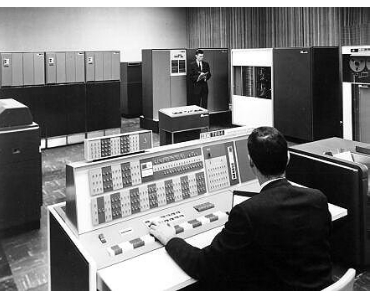
\includegraphics[width=.8\linewidth]{IBM7094.jpg}
  \end{sidecaption}
\end{figure}

En parallèle du perfectionnement des machines et de leur puissance de calcul apparaissent des langages de programmation qui vont faciliter la construction et la diffusion des méthodes de simulation. Nous n'envisageons pas d'en faire un historique complet, mais nous en donnons un aperçu dans l'encadré \enquote{Les premiers langages de programmation}.

\begin{framewithtitle}[Les premiers langages de programmation]{ Les premiers langages de programmation }

La période 1955 - 1965 est une période où la simulation est reconnue comme une méthode de résolution d'un certain nombre de problèmes difficilement tractables mathématiquement.\autocite{Nance1993, Ackoff1961} Des programmes de développement visant à mettre en place des modèles de représentation, de description nécessaire et facilitant la construction de simulations se multiplient. Deux classes de langage informatiques vont voir le jour durant cette période, et vont continuer à se développer et à s'influencer chacune de leur coté jusqu'à encore aujourd'hui. D'une part, les langages de plus haut niveau qui apparaissent ont pour vocation de se positionner comme une alternative plus expressive que l'assembleur. Dans cette optique le premier compilateur FORTRAN apparaît en 1957,  Algol en 1958, Cobol en 1959, et Lisp 1958. Ces langages et leur successeurs sont d'usage assez générique, et permettent de décrire correctement tout types de programmes. Toutefois à l'époque de leur apparition ils sont d'accès relativement difficiles pour une personne non initiée, ce qui nous amène au développements sur la même période d'une deuxième catégorie de langage, plus spécialisée dans la construction spécifique de modèle de simulation. \autocite[239]{Naylor1966}

A la même époque, des langages spécialisés dans l'expression des simulations apparaissent, et pour la plupart s'appuient et évoluent en parallèle des développements des langages classiques sur lesquels ils s'appuient. Ces SPL ( \foreignquote{english}{Simulation Programming Langages}) comme Simula en 1962, ou bien Dynamo en 1958 ont ceci d'intéressant qu'ils ont très largement accompagné les formidables avancées conceptuelles de cette époque et cela au travers des différentes disciplines. Ainsi la première période 1955-1960 est marquée par la mise au point de GSP (\foreignquote{english}{General Simulation Program}) par Owen et Tocher \autocite{Tocher1960}. Celui-ci est considéré comme le tout premier langage mis au point pour faciliter la description de simulation sur ordinateur. Un effort que Tocher va accompagner d'une publication phare en 1963 dans le livre \foreignquote{english}{Art of Simulation} \autocite{Tocher1963} . Vient ensuite une autre génération de langage en 1960-1965 comme GPSS (\foreignquote{english}{General Purpose System Simulator}), Simscript (développé sous l'impulsion de la RAND corporation), et la première version du langage SIMULA, qui donnera naissance à la fin des années 1960 à Simula-67, un langage qui aura un impact dépassant largement la classe des SPL, et inspirera les créateurs des futurs langages objets comme Alan Kay, auteur plus connu comme le créateur du premier langage objet SmallTalk. 

%% FIXME ORTHOGRAPHE DEUX PARAGRAPHE CI DESSOUS
On trouve plus d'information sur cette période spécifique abordé sous l'angle de l'ingénierie logicielle dans les publications de \textcites{Nance2013,Nance1993, Araten1992, Nance2002} et en consultant les \href{http://informs-sim.org/}{@archives} de la WSC (Winter Simulation Conference). Cette dernière, si elle n'est pas la première à aborder cette thématique (le \textit{System Simulation Symposium} en 1957 selon Nance), est la première à vouloir péréniser le débat à un niveau national \autocite{Nance2002}. Fondé en 1967 \autocite{Crain1992, Araten1992} celle-ci jouit aujourd'hui d'une très large visibilité au niveau international, notamment car elle abrite les publications de pionniers et de membres importants pour la discipline simulation. On pourra citer par exemple Sargent et Balci, des pionniers dans la construction de la discipline de la Validation \& Verification, qui participe et publie régulièrement pour cette conférence. 

Dernièrement les \textit{procedings} héberge le récit sur plusieurs années d'un projet \autocite{Nance2013} réunissant les acteurs important dans l'histoire de la simulation autour d'une fondation oeuvrant pour la récolte de témoignages vidéo, audio et la préservation, mise à disposition de tous des documents initiaux fondateurs, le \href{http://d.lib.ncsu.edu/computer-simulation/}{@Computer-Simulation-Archive} hébergé par la \textit{North Carolina State University}

\end{framewithtitle}

\Anotecontent{marble_computer_historycdc}{ \textcite[3]{Marble1967} déclare dans son recueil de programme de 1967 avoir écrit des routines pour le CDC 3400, que l'on suppose rapidement traduit en CDC 6400. Une procédure qui semble courante, comme en témoigne \textcite{Goldberg1968} pour le package \textit{SPURT} dédié à la simulation créé et utilisé (apparemment même par des géographes) au \textit{Vogelback Computing Center} alors sous la direction de Mittman. En 2010 Marble écrit \foreignquote{english}{Northwestern, when I arrived, was just opening its new Vogelback Computing Center and had acquired high end computing technology in the form of a Control Data Corporation (CDC) 6400. Aside from the “super”computer, the most significant component of Northwestern's computing infrastructure, in my eyes, was clearly Vogelback's Director of Computing, Dr. Benjamin Mittman. Ben was the originator of computer chess as a competitive programming activity, and he put together a generally excellent support staff at Vogelback. He was immensely helpful on a personal level to those of us who were working on the CDC mainframe. Ben also made sure that a number of useful software packages (e.g., the BMD statistical analysis package, linear programming software for solution of the transportation problem, etc.) were made freely available to all Vogelback users.} \autocite{Marble2010} Anecdote amusante sur le personnage cité par Marble, Benjamin Mittman est aussi un acteur important dans le développement et la structuration de la communauté créant des programmes d'échecs sur ordinateur, et accueille au \textit{Vogelback Computing Center} les étudiants David J. Slate, Larry R. Atkin, et Keith Gorlen ayant donné naissance au programme pionnier \textit{CHESS} \autocite{Mittman1971} s'executant sur le tout récent \href{http://computerchess.tumblr.com/post/56345790213/playing-chess-at-vogelback-computing-center}{@CDC6400}, vainqueur plusieurs années d'affilé dans les premières compétitions d'échec organisés à l'époque par l'ACM \href{https://chessprogramming.wikispaces.com/ACM+North+American+Computer+Chess+Championship}{@ACM}}

\Anotecontent{ibm604650}{Voir \href{http://www.aag.org/cs/garrison}{@Garrison} et la page \href{https://www.washington.edu/uwit/history/}{@historique} du service IT (information technology) de l'université de Washington}

D'un point de vue technique \textcite{Haggett1969} cite comme véritable point de départ dans la discipline la  démocratisation de l'accès à la ressource informatique après 1961, avec la diffusion d'une deuxième génération d'ordinateurs dans les grands centres de calculs, en partant notamment de la série IBM 7094, le \textit{Vogelback Computing Center} ouvert en 1965 à Northwestern avec un CDC 3400 apparemment très vite completé avec la sortie du CDC 6400 sur lequels vont travailler des pionniers comme Marble \Anote{marble_computer_historycdc}. Des ordinateurs que l'on imagine beaucoup plus accessibles et performants que la précédente série IBM 604 et 650 à \textit{vacuum tube} utilisé au début des années 1960 à l'université de Washington\Anote{ibm604650}, des précurseurs qui seront rapidement remplacés, par exemple par l'IBM 1620 enfin utilisable avec le langage Fortran I \autocite[66]{Berry2005}. 

\Anotecontent{ordinateur_actuel}{En comparaison, les ordinateurs actuels contiennent au minimum 4Go de mémoire, soit 4 194 300 KB.}

En Nouvelle-Zélande, Golledge nous indique que l'installation sur le territoire de la firme IBM semble précéder de peu la formation des pionniers \autocite[94]{Bailly2000}, et au début des années 1960 l'université de Canterbury se porte acquéreur d'un flambant neuf IBM 1620 doté de 32K de mémoire.\Anote{ordinateur_actuel}

\Anotecontent{histoire_suede}{Une récolte de documents publique nationale a été organisé par le \textit{tekniskamuseet} de Suède, les textes sont disponibles à l'adresse internet suivante \href{http://www.tekniskamuseet.se/it-minnen}{@tekniskamuseet}}

En Suède \Anote{histoire_suede}, trois ordinateurs sont construits dans le courant des années 1950-60 : SARA par la société Saab à Linköping, DASK à l'institut scientifique de Copenhague, et SMIL à l'université de Lund \autocite{Persson2007}. Carl Erik Frödberg, un ami d'enfance de Hägerstrand, fait partie avec Eric Stemme des consultants amenés à échanger sur le sol américain avec les leaders du domaine (Neumman, etc.) afin de démarrer le programme suédois.  SMIL est capable de compiler de l'Algol, et c'est probablement sur celui-là que Hägerstrand assisté de Frödberg a pu exécuter ses premiers programmes. En 1969, un Univac 1108 est acheté pour faire suite à SMIL \autocite[33-34]{Lindgren2008}.

En France, en 1955 il y a exactement six ordinateurs \autocite[3]{Armatte2008}, mais c'est seulement en 1970 que l'université Paris 1, centre de référence pour les géographes pionniers quantitativistes, se dote d'un ordinateur Philips et d'un terminal en contact avec le calculateur d'Orsay.

Toutefois, on ne peut parler d'une véritable démocratisation de l'outil informatique chez les chercheurs qu'avec l'apparition dans les années 1970 aux États-Unis des premiers postes informatiques individuels, et il faudra encore attendre le milieu des années 1980 pour que cette technologie se diffuse véritablement et touche le grand public.

A cette période la mise en oeuvre de modèles de simulation est fortement limitée par des problématiques humaines et techniques \autocites{Haggett1969}[387]{Marble1972}, dont on peut constater dans les ouvrages inter-disciplinaires vus dans la section précédente, qu'elle ne touche pas en réalité que la géographie \autocite{Guetzkow1972}.

C'est toutefois dans cette période où les compétences informatiques nécessaires à la programmation se font encore très rares, les langages de programmation multiples et peu stables, le matériel coûteux et peu disponible (nécessitant des opérateurs de saisie, temps d'utilisation partagé entre différentes disciplines, accessible seulement localement), que des packages de programmes sont peu à peu publiés et mis à disposition des chercheurs via les réseaux universitaires \autocite{Haggett1969}. 

Au niveau de ces réseaux de diffusion de programmes, selon \textcite[20-21]{Greer1972} deux sont à noter : \textit{the State Geological Survey of University of Kansas (Computer Contributions)}  et \textit{ the Department of Geography of the University of Nottingham U.K. (Computer Applications in the Natural and Social Sciences) }. Au niveau des progiciels, \textcite[20-21]{Greer1972} identifie en 1972 trois pôles universitaires importants : Iowa \autocite{Wittick1968}, Northwestern \autocite{Marble1967}, Michigan \autocite{Tobler1970c}\footnote{Ces progammes sont malheureusement impossibles à trouver, et les publications ne sont disponibles que sous la forme d'archives numérisées non exploitables (\textit{Google Books}), ou sous format papier dans les universités correspondantes. Un travail reste à faire pour sauvegarder et mettre ce bien commun à disposition de tous les géographes.}. En effet, des pionniers comme Marble ou Tobler mettent à disposition dans le courant des années 1960 différentes routines informatiques en libre accès, \textcite[3]{Marble1967} parle de 150 routines développées jusqu'à 1967, et cela seulement à Northwestern dans le département de géographie. Le premier \textit{Statistical package for Social Science} pour les sciences sociales (ou \href{http://www.spss.com.hk/corpinfo/history.htm}{@SPSS}) date quant à lui de 1968 \autocite{Barnes2011}, alors que sort à la même date l'ouvrage \foreignquote{english}{best-of} de \textcite{Berry1968} \foreignquote{english}{Spatial Analysis: a Reader in Statistical Geography}, qui offre une vision d'ensemble des derniers développements statistiques et mathématiques.

\Anotecontent{programmes}{Particulièrement difficiles à trouver en dehors des Etats-Unis, voici un exemple des rapports disponibles dans les \href{http://findingaids.library.northwestern.edu/catalog/inu-ead-nua-archon-989}{@archives} de la \textit{Northwestern University Library} contenants les précieux programmes et les rapports d'avancements de ces ingénieurs géographes : a) \textit{Duane F. Marble and Sophia R. Bowlby, Computer Programs for the Operational Analysis of Hagerstrand Type Spatial Diffusion Models, Research Report No. 27, February, 1968} ; b) \textit{Duane F. Marble, Some Computer Programs for Geographic Research, Special Publication No. 1, August, 1967 } c) \textit{ Forrest R. Pitts, Hager III and Hager IV: Two Monte Carlo Computer Programs for the Study of Spatial Diffusion Problems, Research Report No. 2, October, 1965}}

En faisant régulièrement état de leur avancements dans divers rapports ou publications\Anote{programmes}, les pionniers Marble, Morrill, Pits et Bowlby \autocite{Pitts1963} qui se placent dans la continuité des premiers travaux relatifs aux processus de diffusion d'Hägerstrand \autocite{Hagerstrand1953, Hagerstrand1967a} donnent ainsi à voir les efforts et les difficultés auxquelles la petite équipe doit faire face pour améliorer les programmes, ou les adapter à des problématiques différentes.

Sur un tout autre front, celui du développement des \textit{large scale models} \autocites[8]{Batty1976}, les universitaires géographes sont plus souvent cités comme spectateurs qu'acteurs \autocite[9]{Batty1994}, cela même si quelques universitaires arrivent à décrocher des contrats importants \autocite{Barnes2006a} pour des études plus pratiques, comme \textcite{Garrison1959}, nottamment du fait que les objectifs poursuivis sont relativement différents, la planification et la prédiction prenant plus souvent le pas sur la curiosité et l'explication scientifique. Toutefois, et si on en croit \textcite{Haggett1969} la communauté universitaire semble attendre beaucoup des retombées de ces grands programmes, qui disposent de moyens humains et économiques importants pour développer des programmes et collecter des données.

Si le requiem de \textcite{Lee1973} a bien eu un effet non négligeable sur la construction et la publication de tels modèles du coté des planificateurs \footnote{Seulement trois modèles seront publiés dans le même journal à la suite de cet article ...}, force est de constater que la construction de modèles de simulation pour la théorie urbaine ne disparaît pas dans cette période \autocite[11-12]{Batty1994}, et s'appuie au contraire sur l'apprentissage de ses échecs pour se réinventer dans les années qui suivent. A ce titre, \textcite{Harris1994} soulève dans une relecture très critique de l'article de Lee, l'ignorance ou la méconnaissance de l'auteur vis-à-vis des débats qui agitent déjà depuis plusieurs années la simulation de modèles urbains \autocites{Batty1971, Wilson1970, Orcutt1957, Harris1968}. Ce faisant, Harris accuse Lee d'enfoncer des portes ouvertes et de porter des accusations que certains jugeront par la suite prématurées vis-à-vis du préjudice subi, touchant à cœur une discipline d'à peine une décennie et encore en phase d'apprentissage. \autocite[p11]{Batty1994}.

Ce mouvement de modélisation doit faire face à l'expression de ces limitations pour se reconstruire, limitations dont on sait par avance qu'elles ne seront pas seulement levées par la seule amélioration des techniques. Ainsi pour \textcite[11]{Batty1976}, de façon plus importante que tous les autres problèmes, c'est la révélation dans l'observation de cette richesse et de cette complexité d'interactions des facteurs causaux à l’œuvre dans l'évolution et la structuration des phénomènes urbains qui va le plus contribuer à la réévaluation des formes de modélisation. \footnote{Une analyse qu'il reprend dans son article de 2001 \autocite{Batty2001}, axée essentiellement autour de l'évolution de l'articulation des mécanismes internes aux modèles et aux répercussions que cela entraîne dans la construction et la validation des modèles.}

D'une part l'emploi de théories trop simplistes, induit indirectement la nécessité d'un retour à une démarche inductive plus exploratoire \footnote{On notera par exemple le témoignage de \textcite{Boyce1988} lorsqu'il dit à propos des chercheurs engagés dans cette voie \foreignquote{english}{Some, including myself, turned to more empirically oriented research activities, perhaps in the hope of strengthening the foundation of future models}}, jusque là mise de coté. 

D'autre part, une autre voie d'évolution possible pour les modèles vient des travaux existants réalisés dans d'autres disciplines universitaires ou dans le monde industriel. Ainsi différentes équipes de développements sont déjà bien identifiées dans la communauté des économistes comme \textcite{Orcutt1960} et son premier modèle micro \foreignquote{english}{bottom-up} développé à l'\textit{Urban Institute}, les démographes sur les modèles de migrations inspirés des travaux d'Orcutt comme REPSIM, puis POPSIM; sans oublier l'apport de \textcite{Forrester1961} sur l'optimisation industrielle, une des branches opérationnelles d'inspiration la plus directe du projet systémique au début des années 1960 \autocites{Cohen1961}[911]{Shubik1960b}.

% et Hagerstrand ? 
La \enquote{micro-simulation} initiée par Orcutt, qui semble effectivement passer outre l'extinction annoncée par Lee en 1973, rencontre même un certain succès durant toutes les années 1970 comme en témoigne la mise en place de nombreux programmes nationaux au début des années 1980. \autocite{Baroni2007} Une réponse à cette survie peut être avancée dans le positionnement innovant d'Orcutt pour faire face aux résultats décevants des \textit{Large Scale Models} de son époque, opérant pour la plupart à un niveau macro et fournissant des résultats hautement agrégés difficiles à exploiter dans un cadre prédictif, et finalement peu représentatifs de la diversité des systèmes économiques \autocites{Birkin2012, Baroni2007}. Si les critiques de Lee peuvent pour la plupart être mobilisées pour critiquer les modèles issus de la micro-simulation (complexité des modèles, absence d'objectifs clairement posés, volume des données à mobiliser, complexité des calculs, coût de construction, absence de résultats, etc.), il n'en reste pas moins que la proposition d'Orcutt introduit avec une approche plus \textit{bottom-up} une dimension explicative absente jusque là. En répondant à l'observation de Lee sur l'absence d'extraction de connaissances micro quelque soit la complexité injectée dans les modèles macro, Orcutt ouvre d'une certaine façon la voie à des développements théoriques beaucoup plus riches que ne le permettaient à l'époque les seuls modèles macro, faisant ainsi de son modèle un instrument pour \foreignquote{english}{consolidating past, present, and future research efforts of many individuals in varied areas of economics and sociology into one effective and meaningful model; an instrument for combining survey and theoretical results obtained on the micro-level into an all-embracing system useful for prediction, control, experimentation, and analysis on the aggregate level} \autocite[122]{Cohen1961}.

D'un autre coté, cette micro-simulation telle que déjà théorisée par Hägerstrand dans sa version spatiale ou par Orcutt dans sa version économique, va étonnamment et cela pendant plusieurs années rester un courant ayant peu d'impact sur le développement des modèles urbains en économie spatiale \autocite[5]{Sanders2006}, et cela malgré plusieurs appels d'un coté \autocite{Hagerstrand1970} ou de l'autre \autocite[5]{Isard1998}. De façon indépendante et dans un univers somme toute limité par de fortes contraintes techniques et financières, ces travaux vont toutefois dans leurs lentes et multiples convergences donner naissance autant à des modèles universitaires qu'à des programmes nationaux (DYNASIM et CORSIM pour Orcutt aux Etats-Unis, SVERIGE en Suède, etc.). Pour finir cette parenthèse sur la micro-simulation par une petite transgression temporelle, si peu de modèles existent encore dans les années 1990, plusieurs publications récentes font état d'un inversion de la tendance ces vingt dernières années \autocite{Lenormand2013}, avec une augmentation (et une diversification ? ) croissante des modèles, sûrement liée à des capacités de développements informatiques plus importants, tant du point de vue des données, que de la puissance d’exécution qui admet l'importance croissante du parallélisme, idéale pour simuler des entités individuelles. \autocites[5]{Sanders2006}{Lenormand2013}

Cette crise, qui on l'a vu touche avant tout les instituts de planification américains couverts par la RAND, va fournir \textit{post mortem} le terreau nécessaire à la transformation d'une discipline dont le rayonnement dans la communauté scientifique à l'international ne va aller qu'en s'amplifiant après 1970 (voir la carte \ref{fig:S_carte_wegener}).

\begin{figure}[h]
\begin{sidecaption}[fortoc]{La carte des centres de recherches les plus actifs à la fin des années 1980, début des années 1990 selon \textcite{Wegener1994}}[fig:S_carte_wegener]
  \centering
 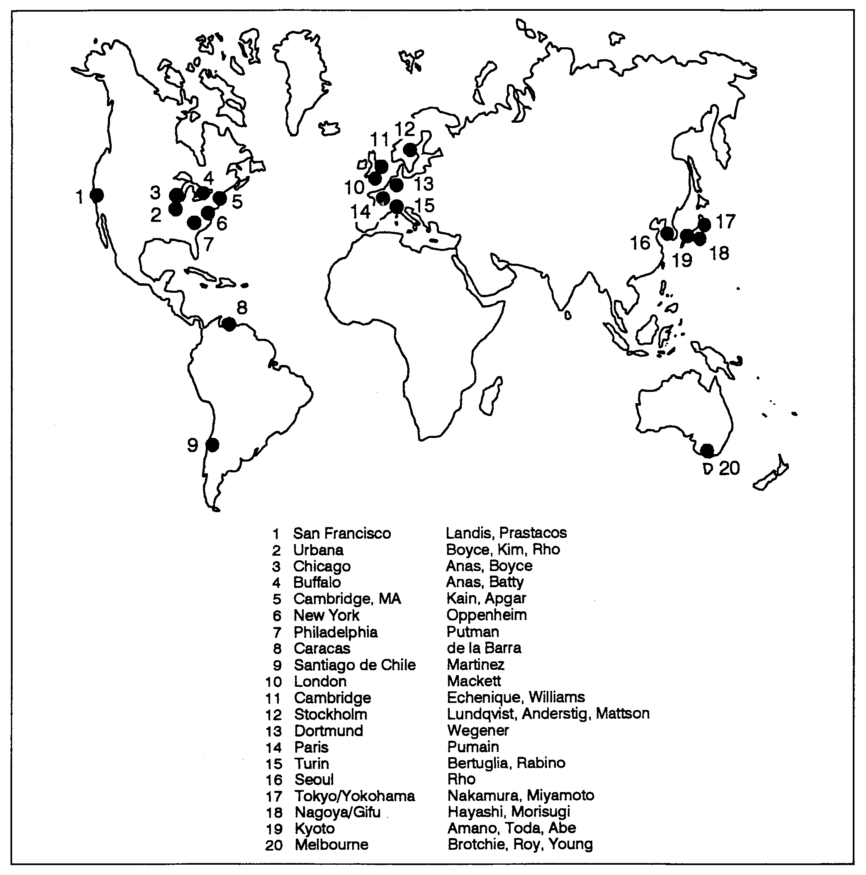
\includegraphics[width=.9\linewidth]{carte_wegener.png}
  \end{sidecaption}
\end{figure}

C'est le cas par exemple au Royaume-Uni où sont récupérés les modèles américains ayant donné de bons résultats, comme celui de Lowry \autocite{Lowry1964}, pour servir de base à de nouveaux travaux mettant en perspective l'influence ou les progrès d'autres courants disciplinaires en contact avec la géographie. 

Le mouvement du professeur Orcutt \autocite{Orcutt1957}, mais aussi celui de Forrester \autocite{Forrester1961, Forrester1969} font dans leur implémentation dynamique alors écho aux travaux initiaux du géographe Hägerstrand, et poussent dans cette période de reconstruction toute une partie des géographes à réintégrer la dimension temporelle à des modèles d'optimisation statique en échec. \autocite[p295]{Batty1976}.

La diffusion et la généralisation du programme systémique permettent aux géographes d'accéder à tous les outils conceptuels et surtout opérationnels \autocite{Forrester1969} nécessaires pour penser, modéliser et simuler les systèmes géographiques au travers de leurs interactions complexes, en intégrant dans leurs analyses cette hétérogénéité d'échelle caractéristique des objets géographiques, comme peut l'être par exemple la région.

Si les universitaires américains semblent rater le coche de cette transformation, en Europe plusieurs écoles viennent à se former, comme la \foreignquote{english}{social physics} de \autocite{Wilson1970} dont l'émergence est considérée comme un moment important dans le renouveau des modèles urbains \autocite{Griffith2010}; mais également d'autres écoles comme celle de Peter Allen, qui s'appuient sur l'évolution des mathématiques et le transfert méticuleux de concepts observés en physique pour construire des modèles à la fois spatiaux et dynamiques capables de simuler de façon plus réaliste les interactions complexes intervenant dans la formation et l'évolution des villes. \autocite[11]{Batty1976, Batty2001} \autocite[27-28]{Pumain2003} \footnote{ Pumain liste au moins trois intérêts qui découlent de cette phase d'acquisition du projet systémique : a) le dépassement de l'opposition idiographique et nomothétique, b) l'histoire et les particularités des entités géographiques vues comme expression originale de trajectoires et de bifurcations, c) le dépassement de la rigidité des trajectoires biographiques historiques par l'emploi des simulations}

\textit{Dans quelles mesures les problématiques levées à la fin de la section précédente ( section \ref{ssec:disciplines_touches}) sont-t-elles encore pertinentes après une telle évolution des pratiques dans la géographie ? }

L'amélioration de la formation des géographes européens, et notamment des géographes français dans les années 1970, permet à ceux-ci d'intégrer plus facilement les évolutions de l'informatique durant les années 1970-1990, leur garantissant ainsi une certaine autonomie de développement qui va donner lieu à plusieurs collaborations fructueuses avec les physiciens \autocite{Pumain1984}; 

Concernant l'accès à la ressource informatique pour construire et explorer les modèles de simulation, même si les conditions se sont améliorées avec la démocratisation de l'ordinateur, celle-ci reste un élément bloquant pour l'exécution et l'exploration des modèles de simulation.

Tout d'abord, il y a ce témoignage\footnote{Ce témoignage est issu d'un échange par mail en 2013} précieux de Duane Marble, un des pionniers modélisateurs américains, qui lorsqu'il est interrogé sur la suite des problématiques de validation des modèles de simulation détaillées dans son article de 1972 \autocite{Marble1972}, conforte d'une certain façon notre point de vue : \foreignquote{english}{As I recall, the situation in the 1980's had not changed very much. Simulation in human geography did not last long. Much of this was the result of a lack of computer capacity. Simply replicating Hagerstrand's diffusion model proved difficult and our attempt to inject a more explicit temporal element just would not work due to the computational load.}

Malgré les apports heuristiques indéniables qui vont avec l'utilisation de l'outil, on retrouve l'expression de difficultés concernant le calibrage des modèles plus complexes chez de nombreux auteurs pionniers modélisateurs \autocites{Batty1976, Pumain1998a}[400]{Sanders1984}, notamment pour ce qui concerne le calibrage des modèles, souvent difficile pour ces modèles dynamiques non linéaires soumis à de tels fluctuations dans leur comportements. Voici comment \autocite{Pumain1998a} résume les difficultés opérationnelles résultats de plusieurs années de travaux menés autour des modèles de simulation dynamiques non-linéaires opérant dans le cadre de la théorie de l'auto-organisation : \enquote{Les difficultés de calibrage, associées à la capacité élevée de bifurcation des modèles, ont été maintes fois décrites, de même que l’impossibilité de valider comme \enquote{meilleur ajustement} une configuration donnée de paramètres.}

Batty est probablement un des premiers géographes à faire ce travail d'état de l'art des techniques de calibrations disponibles et applicables à cette nouvelle classe de modèles urbains. Des méthodes de calibration basées sur des méta-heuristiques de type descente de gradient, sont déjà utilisées par les géographes comme \textcite[159]{Batty1976} pour résoudre des problèmes d'optimisations utilisant les sorties de modèles. Toutefois ces méthodes sont encore trop souvent limitées à des modèles à 1 ou 2 paramètres, et s'avèrent peu robustes face à des problèmes acceptant des minima locaux. 

Une chose est sûre pour ce qui est de la recherche de paramètres, on perçoit très tôt chez certains géographes la nécessité d'optimiser cette étape, rendue improductive et dangereuse du fait de la non-linéarité des modèles \enquote{The trial and error method of searching for best-parameter values by running the model exhaustively through a range of parameter values or combinations thereof represents a somewhat blunt approach to model calibration.}

L'appel à l'utilisation de nouvelles méthodes pour l'exploration des modèles déjà lancés par \textcite{Batty1976}, est par la suite repris de façon implicite par \textcite{Openshaw1996}. Celui-ci publie en 1996 avec un collègue de Leeds un article sur les algorithmes génétiques, la méthode la plus efficace disponible alors pour explorer des espaces de paramètres de façon efficace. La conclusion est explicite :

\foreignquote{english}{The results demonstrate that even GA en ES can provide very good solutions for spatial interaction model calibration, albeit sometimes at the expense of considerable extra compute times. [...] It would also be worth considering the use of other forms of global optimization method; [....] As computer hardware becomes faster, the attraction of simple, relatively assumption-free, and highly robust approaches to global parameter estimation can only grow and allow the geographical model builder to worry less about the problems of parameter estimation and focus more on the task of model design.}\autocite{Openshaw1996}

La course à la puissance informatique nécessaire pour explorer et calibrer les modèles ne fait en réalité que commencer. Les méthodes sont encore en cours de développement, et leur usage s'avère extrêmement coûteux sur le plan informatique.

Se pose alors la question suivante, l'incapacité à calibrer un modèle de simulation n'est-elle pas un problème qui limite de facto l'évolution en crédibilité de l'outil simulation ? 

Concernant ce problème plus large de la validation, dont le calibrage n'est qu'une facette, le changement de paradigme explicatif et l'ouverture sur la complexité a soulevé un débat qui dépasse en réalité la seule problématique technique. Il ne suffit plus de garantir un résultat pour que le modèle soit considéré comme valide, sa structure causale est elle aussi considérée comme le résultat d'un processus social, et dont la contenance doit normalement être validée terme à terme avec le domaine empirique; or c'est celle-là même qu'on ne peut observer dans le cadre d'un système complexe. (cf \textit{observational dilemna} de \textcite[296]{Batty1976} :

\foreignquote{english}{Perhaps the major problem concerns the ability to observe or monitor the urban system. Unlike the physical sciences in which the effect of critical variables on the system of interest can be isolated in the laboratory, such a search for cause and effect is practically impossible in social systems. Thus, there are many instances when it is difficult, if not impossible, to disentangle one cause from another in the changing behaviour of such systems. This is a fundamental limitation which is referred to here as the observational dilemma.}

La dernière phrase d'Openshaw prend alors tout son sens, et en nous rappelant que la construction de modèle est un processus incrémental, il fait indirectement écho à l'évaluation elle aussi incrémentale d'une structure causale où chaque mécanisme lorsqu'il est ajouté/enlevé, remet en cause l'exploration précédente. Dès lors, la systématisation de cette calibration devient \textbf{le seul moyen de garantir une construction} qui serait faite en tout connaissance de cause, en mesurant, et donc en discutant l'apport de chacune des hypothèses durant le processus de calibration.

La dépendance à la ressource informatique se renforce en réalité encore un peu plus avec la nécessité d'explorer les modèles, non plus lorsqu'ils sont terminés, mais dès que la première brique est posée. 

%%FIXME : A MODIFIER POUR COLLER AVEC LE PARAGRAPHE PRÉCÉDENT %%
%Paradoxalement il donne aussi à voir les limites des approches proposées pour létude de l'homme dans son environnement, et offre ainsi le matériel idéal pour appuyer la formulation critique des géographes radicaux marxistes, un mouvement qui s'amplifie dès le début des années 1970 en parallèle avec la conjoncture politique nationale et mondiale. \autocite{Golledge2006}


%Ainsi les progrès fulgurants de l'informatique, l'apparition de nouveaux langages exclusivement orientés pour la simulation comme Dynamo, la prise de conscience tout au long des années 1960-70 des défauts de cette première génération de modèles, et les changements d'objectifs de la discipline \autocite[12]{Batty1994} \autocite{Boyce1988} autorisent (voire recommandent) la formation de nouveaux modèles. Ceux-ci sont conçus comme plus parcimonieux, autorisant les démonstrations plus abstraites \autocite{Forrester1969}, plus orientées vers la compréhension des mécanismes à l’œuvre que sur la prédiction (un retour sur les modèles théoriques est opéré), intégrant plus facilement l'hétérogénéité dans la nature des dynamiques (rétro-action, non linéarité) des processus \autocite{Forrester1969, Wilson1970, Allen1978}, et ouvert à l'intégration d'autres dimensions explicatives à l'oeuvre dans la formation des processus, comme ceux déjà explorés l'individu et le temps \autocite{Hagerstrand1967a,Orcutt1957,Forrester1961}. En lisant les articles de Pred, d'Olsson \autocite{Olsson1969,Olsson1970}, de Curry, on percoit chez les nouveaux économistes spatiaux cette volonté de changement, avec la reintroduction de la stochasticité et des modèles probabilistes, l'intégration du temps dans les modèles, mais aussi les causalités multiples.

% PLUSIEURS points développement méthodologiques accompagnant renouvellement théoriques accompagnant nouvelle géographie : Hagerstrand , Orcutt -> causalité + individualisme méthodologique,  Forrester -> complexité
% Hagerstrand premiere utilisation montecarlo en science sociale, vient a Washington et rencontre Morril... qui pour Benko Stromayer marque troisieme theme dominant le bouleversement quantitatif) Gould2004

% simulation permet de développer cette causalité ...
% Systeme dynamique, non linéarité, permet avancée fondamentale dans les questionnements, révélateur aussi de l'apport des techniques / méthodologies...
% Basculement vers explicatif !


\section{La validation des modèles de simulation}
\label{sec:constante_problematique}

Les termes \enquote{Validation \& Verification} tels que définis par les institutions de normalisation sont conçus comme générique et valable pour des disciplines autres que l'ingénierie logicielle (section \ref{ssec:def_generique_validation}). Dans ce sous ensemble de pratiques, la simulation dispose de sa propre branche historique, dans laquelle des spécialistes raffinent et organisent depuis les années 60 ces notions en mettant en oeuvre des typologies d'outils et des méthodologies de conception et d'évaluation standardisées. \autocite{Nance2002} Si aujourd'hui ces définitions ont évolués et sont parfois reprises pour encadrer des travaux en sciences humaines et sociales, il faut savoir que dans les années 1960-70 celle ci était en l'état peu compatible avec les mutations en cours dans la modélisation en géographie. 

Dans l'histoire de la géographie américaine, le début des années 1970 est marqué comme une période d'émergence de nouveaux courants de géographie. (section \ref{ssec:transition_annee70}) Si il n'est pas question ici de relater en détail cette construction d'une géographie radicale, humaniste ou comportementale, on retiendra seulement que ces courants se forment principalement à la convergence de problématiques politiques (crises économique nationales et internationales, guerres), de revendications théoriques (rejet des méthodes quantitatives et du \enquote{fétichisme spatial} \footnote{\foreignquote{english}{Any approach that treats space as sufficiently autonomous to social processes that ‘no change in the social process or spatial relations could alter the fundamental structure of space’} \autocite[712]{Gregory2009}} ) et/ou méthodologique (retour de l’herméneutique). 

Les acteurs prônant une démarche scientifique teintés de néo-positivisme largement inspiré des sciences physiques sont alors la cible idéale de ces nouveaux acteurs, et vont alors subir un large front de critique. 

Gregory, dont on mobilise le point de vue pour critiquer la vision néo-positiviste/positiviste en géographie, utilise ce dernier argument de façon conjointe avec la pensée d'Habermas pour charger les dérives entraînées par les méthodes quantitatives, et proposer un autre style de pensée axé sur la réconciliation d'un point de vue structuraliste, phénoménologique et critique pour entre autre éviter l'écueil du \enquote{fétichisme spatial}. A la lecture d'ouvrage comme ceux de Gregory, dont la démarche de dépassement n'est pas sans levée des critiques pertinentes, il nous semble a posteriori que sa vision du mouvement quantitatif est en partie biaisé, d'une part parce que la réalité des pratiques peut tout à fait s'éloigner des discours tenus par quelques leaders d'opinion, tel qu'Harvey ou Bunge, et d'autres part parce que les critiques externes au mouvement, comme Gregory font mine d'ignorer une partie des transformations qui opère depuis le début des années 1970 en interne dans les pratiques visés. 

Ainsi, afin de montrer que la discipline géographique n'a pas attendue l'émergence de tels discours parfois extrémistes, nous avons aperçu dans la section \ref{ssec:crise_mutation} que les modèles de simulation économiques spatialisés, ont adoptés au vu de leur maigre résultats une démarche plus explicative permises entre autre par l'évolution des moyens de simulations, et que cette confrontation avec la problématique de validation a été formulé comme centrale par les modélisateurs pionniers et cela de façon explicite dans des ouvrages collectifs abordant cette question \autocite{Marble1972}. Si sur le fond il n'y a rien de critiquable à vouloir développer un autre style de pensée en opposition les excès de certains usages des méthodes quantitatives, sur la forme il en résultent chez certains géographes l'émergence d'un amalgame malheureux qui associe un peu trop rapidement méthode quantitative positiviste, et modèle d'inspiration économique néo-libéraliste \autocite[61-64]{Paterson1984}. Une dualité opposant géographe (et géographie) qualitativiste/quantitativiste encore brandi aujourd'hui comme un processus supposé constructif alors qu'il n'en est rien \autocite{Sheppard2001}.

La section \ref{sssec:realite_neopositiviste} propose de déconstruire avec les arguments disponibles ce point de vue qui voudrait l'application pratique de la méthodologie néo-positiviste comme un support crédible à l'explication dans la construction de modèles en géographie. Une fois cette proposition écartée, la question du devenir des pratiques de \foreignquote{english}{model-building} mobilisé par la géographie quantitative doit être vue sous un autre angle, qui dépasse la seule critique des méthodes de la géographie radicale, celui de la reification du paradigme systémique comme expression formelle adapté à l'analyse complexe des objets géographiques \ref{sssec:progressive_systemique}.

\hl{ A finir intro section}

%Au coeur de la théorie des \enquote{système ouverts} les concepts d'équifinalité, de hierarchisation de statistique sont dans leur opérationalisation \ref{subsec:operationaliser_concept} autant d'incitation à utiliser les récents progrès de l'informatique des années 1950-60 pour explorer un univers, non pas tant complexe dans sa description (comme en témoigne Simon, des problèmes complexes peuvent très bien être dérivé de règle simple) mais dans la multiplicité d'approche (trajectoire, échelles, interactions) qu'elles permettent.

Outre le fait que cette ouverture s'accompagne d'innovation méthodologiques permettant l'opérationalisation des concepts, s'ouvre en parallèle avec la chute du néo-positivisme de nouveaux débats autour de l'explication \autocite{Hedstrom2010} à la fois chez les praticiens (les \enquote{mécanismes générateurs} de Boudon, les \foreignquote{english}{causal-mechanisms} plus récents des biologistes, les \foreignquote{english}{generative mechanisms} d'Epstein) mais également chez les philosophes des sciences en biologie (Salmon, Machamer, etc.) où les thèses de Popper-Hempel, bien que souvent cités, sont en réalité rarement appliqués ou même appliquables dans les faits. \autocite{Bechet2013} 

Un retour sur la démarche de construction des modèles en géographie s'avère nécessaire pour comprendre les éléments qui nous ont échappés dans la continuité de cette problématique qu'est la validation des modèles. En s'appuyant sur les témoignage de \autocite{Batty2001, Pumain2003} on parvient très bien à décrire ce basculement opéré à la charnière des années 1970, alors même que les géographes accède peu à peu aux concepts opérant dans le paradigme systémique \autocite{Harvey1969}, et que l'insuffisance des démarches de construction de modèles devient prégnante.

L'enjeu ici est d'autant plus important qu'il se double d'une réalité opérationelle, faisant des problématiques de sous-détermination (Quine) ou d'équifinalité (Bertalanffy) des concepts tout à fait tangibles, dont la manipulaton débordent du cercle des philosophes des sciences pour venir parasiter les débats des modélisateurs en SHS, dont la qualité des explications avancées doit s'adapter à cet horizon infranchissable, et se réinventer dans des discours, des méthodologies plus spécifiques.

\subsection{Les définitions de la validation}
\label{ssec:def_generique_validation}

Les termes \foreignquote{english}{Validation \& Verification} ou \textit{V\&V} proviennent à l'origine de l'ingénierie des systèmes, et peuvent être rattachés au concept de \enquote{qualité} tel qu'il est défini par la famille de règles ISO établies par l'organisation mondiale de normalisation. 

Décomposable en plusieurs branches cette discipline à part possède une branche dédiée à l'expertise logicielle. De ce fait, il n'existe pas réellement de définition ni de théories ou méthodologies officiellement acceptables, l'acceptation des termes pouvant varier fortement selon les branches d'application. 

On trouve toutefois quelques références dans des livres dédiés à la terminologie standard pour la \enquote{gestion de projet} dans un large panel de disciplines, telle que le PMBOK (\textit{A guide to the project Management Body of Knowledge}) \autocite{PMBOK2013}. Résultats d'un travail certifié par des associations ou des organismes étatiques tels que IEEE et ANSI, ce dernier propose une définition générale de ces termes pour l'ingénierie logicielle : 

\foreignquote{english}{Verification and validation (V\&V) processes are used to determine whether the development products of a given activity conform to the requirements of that activity and whether the product satisfies its intended use and user needs.}

et revient ensuite plus spécifiquement sur les termes : 

\begin{itemize}
\item \textbf{Validation} \foreignquote{english}{The assurance that a product, service, or system meets the needs of the customer and other identified stakeholders. It often involves acceptance and suitability with external customers. Contrast with verification.}
\item \textbf{Verification} \foreignquote{english}{The evaluation of whether or not a product, service, or system complies with a regulation, requirement, specification, or imposed condition. It is often an internal process. Contrast with validation.}
\end{itemize}

Les termes tels qu'ils sont définis sont finalement bien trop généraux pour envisager de les appliquer tels quels dans notre domaine de compétence. Dérivé de la branche de l'\textit{Operational Research (OR)}, les auteurs de la communauté restreinte des \textit{systems analysis or modelling and Simulation (M\&S) } engagent dès les années 1960-70 des efforts pour standardiser ces définitions pour la simulation.

\Anotecontent{first_time_validation}{La citation de Churchman par \textcite{Naylor1966} est tiré de \autocite[165]{Nance2002} : \foreignquote{english}{\foreignquote{english}{X simulates Y} is true if, and only if, (a) X and Y are formal systems, (b) Y is taken to be the real system, (c) X is taken to be an approximation to the real system and (d) the rules of validity in X are non-error-free.} \autocite{Nance2002} }

Parmi les différents auteurs participant de ce mouvement ( Naylor, Finger, Oren, Hermann, Zeigler, Nance, Banks, Gass, Balci, Sargent, etc.), \textcite{Naylor1966} est considéré avec West Churchman (1963) comme un des tout premier à avoir attiré et cristalisé \Anote{first_time_validation} dans de multiples publications l'attention sur cette problématique importante de la V\&V.

Cet économiste formé à l'informatique dans la branche des \foreignquote{english}{management sciences} \autocite{Stricklin1985} est un des premiers en 1967 \autocite{Naylor1967} à publier dans un article nommé \foreignquote{english}{Verification of Computer simulation models} une méthode abordant spécifiquement la question de la crédibilité des connaissances qui peuvent être apportées par un modèle de simulation. Une méthode qu'il va mettre spontanément en tension avec les débats qui agitent la communauté des philosophes à cette même période.

Malgré ces efforts et sa volonté de porter le débat loin dans la communauté inter-disciplinaire (voir les premiers ouvrage collectifs sur l'usage de la simulation dans les \enquote{behavior science} \autocite{Dutton1971, Guetzkow1972} \hl{A verifier}), la démarcation entre les deux termes est encore peu claire \autocites[165]{Nance2002}[3]{Balci1986}. \footnote{\foreignquote{english}{Thomas Naylor, a coauthor of the book cited above, deserves credit for drawing major attention to the validation issue in the 1960s: Is the model actually representing the truthful behavior of the referent system? His work, above and in later publications (Naylor 1971, Naylor and Finger 1967), exerted a major influence in framing validation within different philosophical perspectives. Numerous techniques that can be used were identified or developed. While the issues of both verification and validation were of concern from the early days of simulation, often no clear distinction was made between the two terms.} \autocite[165]{Nance2002}}

\Anotecontent{balci_standard}{\foreignquote{english}{A uniform, standard terminology is yet nonexistent. A recent literature review \autocite{Balci1984} indicated the usage of 16 terms [...] Except some early papers which appearead between 1966 and 1972, model verification and model validation have been most of the time consistently defined reflecting the following differentiation : \textbf{model verification} refers to building the model right; and \textbf{model validation} refers to building the right model. \autocite{Balci1986}}}

Il faudra attendre le début des années 1980 pour qu'un standard émerge, grâce à des financements étatiques \autocite{Balci1986}, mais également du fait des efforts fournis par des auteurs comme Sargent et Balci \autocite{Nance2002}, qui collectent et organisent dans une typologie cohérente l'existant statistique et méthodologique, une activité qu'ils poursuivent encore aujourd'hui \autocite{Balci1998}.\Anote{balci_standard}

Pour \autocite[22]{Oberkampf2010} \foreignquote{english}{A Key milestone in the early work by the OR community was the publication of the first definitions of V\&V by the Society of Computer Simulation (SCS) in 1979 \autocite{Schlesinger1979}}, un des instituts avec la U.S GAO (U.S General Accounting Office) à fournir des spécifications en 1979 \autocite{Balci1986} 

\begin{itemize}
\item \textbf{Model Verification} \foreignquote{english}{substantiation that a computerized model represents a conceptual model within specified limit of accuracy.}
\item \textbf{Model Validation} \foreignquote{english}{substantiation that a computerized model within its domain of applicability possesses a satisfactory range of accuracy consistent with the intended application of the model.}
\end{itemize}

\begin{figure}[h]
\begin{sidecaption}[fortoc]{Un des tout premiers schémas issus de la publication de la SCS \autocite{Oberkampf2010,Schlesinger1979}}[fig:S_VV]
  \centering
 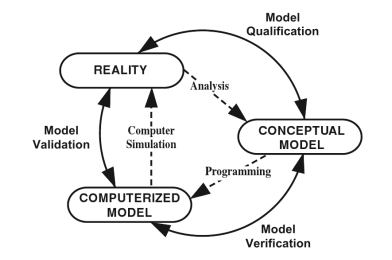
\includegraphics[width=.7\linewidth]{schelinger_schema1979.png}
  \end{sidecaption}
\end{figure}

Même si elles sont plus anciennes et de portée moins générale, ces définitions de la \textit{V\&V} semblent plus pertinentes, car évoquées plus régulièrement par les chercheurs en sciences sociales; les travaux les plus cités étant ceux de \textcite{Kleijnen1995}, ou \textcite{Sargent2010} qui placent leurs travaux dans la continuité de ces définitions. L'avancée de leurs travaux peut être suivie en feuilletant les \textit{Proceedings of the Winter Simulation Conference} où la problématique de la \textit{V\&V} est réévaluée régulièrement au regard des nouvelles connaissances. Ce schéma \ref{fig:S_VV} est devenu un classique repris et régulièrement amendé \autocite{Sargent2010}. Voici la lecture qu'en fournit \autocite{Oberkampf2010} 

\foreignquote{english}{The \textbf{conceptual model} comprises all relevant information, modelling assumptions, and mathematical equations that describe the physical process or process of interest. [...] The SCS defined \textbf{qualification} as \enquote{Determination of adequacy of the conceptual model to provide an acceptable level of agreement for the domain of intended application}. The \textbf{computerized model} is an operational computer program that implements a conceptual model using computer programming. Modern terminology typically refers to the computerized model as the computer model or code.}

Ce schéma a la particularité suivante, il \foreignquote{english}{ [...] emphasizes that \textbf{verification} deals with the relationship between the conceptual model and computerized model and that \textbf{validation} deals with the relationship between the computerized model and reality. These relationships are not always recognized in other definitions of V\&V [...]}

\Anotecontent{Kleijnen_def}{\foreignquote{english}{This paper uses the definitions of V \& V given in the classic simulation textbook by Law and Kelton (1991, p.299): \enquote{Verification\textbf{Verification} is determining that a simulation computer program performs as intended, i.e., debugging the computer program .... \textbf{Validation} is concerned with determining whether the conceptual simulation model (as opposed to the computer program) is an accurate representation of the system under study}. Therefore this paper assumes that verification aims at a \enquote{perfect} computer program, in the sense that the computer code has no programming errors left (it may be made more efficient and more user friendly). Validation, however, can not be assumed to result in a perfect model, since the perfect model would be the real system itself (by definition, any model is a simplification of reality). The model should be \enquote{good enough}, which depends on the goal of the model.}}

\Anotecontent{Sargent_def}{\foreignquote{english}{\textbf{Model verification} is often defined as \enquote{ensuring that the computer program of the computerized model and its implementation are correct} and is the definition adopted here. \textbf{Model validation} is usually defined to mean \enquote{substantiation that a computerized model within its domain of applicability possesses a satisfactory range of accuracy consistent with the intended application of the model} \autocite{Schlesinger1979} and is the definition used here. A model sometimes becomes accredited through model accreditation. Model accreditation determines if a model satisfies specified model accreditation criteria according to a specified process. A related topic is model credibility. Model credibility is concerned with developing in (potential) users the confidence they require in order to use a model and in the information derived from that model. A model should be developed for a specific purpose (or application) and its validity determined with respect to that purpose}}

Autrement dit, \foreignquote{english}{The OR community clearly recognized, as it still does today, that V\&V are tools for assessing the accuracy of the conceptual and computerized models.} Un avis partagé par \autocite{Kleijnen1995} \Anote{Kleijnen_def} et \autocite{Sargent2010} \Anote{Sargent_def} mais également des auteurs de références sur le sujet dans les sciences humaines et sociales \autocite{Amblard2006} \hl{Prend le bout de texte la dessus}.

Seulement, cette forme de relâchement sur la correspondance entre réalité et modèle, et ce positionnement plus relativiste de la validation n'a pas toujours été une évidence; les premières définitions de Naylor par exemple, sont toujours usitées, et continuent si on en croit des auteurs comme \textcite{Kleindorfer1998} à semer le trouble dans certaines disciplines.

\Anotecontent{VV_philout}{ \foreignquote{english}{During the last two decades a workable and constructive approach to the concepts, terminology, and methodology of V\&V has been developped, but it was based on pratical realities in business and government, \textbf{not} the issue of obsolute thruth in the philosophy of nature} \autocite{Oberkampf2010} 
\foreignquote{english}{A very old philosophical question is: do humans have accurate knowledge of reality or do they have only flickering images of reality, as Plato stated? In this paper, however, we take the view that managers act as if their knowledge of reality were sufficient. Also see Barlas and Carpenter (1990), Landry and Oral (1993), and Naylor, Balintfy, Burdick and Chu (1966, pp.310-320).} \autocite{Kleijnen1995}
\foreignquote{english}{With the strong interest in verification from the software engineering community, this contrasting but complementary explanation of the term was quite important. The effort to place valida- tion in a cost-risk framework moved the concept from a philosophical explanation in earlier works to a form more useable for simulation practitioners.} \autocite[165-166]{Nance2002}}

Mais en excluant ainsi de son analyse la partie subjective et philosophique de la \enquote{Validation}\Anote{VV_philout} pour se concentrer sur la seule partie opérationnelle, ces méthodologies restent pour le modélisateur une coquille vide décevante, qui demande encore à être incarnée thématiquement. Autrement dit, ces méthodes si elles prennent bien en compte la dimension dynamique et incrémentale nécessaire à la construction d'un modèle de simulation qui tendrait vers une réalité en accord avec la question posée, l'organisation des connaissances nécessaires pour guider ce processus reste à la lecture de ces typologies une opération quelque peu énigmatique pour les modélisateurs géographes. On retombe sur une des critiques soulevées précédemment dans la section \ref{sec:critiques_simulation} sur l'absence constatée dans les publications de méthodologie standard pour la validation qui prendrait en compte les problématiques spécifiques d'une discipline. \footnote{Aujourd'hui des disciplines comme l'écologie proposent des méthodologies plus spécifiques, comme la méthode POM proposé par Grimm sur lequel nous reviendront par la suite \hl{mettre une ref et un appel à la section}}

Une position compréhensible pour ces auteurs en mission de standardisation, alors même que ces termes sont toujours d'usages assez variables. Une des conséquences visibles tient dans ces incompréhensions et ces débats terminologiques sans fin \autocite{David2009} que l'on observe parfois en marge des discussions inter-disciplinaires. Cette gamme d'acceptions différentes tient souvent au transfert hasardeux des terminologies entre l'ingénierie des M\&S, la philosophie des sciences, et la thématique d'un chercheur en sciences sociales qui se retrouve en position intermédiaire de ces deux derniers. Un exercice d'équilibriste périlleux, car comme le fait remarquer \textcite{Kleijnen1995} en citant astucieusement une note de bas de page de \textcite{Barlas1990}, en philosophie il est tout à fait possible de voir la signification des deux termes inversée! \hl{Expliquez mieux que verification pourrait se traduire en philosophie pour certains par representation de la vérité, du “reel”, alors que le fait même de modéliser implique qu’on en soit loin}

Pour conclure sur cette partie, si la communauté M\&S propose aujourd'hui un cadre d'analyse cohérent avec la dynamique attendue chez les géographes pour la construction des modèles, il lui manque toutefois une incarnation géographique qu'il va falloir extraire de nos propres exigences de construction.

\hl{Pour comprendre comment la notion de validation se construit en marge de ces deux discours, il faut revenir sur ce qui fait sens dans l'explication pour les géographes. En repartant des transformations que subit la géographie quantitative dans les années 1970 au contact du paradigme systémique, prise dans une nouvelle réflexion des objets géographiques , dont la percolation chez les géographes s'observe dans la nouveauté le champs lexical, les méthodes, mais également les techniques.}

\subsection{Le tournant explicatif des années 1970} 
\label{ssec:transition_annee70}

\subsubsection{Quelle réalité dans l'application de la démarche explicative néo-positiviste}
\label{sssec:realite_neopositiviste}

La question de la validation des modèles est donc à replacer dans le contexte plus général de la recherche d'explication. Les critiques se concrétisent dans au moins trop points que nous détaillons par la suite : celle objective de l'échec de la philosophie logique néo-positiviste comme projet réaliste pour l'explication, l'inadéquation des démarches méthodologiques de géographes ayant adhéré à ce programme, trop éloigné des pratiques réelles des scientifiques, et enfin l’échec des modèles centrés sur la prédiction qui renvoient à la transformation des pratiques de modélisations. Trois points que nous détaillons ci-dessous.

\paragraph{Un état critique du débat épistémologique néo-positiviste dans les années 1960-70}
\label{p:critique_debat}

Dès 1940 Hempel, un des membres influents dans le cercle de Vienne, s'intéresse de plus près à la problématique de la \enquote{confirmation} dans le cadre du modèle hypothètico-déductif, nommé par la suite H-D confirmatif. Il va alors être le premier à s'interroger \enquote{[...] non pas sur la formulation d'une hypothèse ou d'une loi universelle à partir de cas particulier, mais sur la \textit{confirmation} d'une hypothèse ou d'une loi donnée} \autocite{Lecourt2006}. Cette démarche va connaitre rapidement plusieurs difficultés, avec l’avènement de plusieurs paradoxes bousculant les démonstrations logiques, comme le paradoxe de Goodman, ou celui d'Hempel (Raven Paradox). Certains paradoxes seront résolus dans différentes déclinaisons du modèle H-D, mais d'autres resteront problématiques, amenant peu à peu à l'affaiblissement de l'approche cumulative empiriste. \hl{Paradoxe a détailler concrétement !}

Dans les convergences entre faillibilisme Popperien et positivisme logique, il existe des divergences aussi fortes que ne peuvent être les convergences. Ainsi à méthode H-D quasi-similaire, l'hypothético-déductivisme de Popper impose pourtant un raisonnement inverse pour la formulation des hypothèses. Il ne s'agit plus d'une formulation pour la construction incrémentale de loi ou de théorie, mais d'une formulation dont la fonction est avant tout de déstabiliser une théorie ou une loi existante. Pour Popper la science avance dans une perspective critique, la théorie de la relativité d'Einstein fournissant un parfait exemple de situation où le seul échec d'une expérimentation peut remettre en cause toute un pan de la théorie. Dans le langage de Popper, l'hypothèse devient conjecture, et la vérification est donc empreinte d'un double sens : une corroboration en cas d'une confrontation positive, et une falsification en cas de confrontation négative. Avec cette particularité que lorsque la conjecture est vérifiée, celle ci est d'un apport beaucoup plus faible que dans le cas d'une vérification, du fait des nombreux paradoxes qui accablent le \enquote{problèmes de l'induction}, et que Popper veut écarter définitivement du processus de démarcation entre science et non science.

Popper, rationaliste et plus proche critique des méthodes des positivistes logiques va proposer un modèle H-D en négatif qui remet en cause complètement l'empirisme des positiviste logiques. Celui-ci, de nouveau compatible avec la métaphysique, ne supporte plus une logique de confirmation mais de réfutation comme moyen pour séparer science et non-science.

La méthode H-D de confirmation permet de rejeter ou d'accepter des énoncés observationnels, mais elle ne constitue pas en elle même une méthode \enquote{explicative}. La méthode Déductive Nomologique (D-N) formulé par Hempel et Oppenheim’s  est en 1945 une tentative tout à fait originale pour créer une logique formelle centrée sur l'explication.

\hl{Explication rapide modèle ND}

Des discussions internes et externes de ce programme néo-positiviste s'étalant sur plusieurs dizaines d'années ressortent deux modèles en définitive compatibles, le modèle Hypothético Déductif H-D pour la \enquote{falsification/corroboration} de Popper et Déductif Nomologique (D-N) (connu aussi sous le nom de \foreignquote{english}{covering law}) pour \enquote{l'explication} de Hempel-Oppenheim ou encore Hempel-Popper.

Il ne s'agit pas de rentrer dans les détails des critiques qui ont étés faites à ces deux versions de modèles ici, tant elles ont été nombreuses, et sur ce sujet on pourra se rapporter aux ouvrages de \textcite{Chalmers1987}, \textcite[214-215]{Meyer1979} et du coté des épistémologues géographes au travail de \autocite{Besse2000}. En définitive, et c'est probablement là le principal argument qui rend désuet l'appel encore aujourd'hui à une telle philosophie, les principaux acteurs de cette méthode, comme Hempel, le principal artisan de la méthode N-D abandonne définitivement le modèle vérificanioniste en 1950-51, et le falsificationisme en 1965. Des dates qui illustrent le décalage temporel existant avec les tentatives des théoriciens comme Harvey d'adhérer à une telle démarche en 1969, alors qu'elles sont d'ores et déjà dépassées.

%Parmis les défaut principaux qui paraissent poser problème pour un usage raisonné de cette méthode dans la discipline, a) il est impossible de différencier logiquement une loi d'une simili-loi, comme cela pourrait être le cas en géographie; b) le modèle D-N n'est pas universel ; c) la complétude dans l'explication scientifique est un mythe, et même si elle était possible était universellement possible, n'est pas un gage de scientificité, et inversement; c) la symétrie entre explication et prédiction n'est pas vrai; toute prédiction n'est pas explicative et inversement; c) le modèle est linéaire, une cause entraînant un effet, peu compatible avec la complexité du monde réel; d) le processus de découverte se situe en dehors de l'analyse e) la conclusion est contenu dans les premisses ; f) l'explication est en réalité plus justification, et ne rend pas forcément compte des processus générateur

%\hl{Colle pas avec la suite, soit il manque le développement, soit il faut le déplacer plus haut dessous le modele ND qui reste à détailler }
%Deux choses peuvent nous intéresser particulièrement dans ces critiques. D'une part non seulement ce modèle est loin d'être universel, et ne garantie aucunement l'explication, c'est l'objet du premier paragraphe. D'autre part la remise en cause de la symétrie entre explication et prédiction car toute prédiction n'est en soit pas explicative et inversement, et fera l'objet d'un deuxième paragraphe. 

%Les faiblesses dont il sais déjà qu'elles existent : ignorance de la recherche comme activité, symétrie entre explication et prédiction, absence de découvertes autres que celle contenue dans les prémisses.

\paragraph{Les principaux instigateurs du mouvement en géographie}
\label{p:instigateurs_mouvement}

Si il est clair que le positivisme logique n'est pas au fondement de la révolution quantitative \autocite{Claval2003}, l'impact de ce mouvement sur la géographie dans la décennie 1960-70 existe, ne serait ce que par la portée des théoriciens qui ont bien voulu s'en faire le porte voix, cela de façon implicite comme Bunge, ou plus  explicite comme Harvey. La mesure de cet impact reste par contre difficile, sinon impossible à quantifier.

La première introduction au positivisme logique chez les géographes semble au départ se limiter aux étudiants présents sur les bancs de l'université de Washington (Seattle) et d'Iowa \autocite[554]{Barnes2001a} \autocite[120-121]{Unwin1992}, ce qui concerne aussi les étudiants en déplacements pour leurs études du fait des échanges internationaux réguliers et caractéristiques de la tradition anglo-saxonne.

Un bon point de départ pour observer la diffusion de ces méthodes semble être l'histoire personnelle de Schaefer. Il semblerait que la communauté des géographes soit en accord \autocite[15]{Louail2010} pour désigner l'article de Fred Schaefer \autocite{Schaefer1953} comme le catalyseur des frustrations d'une génération de géographes envers les pratiques alors en cours dans leur discipline, en déclin tant d'un point de vue scientifique qu’institutionnel.

Né à Berlin, Schaefer profite d'une solide formation inter-disciplinaire en Allemagne, qu'il fuit dès lors qu'il est apparenté à un terroriste par les Nazis, du fait de ses appartenances politiques. Après un court exode en Grande-Bretagne, il s'installe aux État-Unis où il participe à la diffusion de la géographie économique Allemande, par des enseignements, mais également par le biais de traduction (Lösch). \autocite{Bunge1979}

A la lecture de son fameux article méthodologique \textit{Exceptionalism in Geography} l'influence du programme des positivistes logiques est évidente. Rien de surprenant à cela, en effet Schaefer meurt en 1953, et c'est son ami proche Gustav Bergmann qui prend en charge la relecture et la publication finale dans les annales de l'AAG. \autocite[32]{Gregory1978}. Philosophe proche du cercle de Vienne et lui aussi exilé, Bergmann va enseigner la philosophie à la faculté d'Iowa dès le débuts des années 1950, tout en restant très proche et très influent auprès des jeunes géographes.\autocite[192]{Buttimer1983} Ainsi, King, Clarke, Golledge, et Johnston, sont tous passés par les bancs des universités néo-zélandaises et américaines et ont ainsi joué un grand rôle dans la diffusion de la géographie quantitative mais aussi du néo-positivisme dans ce pays. King, qui dispense des cours d'analyse spatiale à Canterbury dans les années 60 est passé en 57 à Iowa, et Golledge nous dit avoir suivi les cours de Bergman lors de son séjour dans cette même université \autocite[95-96]{Bailly2000}. \footnote{Pour plus d'information sur la diffusion du néo-positivisme en Nouvellve Zélande, on pourra se référer plus spécifiquement à la thèse de \textcite{Hammond1992}}

L'impact premier de cet article de Schaefer est difficile à évaluer, car celui ci ne devient un référentiel que quelques années plus tard, une fois repris par d'autre théoriciens \autocite[32]{Gregory1978} L'ouvrage en 1962 de William Bunge, premier grand théoricien de cette \enquote{révolution quantitative}, bien que faisant une référence implicite à ce mouvement, joue un rôle important dans la diffusion de ce standard scientifique. Enseignant également à l'université de l'Iowa, celui ci va se positionner sur la même ligne que son collègue et ami Schaefer \autocite{Goodchild2001}, et affirmer dans un article fondateur \autocite{Bunge1962} sa volonté d'une géographie avant tout nomothétique, comme les autres \enquote{sciences}. \autocite{Bunge1979} \autocite{Claval2003} \autocite[429-430]{Gregory2009}. 

Un autre point de vue plus tardif mais cette fois ci explicitement teinté de néo-positivisme est réalisé par Harvey en 1969 \autocite{Harvey1969}. Bien que le travail d'Harvey soit reconnu comme un apport bénéfique à la géographie par de nombreux relecteurs (Amadeo, Gregory, Wolpert), ce travail à la fois très dense et écrit sans réel public cible en tête touche finalement une audience relativement limitée, notamment du coté des étudiants, qui disposent déjà de nombreux autres ouvrages connus comme référence (Gregory 1963, Chorley et Hagget 1965, Abler 1971) \autocite{Johnston2008}. \hl{numéro de page ou citation ici !}

Connu pour son exploitation de la philosophie néo-positiviste, \textit{Explanation in Geography} est le fruit d'un travail d'écriture de longue haleine, conçu avant tout comme une position de recherche, autant de présupposés prémonitoires selon \textcite[47]{Barnes2006b} des critiques à venir. L'écriture de cet ouvrage est donc à remettre dans un contexte spécifique, en 1960 dans l'université provinciale de Bristol, ce qui fait plus de ce livre selon Barnes \autocite[31-36]{Barnes2006b} un manifeste énergique destiné à électriser la discipline, et à motiver la modernisation des institutions d'enseignement britanniques.

L'application d'une étiquette néo-positiviste à la géographie quantitative des années 1960-70 n'est pas si évidente, et une relecture plus critique de cette période permet de relever d'autres motivations, qui mettent tout autant en défaut le discours globalisant des théoriciens comme Harvey, que les discours critiques des géographes radicaux rejetant en bloc toutes les approches quantitatives.

\paragraph{Une étiquette néo-positiviste critiquée et critiquable}
\label{p:etiquette_neopositiviste}

De lecture difficile car très abstrait et mathématique, l'ouvrage d'Harvey constitue une tentative intéressante d'introduction de l'épistémologie des sciences au géographe bien qu'il reste avant tout motivé par la description d'une \enquote{démarche scientifique idéale} plus que d'une lecture rigide de l'orthodoxie prônée par les positivistes logiques. Écrit semble t il dans un certain isolement vis à vis du monde (selon ses propres termes), on comprend mieux pourquoi Harvey choisit dans son ouvrage de défendre une démarche scientifique qui sur la fin des années 1960 est déjà très largement critiquée, voire abandonnée par les autres philosophes des sciences. \autocite[147]{Ouelbani2006}. Mais en prônant cette posture délicate, Harvey s'expose tout autant aux foudres des philosophes, pour qui une attitude plus laxiste pourrait trahir la logique des démonstrations en place, que les foudres des géographes depuis longtemps enclins à la pratique d'autres types de démarches scientifiques.

%\autocite[57]{Harvey1969}

En 1972, l'ouvrage \textit{Explanation in Geography} est très vivement attaqué par une critique longue et argumentée de \textcite{Gale1972} dans le très sérieux journal \textit{Geographical Analysis}. Bien qu'Harvey présente d'autres démarches explicatives dans son ouvrage, et présente une lecture quoique superficielle, mais lucide des critiques énoncées sur la démarche néo-positiviste, il choisit quand même un alignement sur l'explication nomologique-déductive, moyennant le relâchement de certaines contraintes \autocite[39-40]{Paterson1984}. Ce qui en fait selon \textcite{Gale1972} un ouvrage propice aux débats, mais d'un autre usage limité, car cette posture de l'auteur, fluctuant autour de ce logicisme philosophique introduit de nombreux paradoxes dans l'argumentation de l'auteur.

Si on peut tout à fait accepter la volonté d'Harvey d'assouplir dans son argumentaire \footnote{On pensera notamment à l'assouplissement de la notion de loi de couverture universelle pour tout temps et tout espace ... } une démarche analytique de toute façon construite elle même plus comme un idéal à atteindre qu'une réalité dérivée des pratiques des scientifiques \footnote{Cette position n'est en soit pas réellement un problème, Hempel positionnant lui même sa méthode dans ce même idéal \autocite{Besse2000}}, il est toutefois beaucoup plus paradoxal de voir Harvey s'aligner en définitive sur le modèle néo-positiviste, une démarche scientifique analytique et réductionniste \autocite[57-59]{Paterson1984} basée sur le déroulement d'un modèle usant de causalité linéaire pour l'explication, alors que celui ci se dit lui même convaincu de l'éminente complexité des processus dans le temps sous-jacents à l'établissement des régularités spatiales observées et de leur importance dans l'explication.

Ainsi, dans le chapitre sur le modèle d'explication systémique de \textit{Explanation in Geography}, c'est tout à fait conscient de l'absence d'expression opérationnelle de cette méthode qu'il expose tout de même sa foi envers cette nouvelle méthode en cours d'intégration par les géographes \autocite[449,469]{Harvey1969}, en supposant que \foreignquote{english}{Whatever our philosophical view may be, it has been shown that methodologically the concept of system is absolutely vital to the development of a satisfactory explanation} \autocite[479]{Harvey1969}

Autre paradoxe, alors que la seule \enquote{loi} est censée piloter l’expérimentation dans cette démarche nomologique-déductive, Harvey admet toutefois la nécessité pour la géographie \enquote{d'une amorce} empirico-déductive, un élément important de cette révolution quantitative, ne serait ce que parce que la géographie ne possède jusque là, il est vrai, que des lois d'emprunt \autocite[41-42]{Harvey1969}. Alors que les points de vue de Hempel et Popper convergent pour affirmer leur opposition à toute \enquote{logique de la découverte}, cette entaille au protocole avancé par Harvey n'est pas anodine. Dans la démarche de progression scientifique proposée par Hempel-Popper, la seule méthode valide pour faire le tri parmi l'infinité de faits disponible doit se faire par la corroboration ou la réfutation d'une inférence déductive. La formulation de l'hypothèse se fait donc \textit{a priori}, par généralisation accidentelle, ou par intuition scientifique, ce qui rend toute logique de la découverte externe au processus objectif scientifique et renvoie cette problématique à la psychologie. Une vision déjà nettement critiquée par \textcite{Simon1973}, où il attaque largement le point de vue de Popper dans son article \textit{logic of discovery} dont il juge le titre particulièrement hypocrite compte tenu des remarques faites ci dessus. 

De plus, l'explication comme activité, ou processus en vue d'organiser des connaissances communicables n'est pas prise en compte par le point de vue des épistémologues; or Harvey en est bien conscient lorsqu'il réalise son grand écart \autocite[10]{Harvey1969}, les géographes ne s’intéressent pas tant à la problématique de l'explication \textit{per se}, mais plutôt à son utilisation dans un contexte donné, celui du champ scientifique des géographes.

Malgré tout, Harvey propose une démarche de construction des modèles qui reconnaît le rôle a priori des théories sur les données, démarche qu'il oppose à la démarche classique inductive Baconienne. Le \enquote{problème de l'induction} étant ce qu'il est, irrésolu, l'inférence statistique n'est permise que dans un cadre formel orienté vers la déduction, pour la corroboration ou la réfutation d'une conjecture.

\hl{Ici il y a deux raisonnements qui se chevauchent, à clarifier donc }
Or non seulement aujourd'hui alors qu'il y a une différence entre loi phénoménologique et loi mais il est d'ores et déjà admis qu'il est aisé de maintenir une théorie coûte que coûte en biaisant l'expérimentation \footnote{\hl{Voir la critique de Chalmers sur Popper...} }, ce qui rend susceptible toute théorie de mentir tout autant que les observations; mais l'utilisation des méthodes statistiques descriptives, multi-variées comme la régression multiple, les analyses factorielles, les statistiques spatiales dans une démarche empirico-inductive joue évidemment un grand rôle dans la capacité des scientifiques à construire des modèles, des expérimentations permettant de comprendre la complexité des masses de données en dehors de toute dépendance à une loi. %L'organisation hiérarchique ordonné des connaissances pyramidal proné par la \enquote{méthode standard}, défendu sans être réellement explicité par Harvey est un modèle d'organisation désuet depuis qu'il est possible de mettre face à face le modèle ondulatoire et corpusculaire pour décrire la même réalité, un point de vue que l'on retrouve dans la convergence de pensée de Ian Hacking \autocite[348-351]{Hacking1983} et les travaux de Nancy Carthwright  dans \textit{the mappled world} et \textit{How the law of physics lie}.

% modele 

En s'appuyant sur cet état de fait, on peut mobiliser l'argumentaire de \textcite{Wilson1972} pour montrer que l'approche proposée par Harvey est bien loin de ce qui est réalisé en pratique. Celui ci voit bien cette dualité qui existe entre les deux courants majoritaires de modélisation, avec d'un coté cette géographie théorique issue de la branche \foreignquote{english}{Models in Geography} qui manque de données pour tester ses hypothèses, s'avère limitée dans son expression opérationnelle (les modèles micro trop complexes, la validation et la calibration encore difficiles), et met selon lui encore trop l'accent sur l'induction statistique et pas assez sur la démarche hypothético-déductive pour former des modèles \footnote{Modèle est ici synonyme pour lui de théories} ; et à l'inverse la branche instigatrice des \textit{large scale models} qui fait (trop) usage des dernières techniques, dispose de large données, mais s'avère incapable du moindre résultat car mal équipée en termes de théorie, guidée par des objectifs divergents, où la prédiction est souvent le résultat d'un \enquote{camouflage} usant des \foreignquote{english}{Goodness Of Fit} de l'économie \autocite[10]{Batty1994}.

\hl{Hors sujet ici }
Même si les problèmes d'autocorrélation spatiale, associés au \enquote{problème de l'induction} limitent effectivement la portée des généralisations qui peuvent être faites, cela n’empêche absolument pas son utilisation dans le cadre réaliste des pratiques scientifiques, et cela on imagine durant tout le processus de construction des modèles.

%\textcite{Barnes1996} produit une contre-narration intéressante sur des acteurs majeurs dans la formation de la révolution quantitative, comme Isard, Bunge, Warntz, Haggett; et prend ainsi le contre-pied de l'analyse classique plaçant la nouvelle géographie sous la seule influence d'un néo-positivisme. 

Ce constat est appuyé par les travaux de Barnes qui propose une relecture critique de l'histoire de la géographie économique \autocite[122]{Barnes1996} à travers une analyse des textes et des pratiques d'acteurs importants tel que Warntz, Isard, Bunge, ou encore Haggett. C'est à ce titre qu'il affirme \autocite{Barnes2001a} le fait que bien des acteurs de la première vague théorique semblent ne jamais avoir rencontré de positiviste \footnote{Morrill1993 citation à récupérer}. Entre autre anecdote qui renforce encore ce sentiment d'une philosophie en décalage avec les pratiques, le philosophe néo-positiviste Bergman, proche des grands géographes théoriciens, n'est pas un des plus grands adeptes d'une application stricte de la \foreignquote{english}{scientific method} aux sciences sociales \footnote{Dans le recueil de texte biographique \textit{Mémoires de Géographes} \textcite[96]{Bailly2000}, Golledge revient sur les propos de Bergman : \enquote{Bergman soulignait la différence entre ce qu'il appelait alors la science pure et la science sociale. C'était le premier à admettre que l'utilisation des procédés logiques positivistes dans la science sociale pourrait se révéler extrêmement improductive.} } 

\paragraph{Un échec et des critiques qui ne doivent pas masquer la réalité des transformations}
\label{p:echec_critiques}

%La problématique des modèles \enquote{a priori} défendu également par Harvey peut être en partie retrouvé dans les critiques qui sont opposés aux ouvrages et aux projets inspirés par cette démarche néo-positiviste.

Pour \textcite[41]{Gregory1978} le relâchement des contraintes préconisé par Harvey \autocite[47]{Paterson1984} autorise le développement pour la géographie \foreignquote{english}{[...] a \enquote{weaker} paradigm of explanation and theory, altough one \enquote{not entirely unrelated} to the \enquote{scientific} paradigm}, paradigme basé sur \foreignquote{english}{the willingness to regard events \enquote{as if} they are subject to explanation by laws \autocite[174]{Harvey1969}}. 

Une forme d'instrumentalisme \footnote{Selon \textcite{Gregory1978} \foreignquote{english}{instrumentalism regards theories as devices whose utility is at stake; their truth cannot be an issue since no conclusive can be provided for them, and so science is justified in adopting a more pragmatic set of standards in whichs its propositions are evaluated to the success of their predictions and nothing else.}} qui renvoie la modélisation à un seul objectif prédictif, qui appuie selon lui une application néo-libérale \footnote{\foreignquote{english}{Instrumentalism plays an important supporting role in neo-classical economics, and so it is not surprising to discover that is has been carried over into much of modern geography, where its emphasis on \foreignquote{english}{goodness of fit} had had two consequences [...] First, it has allowed an extremely narrow, even superficial, formulation of spatial process to emerge, in which space-time variations are made to conforme to a typology of corresponding forecasting models. This is frequently helpul, of course [...] but the empirical identification of appropriate model structures ought not to become a substitute for the proper specification of the mechanisms involved. [...] Secondly, [...] instrumentalism has promoted a limited, at times almost an opportunist, image of geography as policy science. [...] Olsson (1972) and Lewis and Melville (1977) have shown that the instrumental approach of the social engineer dominates geography and the other regional sciences \textit{in general} \autocite[41]{Gregory1978}}}.

Gregory fait surement ici écho aux résultats médiocres \autocite{Lee1973} d'une décennie de modélisation pilotée par les instituts de planification, fort coûteuse, appliquée aux systèmes urbains. Pour rappel, entre 1958 et 1968 aux États-Unis, un grand nombre de modèles théoriques \autocite[7-9]{Batty1979} dérivés des modèles de l'économie spatiale naissante sont utilisés \textit{a priori} sur de larges corpus de données, et cela à des fins de prédictions plus que d'explication. Devant cet échec, il faudra attendre plusieurs années par la suite pour que renaissent sous cette appellation des \textit{large-scale models} un tout autre programme de modélisation \autocite{Boyce1988}.

Quel exemple plus marquant peut on trouver pour démontrer que la prédiction de systèmes aussi complexes que les systèmes urbains et par extension sociaux n'est pas compatible avec une démarche de construction des connaissances qui met sur pied d'égalité prédiction et explication ? (le fameux \enquote{Expliquer c'est prédire} de Popper).

Du coté des efforts des universitaires investis dans la construction de modèle, le livre de 1967 \foreignquote{english}{models in geography} de Chorley et Haggett encense mais cristallise aussi \textcite{Golledge2006} tout autant la fin que le début d'un nouveau cycle. Le peu de résultats (quelles nouvelles lois spatiales ?) apportés par des modèles théoriques aux hypothèses (volontairement ou involontairement) simplifiantes (comportement optimiseur des individus sur le plan spatial et temporel, modèle déterministe, agrégé et peu explicatif, fonctions d'utilité, population et environnement uniforme, etc.) dont on a imaginé qu'il pourrait à un moment se substituer à la réalité, ou amener de l'explication par la prédiction \autocite[41]{Gregory1978} entraîne une large frange de géographes à critiquer dès le début des années 1970 ce type de modèle.

Si on oublie temporairement les assertions volontairement polémiques du postmoderniste Gregory, une partie de ces critiques semble au premier abord pertinente, et affiche clairement les dangers qu'il y a dans l'application d'une méthodologie qui tend à ignorer le mode de production des phénomènes (le Pourquoi ?), le seul moyen pourtant de donner une certaine intelligibilité aux lois que l'on utilise. \autocite[14-15]{Besse2000}

% CRITIQUE p198 science

Si on peut comprendre les inquiétudes de Gregory \textcite{Gregory1978} sur les aspects politiques et décisionnels qui découlent d'une utilisation des modèles de simulation ainsi construits (un débat encore très actuel \autocite{OSullivan2004} ), sa critique de la modélisation ne semble pas tant relever l'importance dans la construction d'une géographie scientifique de l'apport heuristique contenu dans les possibilités de simplification ou complexification de l'espace, avec laquelle les géographes peuvent à présent jouer pour zoomer, dézoomer ou utiliser pour confronter différentes échelles de modélisations, différents objets d'études, et dont la connotation politique dépend de l'exploitation qui est faite de ces nouveaux outils, et non pas des outils en eux mêmes. Malgré sa reconnaissance de l'utilité de telles construction dans le cadre prédictif, il n'offre dans son analyse aucun futur à l'évolution de ces techniques.

Or le rattachement des techniques statistiques quantitatives et mathématique à une quelconque forme de positivisme est absurde ne serait ce que parce que le positivisme, si on s'en tient aux catégories définies par Hacking, ou à la critique de \autocite{Dauphine2003} le positiviste n'a que faire du mode de production de phénomènes. Ainsi il parait difficile de généraliser en faisant de tous ces chercheurs des promoteurs involontaires du néo-libéralisme, ce que semble pourtant faire Gregory, en s'appuyant sur quelques citations malheureuses : \foreignquote{english}{Haggett, Cliff and Frey (1977, 517) have suggested that \foreignquote{english}{the ability to forecast accurately should represent an ultimate goal of geographical research} precisely \textbf{because} \foreignquote{english}{this ability ought to imply a fairly clear understanding of the processes which produces spatial patterns}; It ought certainly; but all the time that an instrumentalist definition of process is accepted progress is unlikely to be rapid. Instrumentalism is simply not concerned with these kinds of endeavour at all} \autocite[41]{Gregory1978} Un argument d'autant plus paradoxal que Gregory reconnait malgré tout que cette démarche a eu son utilité (voir la citation précédente).

Autre forme de paradoxe dans l'argumentation de Gregory, lorsqu'il appelle \textcite{Wilson1972} (un physicien !) pour appuyer son argumentation \autocite{Gregory1978}, c'est uniquement pour pointer du doigt sa critique d'une géographie qui selon lui doit plus porter sur la recherche de lois et l'hypothético-déductivisme. Or, si on reprend l'argumentation de \textcite{Wilson1972}, celui ci semble tout à fait conscient que la réussite de la démarche de construction des connaissances en géographie tient avant tout de la complémentarité entre approche inductive et déductive, et appelle dans ce cadre à moins de technique et plus de créativité dans la formation des hypothèses, preuve qu'il n'est pas du tout borné dans une approche à proprement parler néo-positiviste. \footnote{ We must distinguish between inductive and deductive theory building. The inductive method involves theorizing from a mass of observations. In its most refined form, this is more or less coincident with statistical analysis. The deductive method involves the imaginative assembly of a theory from which predictions can be deduced; these predictions can then be compared with observation.Although the two approaches complement each other, I shall argue later that, in geography, there has been an over-emphasis on the inductive method relative to the deductive method [...] }.

A décharge des géographes modélisateurs ainsi pointés du doigt, en lisant \autocites{Chorley1967, Harvey1969, Hagget1965}, on voit clairement que les géographes modélisateurs sont tout à fait lucides quant aux limites imposées par l'exercice de modélisation, ainsi que de la nécessité de cerner leurs usages en fonction d'un objectif et d'un contexte.\hl{ref} La poursuite d'un idéal prédictif peut être un peu naïf n'enlève rien à la possibilité d'une volonté sous-jacente explicative, et cela parfois y compris quand les modèles sont réalisés pour des décideurs \footnote{ Un point de vue très bien illustré par cet extrait tiré de la partie \textit{Evaluation} de l'article \textit{A short course in model design} de \textcite[62]{Lowry1968}, paru pour la première fois en 1965 dans \textit{Journal of the American Institute of Planners} : \foreignquote{english}{Above all, the process of model building is educational. The participants invariably find the perceptions sharpened, their horizons expanded, their professional skills augmented. The mere necessity of framing questions carefully does much to dispel the fog of slopply thinking that surrounds our effort at civic betterment. My parting advice to the planning profession is : If you do sponsor a model, be sure your staff is deeply involved in its design and calibration. The most valuable function of the model will be lost if it treated by the planners as a magic box which yields answers at the touch of a button.} L'article expose également plusieurs objectifs guidant la construction des modèles. La valeur scientifique des modèles dit de \enquote{descriptions} y est subtilement reconnu comme une source à mieux prendre en compte lors de modèlisation plus risqué pour la prédiction : \foreignquote{english}{Good descriptive models are of scientific value because they reveal much about the structure of the urban environment, reducing the apparent complexity of the observed world to the coherent and rigorous language of mathematical relationships. They provide concrete evidence of the ways in which \enquote{everything in the city affects everything else}, and few planners would fail to benefit from exposure to the inner workings of such models.} }

Le néo-positivisme étant une méthode dont la mesure chez les praticiens est en réalité difficile à cerner, car on l'a vu dans le paragraphe précédent, peu de géographes se réclament explicitement de ce courant. Cette vision d'une validation des modèles basée sur la prédiction n'est pas uniquement liée à des positions épistémologiques de quelques individualités théoriques, dont on sait par la suite qu'elle abandonne le navire. \footnote{Des théoriciens comme Bunge, ou Harvey rejoignent dans le courant des années suivantes la fronde d'une géographie radicale émergente. Ainsi \textcite[30]{Johnston2008} et \textcite[37]{Barnes2006b} nous indique pour Harvey ira jusqu'à critiquer en partie ses propres travaux, à plusieurs reprises, dans la préface du livre, dans une réponse à son principal critique \textcite{Gale1972} et dans son nouveau livre en 1973 \autocite{Harvey1972} \autocite[166-168]{Gould2004}.}  L'existence et la domination dans la littérature des discours de ténors de la validation comme Naylor en 1967 \autocite{Naylor1967}, laisse peu de liberté aux géographes qui ne se retrouveraient pas dans une vision de la validation avant tout guidée par l'optimisation, un biais lié à sa discipline de formation initiale en sciences de l'économie et du management. Finalement le problème semble se situer ailleurs dans l'absence à cette époque d'une part des moyens informatiques nécessaires pour l'expérimentation et la validation \autocite{Haggett1969, Marble1972}, et d'autre part de l'absence encore d'une théorie de la validation des modèles réellement compatible avec la vision de l'explication dans les sciences sociales. Un débat qui va évoluer par la suite, avec l'arrivée de la systémique et la confrontation avec cette vision de la validation des modèles. (\ref{p:confrontation_approches})

Autre point remarquable, l'échec de l'internationalisation de cette épistémologie est particulièrement marqué en Suède. Hägerstrand, de tradition humaniste et transdisciplinaire \autocite{Bailly2000} passe au travers des critiques car il a prouvé par ses modèles et ses outils intégrant l'homme dans l'environnement, qu'il était plus que volontaire dans la construction d'un cadre explicatif plus riche et complexe que ceux proposés alors par les macro-économistes. \hl{cf l'article belge cybergeo.revues.org\/3827} La non-diffusion en France dans le courant des années 1970 est également à noter. En effet, Claval précise qu'elle provoque au regard de l'épistémologie post-vidalienne existante un certain rejet. \hl{retrouver la ref}. Le débat épistémologique intéresse certes, mais selon lui les géographes français sont alors bien trop occupés à intégrer les fascinantes et toutes dernières techniques quantitatives pour qu'une synthèse voie le jour sur le sujet.\autocite[27-29]{Claval2003}

Et quand les critiques des géographes français radicaux viennent à diviser les géographes Français sur la question de l'utilisation des méthodes quantitatives, voici le type de réponse fourni par les plus quantitativistes des géographes comme \textcite[337-338]{Pumain1983} : \enquote{En effet un débat que nous considérons comme partiellement faux a beaucoup troublé la conscience de \enquote{classe} des géographes urbains. Les démarches marxiste une part et comportementale d'autre part, pour des raisons peut-être différentes, mais jamais très claires, ont très tôt jeté l'anathème sur l'usage de tous les outils méthodologiques et techniques d'analyse que, progressivement, l'usage de ordinateur a généralisés. [...] Il serait dommage qu'un tel faux débat stérilise pour longtemps une part de la géographie urbaine française, en coupant les communications entre au moins trois de ses courants les plus vigoureux. Le refus d'une approche quantitative sur un plan théorique, au profit une approche \enquote{marxisante} ou \enquote{behavioriste} autorise-t-il un piétinement méthodologique.} 

Ou encore \textcite[11]{LeBerre1987} pour qui \enquote{Les critiques formulées à l'encontre des traitements mathématiques et informatiques en géographie sont innombrables. Elles ont fleuri dès la parution des premiers travaux (cf. notes 10, 12 et 20). [...] D'un strict point de vue scientifique, je ne comprends toujours pas ce déchaînement sur des outils — et non sur la pratique qui en est faite — alors qu'il est prouvé depuis longtemps, toutes disciplines confondues, qu'ils sont parfaitement adaptés au traitement de certains types de problèmes.} Consciente des dérives anglo-saxonnes ou néerlandaises, Le Berre préfère souligner l'effet positif réflexif que cette confrontation a eu sur le rapport entre objets géographiques et techniques quantitatives. C'est pour elle un constat qui \enquote{ pousse à la recherche d’autres méthodes plus adéquates [...] Il n’y a donc pas d’adaptation de la géographie à la technique mais recherche d'une technique adaptée à chaque objet d'étude géographique.}

Ainsi, nous aurions tort de nous arrêter à une analyse erronée, et rejeter comme nombre d'auteurs l'ont fait toute approche quantitative, en associant à tort \enquote{révolution quantitative}, \enquote{démarche positiviste} et/ou \enquote{néo-positiviste}. Cette mise à disposition massive de nouveaux outils mathématiques et statistiques est en réalité tout à fait neutre politiquement \autocite{Sheppard2001}, et la libre utilisation de ceux-ci dans des procédures de déduction, ou d'induction tient plus de la question posée par les géographes que d'une démarche logique idéale imposée. \autocite{Sanders2000}

\Anotecontent{gregory_systemique}{Si le géographe radical Gregory semble en accord en 1978 avec la vision systémique, et dans sa force d'intégration de toutes les autres sciences dites spatiales lorsqu'il cite Chorley et les travaux qu'il réalise pour tenter de réunir l'individu et son milieu; celui ci tout en se rattachant à un objectif nomologique, et en reconnaissant les progrès réalisé dans l'intégration des différents isomorphismes, reste toutefois très sceptique sur les premières et nouvelles applications opérationnelles dérivées de la systémique et des objectifs poursuivis comme ceux de Wilson, ou Isard :\foreignquote{english}{[...] While is it plausible for physics and theoretical biology to claim a certain universality for their concepts, the consequences of the social sciences doing so are, at the very least, extremely problematic.} \autocite[73]{Gregory1978}}

\textcite{Sheppard2001}, toujours en lutte dans les années 2000 pour gommer ce débat stérile entre qualitativistes et quantitativistes géographes, argumente en la faveur d'un langage mathématique, anthropomorphe, lui aussi vivant et amené à évoluer avec le temps pour accompagner le développement des nouvelles questions posées aux géographes. 

% SUR LE FAIT QU'IL Y A UNE SYNERGIE ENTRE LES OUTILS ET LES QUESTIONS POSÉS, AJOUT SECTION SUR BENZÉCRI DONT JE NE SAVAIS PAS QUOI FAIRE ... 

Ainsi, le sursaut et la transformation déjà étudiés dans la section \ref{ssec:crise_mutation} montrent que la discipline n'a pas attendu le revirement des théoriciens néo-positivistes, ou la critique sceptique\Anote{gregory_systemique} d'une géographie radicale qui explore d'autre horizons explicatifs pour remettre en question et rebondir du fait de ses propres échecs. L'évolution des mathématiques et de l'informatique permet ce dépassement, et cela au travers d'un cadre d'analyse systémique qui offre les concepts nécessaires pour sinon résoudre, au moins admettre un premier dessin de cette complexité \autocite{Dauphine2003}, avec à la clef un effet libérateur en géographie pour bien des raisons évoquées par \textcite[137]{Pumain2002} \textcite[27-28]{Pumain2003}

 % Est ce qu'il faut citer ici transformation de l'objet géographique par rapport à la technique  ? reformulation de concept, etc voir citation Denise et Berre p 13

%Intéressante aussi, la lecture du \enquote{manifeste} \autocite[31]{Barnes2006} d'Harvey donne à voir cette tension entre ce qui est pour lui la démarche dominante des années 1960-70, et l'ouverture vers un autre paradigme prometteur, celui de la systémique, selon lui encore peu repris et opérationalisé par les géographes, et cela malgré l'appel de plusieurs personnalités comme Berry, Chorley, Haggett. 

%Sachant que la démarche explicative néo-positiviste proposé par Schaefer, Harvey et les autres théoriciens tient plus de l'expression d'un idéal que d'une réalité pratique, la posture nomologique sous-jacente reste quand à elle une volonté forte qui motive toujours la transformation de la discipline.  FIXME conclusion modérant les propos de rejet du courant comme principal porteur ?

\subsubsection{L'intégration progressive et naturelle du projet systémique} 
\label{sssec:progressive_systemique}

La posture nomologique des géographes, en remettant au centre de son projet scientifique les modèles et la modélisation, a réactivé dans sa révolution ce besoin non pas tant d'inventer des lois spatiales \foreignquote{latin}{ex nihilo}, car comme on l'a vu il s'agit d'un exercice qui a montré ses limites, mais plutôt d'extraire ou reconstruire en partant de ces fondements historiques la part de géographie propre à ces isomorphismes afin d'établir plus explicitement ces \enquote{lois} qui lui font défaut.

Encore dans une phase de découverte à la fin des années 60 si on en croit \textcite{Harvey1969}, l'esprit systémique \textcite{Ackerman1963} a déjà pourtant bien infiltré la géographie par le biais de porteurs dont le flambeau semble tout autant explicite qu'implicite à ses récents développements. Des porteurs comme Stewart, ou Zipf-Auerbach, dont il n'est pas difficile de faire remonter la volonté d'établir des ponts entre disciplines à l'héritage des grands mouvements inter-disciplinaires systémiques du début du XX siècle, comme la Cybernétique de Wierner, et parallèlement le programme biologique organiciste de Bertalanffy, qui deviendra par la suite le projet beaucoup plus vaste de GST. \footnote{Sur ce sujet on trouvera en annexe suivante un historique beaucoup plus détaillé de ce mouvement.} 

Il me parait important ici de noter dans quelle position surprenante se trouvent la géographie et les géographes lorsque ceux ci appellent à la fois à l'application d'une démarche HD/ND, et leur volonté d'aller vers une démarche systémique, tant les deux systèmes semblent s'opposer en de nombreux points, ce qui rend leur cohabitation de toute façon relativement peu probable : approche analytique réductionniste contre holisme, causalité linéaire contre causalité multiple, etc. 

Si Bertalanffy fut marqué par le néo-positivisme à une période de son étude \footnote{Fait étonnant Victor Kraft est un géographe, philosophe proche du cercle Viennois, mais tenant d'un point de vue original rapport à ce courant. Celui forme des géographes très tôt en Allemagne à des méthodologies quantitatives (1929). En 1926, Bertalanffy proche du milieu viennois à ce moment, emprunte à celui ci en 1926 la méthode hypothético-déductive \autocite[342]{Pouvreau2013}. Une boucle intéressante semble alors se former entre i) Kraft dont la formation est inspiré par Pleck, un professeur allemand inspiré de la méthode déductive de Davis, ii) Kraft indirectement amené à participer au débat Schaefer-Hartshorne du fait de son travail ainsi cité, et iii) le fait que Bertalanffy va ensuite nourrir les travaux de Chorley qui prend la suite des études de Davis en géomorphologie...}, celui ci subit par la suite de très violentes critiques de la part de plusieurs membres, en Allemagne, puis aux Etats-Unis, marquant un profond désaccord qui ira en grandissant par la suite \autocite[26-27]{Pouvreau2006}. 

Cette diffusion du projet systémique dans la géographie semble s'être faite en deux temps partiellement superposés, ce qui rend la mise en avant d'une seule et unique \enquote{rupture} difficile. De façon grossière, on peut se risquer à un découpage en deux phases. Si la première phase semble plus mettre l'accent sur la modélisation et le débat autour d'isomorphismes du fait de passeurs entre disciplines, la deuxième phase plus explicite d'acquisition d'une partie du projet systémique semble quant à elle généraliser ce projet de récolte d'isomorphisme, et mobilise à l'instar des sciences physiques des outils qui bouleversent notre façon d'aborder la construction des modèles en géographie. Si la première phase introduit l'idée, la deuxième semble trouver les moyens de l’opérationnaliser.

\paragraph{Premiers passeurs et premier débats au cœur de cette nouvelle posture nomologique}

Pour illustrer ce fameux thème de Norbert Elias \autocite[31-33]{Delmotte2010} \textcite{Elias1991} sur l'Homme illustre, comme produit conjoncturel des interrelations qui le portent au sommet d'une dynamique collective, on pourra citer les travaux qui mènent à la bien connue loi rang taille de Zipf-Auerbach, en filiation directe avec cette dynamique de fond à la convergence des grands mouvements inter-disciplinaires et des nouveaux enseignements tirés des avancées physiques de la thermodynamique du début du XX siècle.

Plus qu'une application directe souvent impossible, voire non souhaitable, ces isomorphismes semblent avant tout agir comme catalyseur dans la transformation d'une discipline marquée d'abord par cette impression d'absence de loi. Ainsi le cas de la distribution des tailles de villes, qui se rapportent tout autant à la théorie des lieux centraux que de la loi rang-taille, est exemplaire des débats qui vont se structurer autour des modalités d'application de ces isomorphismes, et des résultats qu'il est possible d'en tirer d'un point de vue thématique. 

L'interrogation sur la capacité du vivant \enquote{à remonter} l'entropie qui saisit la physique du début du XX siècle amène celui ci à proposer en 1910 le concept d'\enquote{ectropie}; préfigurant ainsi les débat à venir sur cette thématique dans les années qui suivent (néguentropie de Schrödinger en 1945, second principe de la théorie organismique de Bertalanffy en 1929 \autocite[475]{Pouvreau2013}, etc.) \autocite[80]{Pouvreau2013}. Physicaliste avant tout \autocite[87]{Pouvreau2013}, Auerbach est convaincu que le progrès en biologie ne viendra que de l'explication entièrement physique des phénomènes biologiques, une vision réductionniste de la biologie qui sera largement débattue par la suite dans la thèse de Bertalanffy. Toutefois, et sur un tout autre sujet se rapportant à la physique, c'est lui qui s’intéresse en premier à l'application sur des villes de l'effet d'inégalité soulevé par Pareto dans les population.\autocite{Auerbach1913} Il donne naissance à la loi Rank-Taille qui montre que le produit de la population par le rang de la ville dans la hiérarchie est une constante. Une analyse reprise et développée par Zipf dans une étude lexicologique à vocation universalisante, cette fois ci appliquée sur les villes, ce qui explique entre autres la confusion dans l’historique de l’appellation.

Autre exemple d'isomorphisme catalyseur des débats, on citera entre autres l'adaptation du modèle gravitationnel au modèle de migration de population. Sur les travaux initiaux des géographes Ravenstein (1885) et Levasseur (1889), puis l'économiste Reilly (1929), se greffent les travaux de Warntz (géographe) et Stewart (physiciens). Déjà connu des géographes par sa publication de 1947 qui pose l'isomorphisme entre population et gravité, Stewart fait probablement naitre très rapidement une certaine curiosité chez les pionniers. Ullman s'avère par exemple être un fin lecteur \autocite[61]{Glick1988} et \href{http://nwda.orbiscascade.org/ark:/80444/xv01385}{@Correspondant} de Stewart. Warntz de son coté est un géographe qui plonge dès le départ dans l'inter-disciplinarité. Financé par l'ONR il est présent à l'AGS (American Social Geography), au département de science régionale de Pennsylvania's, et dans le département d'astro-physique de Princeton où il est amené à collaborer régulièrement avec Stewart, avec qui il \href{http://rmc.library.cornell.edu/EAD/htmldocs/RMM04392.html}{@Correspond} aussi après guerre. \autocite{Barnes2006a}. 

Dans les deux cas il est intéressant de noter le basculement manifeste entre application du modèle \foreignquote{latin}{a priori} sur les données, et la prise de conscience dans un long débat qui s'ensuit sur la faible capacité explicative de ces analogies, avec la nécessité d'adapter ces formulations à la discipline géographiques, notamment en faisant appel à plus d'allers retours entre théories et données empiriques. 

Ainsi, dans le cadre de la recherche du meilleur modèle, ou du meilleur paramétrage de modèles mathématiques pour ajuster les données s'avère rapidement inutile et décevant - quand il n'est pas en plus empreint d'idéologie - tant l'apport d'un point de vue explicatif est faible. Sur l'application des modèles dérivés de l'analogie gravitationnelle, \textcite[37]{Pumain1982} cite Tinbergen en 1968 qui affirme encore \enquote{qu'aucune explication scientifique digne de ce nom n'a été avancée jusqu'ici}. Pour un historique beaucoup plus détaillé des débats qui ont animé (et animent encore aujourd'hui) la communauté autour de la loi de Zipf-Auerbach, on pourra notamment se référer à \textcite{Pumain1982,Pumain2012}, et pour les modèles gravitationnels à la thèse de \autocite{JensenButler1970} \hl{Voir si je peux trouver mieux sur cette référence}

Autre passeur illustre par sa multi-formation de mathématicien, de chimiste et statisticien, et son parcours atypique Alfred J. Lotka est un chercheur qui va inspirer par sa recherche de très nombreuses disciplines. Chez les géographes, on connaît bien l'influence qu'il a sur les travaux d'Hägerstrand \autocite[95]{Claval2007}; une admiration que l'on retrouve également dès 1930 en France chez les statisticiens démographes \autocite{Veron2009}. Si on élargit encore un peu plus le spectre de nos recherches, c'est ce même Lotka qui reprend et théorise le premier le point de vue de Boltzmann. Des recherches qui vont par la suite largement influencer Bertalanffy dans la formation de sa \enquote{systèmologie générale} \autocite[178]{Pouvreau2013}, notamment par ces études de la démographie des populations et des flux de matières dans le monde biologique qu'il développe seul puis avec Volterra \autocite[545-546]{Pouvreau2013}. L'influence de l'homme est tellement grande sur Bertalanffy que Pouvreau le qualifie de \enquote{grand père} du projet systémique.

La percolation dans la littérature géographique de ces isomorphismes, même si sujets à débat, préfigure et prépare déjà en quelque sorte l'arrivée du paradigme systémique en géographie, la remathématisation de la discipline étant un préalable pour accéder à la compréhension des nouveaux outils, mais aussi des concepts communs, le plus souvent introduits sous une forme mathématique. \autocite[432]{Ackerman1963}

Concernant cette pratique de transferts d'isomorphisme et dans sa version plus connue et vague \enquote{d'analogies} entre disciplines, celle ci n'a en elle même rien de singulière. En effet celle ci est probablement à mettre sur le compte de nos fondements cognitifs dont on perçoit tout les jours les capacités d'inférences, fondées en partie sur l’analogie et l'association d'idées. Sans analogie il n'y aurait probablement pas de science. La déduction, l'induction, et l'abduction ne sont pas par exemple pour Ian Hacking des styles de pensée en tant que tels, et témoignent plus d'un modèle certes intéressant mais bien maladroit pour justifier de nos capacités cognitives dans toute leur simultanéité et leur permanence sur le temps long.

Il n'y a donc rien de surprenant dans le fait que ce projet systémique de Bertalanffy vienne si aisément se greffer sur une démarche dont le sillon est déjà bien tracé et les obstacles bien connus. L'originalité de la démarche de Bertalanffy ne tenant pas tant dans la révélation des concepts existants, mais dans la construction d'un cadre formel favorisant l'émergence et la comparaison plus rapide de ces points communs entre disciplines. 

Cet argument à double tranchant est souvent mobilisé par la critique, en archéologie avec \textcite{Salmon1978} ou en géographie avec \textcite{Chisholm1967}. Pourtant, même si les isomorphismes préexistent dans chacune des disciplines du fait de passeurs éclairés; la systémique apporte avec elle un cadre formel d'échange entre discipline beaucoup plus robuste et qui apporte avec elle de nouveaux concepts pour penser, mais aussi donner corps mathématiquement à cette complexité.

C'est dans un tel cadre par exemple que l'on peut citer l'enrichissement apportés par le croisement entre objets d'étude sociologiques et géographiques, qui opère sous couvert de la systémique et des préoccupations marxistes des années 1970 à un rapprochement épistémologique \autocite{Claval1995}. La transformation de la discipline sociologique au regard des concepts de la cybernétique, puis de son inclusion dans un paradigme systémique plus compatible avec les spécificités des systèmes sociaux (voir Annexe A) inspirent les travaux initiaux de Parsons puis Merton pour définir une sociologie systémique. Nommé \enquote{structuro-fonctionnalisme} ou \enquote{fonctionnalisme systémique}, cette vaste entreprise tente d'unifier différentes disciplines des sciences sociales dans un même cadre formel. C'est au travers d'une \enquote{théorie de l'action}  qu'il envisage d'intégrer et de relier pour la première fois différents points de vue (Weber; Durkheim; Pareto; Freud) et niveaux d'analyses, le niveau micro individu et macro sociétal. Bien que largement critiqué par la suite pour son positionnement fonctionnaliste organiciste \footnote{Par organiciste les sociologues reprochent cette analogie trop proche faites entre systèmes biologiques et système sociétal, dont les organes se voient attribués des fonctions}, Parson offre néanmoins avec son analyse une base théorique critique solide et volumineuse sur laquelles vont devoir se construire et se positionner tout les autres sociologues. 

Le débat micro-macro des sociologues est d'intérêt pour les géographes, notamment à la charnière des années 1970 où il permet de réaffirmer dans les approches quantitatives l'importance des processus sociaux à l'oeuvre dans la formation des objets géographiques aussi complexes que peuvent être les régions, ou les villes.

De la vision de Parson découle au moins une double filiation. Sur les aspects systémiques, des auteurs vont confronter et enrichir la vision initiale de Parsons, comme Luhmann ou Buckley qui proposent des extensions en phase avec les évolutions du paradigme dans les années 1970 (système ouvert, analogie avec thermodynamique de Prigogine, autopoièse, etc.) \footnote{On trouve une description plus complète du positionnement de ces courants par rapport à celui initial de Parsons dans l'ouvrage de \textcite{Lugan2009} \textit{La Systémique Sociale}}, et sur la théorie de l'action, différents auteurs vont amener des points de vues plus ou moins divergents, que l'on évoque rapidement ci dessous.

\Anotecontent{TCR}{Boudon exprime son désacord avec Coleman qui au fil de sa vie défendra une vision de la TCR de plus en plus utilitariste : \enquote{Pour ma part, je me suis d’emblée senti en désaccord avec Jim sur le degré de généralité qu’il convient d’accorder à la théorie du choix rationnel. J’ai toujours considéré la TCR comme un modèle puissant [...] C’est pourquoi j’ai toujours été un peu déconcerté par les croisades « anti-utilitaristes » (en fait anti-TCR) qui sont conduites ici ou là dans les milieux des sciences sociales. Mais ce modèle ne doit pas être utilisé à contre-emploi, car son axiomatique ne peut être tenue pour généralement valide. Je dois reconnaître toutefois que, si j’ai tout de suite perçu ce point, je n’ai pas vu d’emblée comment définir le cadre théorique qui permettait de dépasser le particularisme de la TCR. [...] Pourtant, André Davidovitch et moi-même avions proposé, dès 1964, un modèle de simulation qui esquissait, par l’exemple, une réponse à cette question (Boudon et Davidovitch, 1964).[...] La théorie déductive construite à partir de ces argumentations schématiques imputées à un juge idéal-typique relève bien de l’individualisme méthodologique, mais dans une version que l’on peut qualifier de « cognitiviste », car elle prête à la notion de rationalité un sens, non seulement instrumental, mais cognitif. [...] Le modèle générateur que j’ai, dans la même veine, proposé (Boudon, 1973) pour expliquer la structure d’un ensemble de données statistiques relatives à l’éducation relève, lui aussi, de la version cognitiviste de l’individualisme méthodologique. \autocite{Boudon2003}}}

\Anotecontent{sociopolemique}{C'est aussi le point de départ d'une polémique qui en France a vu s'affronter les tenants d'un point de vue plus holiste, Bourdieu défendant la primauté des contraintes sociales sur l'action individuelle. Ces deux points de vues se cristalisent autour de la question scolaire avec l'étude par Boudon et Bourdieu de l'inégalite des chance, deux points de vue intéressant et complémentaires sur cette problématique \autocite[40-47]{Jourdain2011}}

\Anotecontent{modelegenerateur}{Pour \textcite{Manzo2007} \enquote{On peut dire qu’un modèle générateur se propose de représenter de manière stylisée la \enquote{complexité des mécanismes} sous-tendue par toute régularité macrosociale que le sociologue souhaite expliquer, et non seulement décrire.}}

\Anotecontent{imc}{\enquote{Deux éléments nous semblent alors justifier le qualificatif d’ \enquote{ individualisme méthodologique complexe } que nous attribuons à la forme de base de tout \enquote{ modèle générateur }. Premièrement, [...] On peut dire qu’un modèle générateur se propose de représenter de manière stylisée la \enquote{ complexité des mécanismes } sous-tendue par toute régularité macrosociale que le sociologue souhaite expliquer, et non seulement décrire. Deuxièmement, un \enquote{ modèle générateur } attribue une importance particulière aux \enquote{ mécanismes d’agrégation complexe }, c’est-à-dire ceux qui renvoient aux multiples systèmes d’interdépendance (directe et indirecte) qui relient les acteurs. En cela, de tels modèles renvoient alors à l’un des traits distinctifs de l’approche dite de la \enquote{ complexité } \textcite{Manzo2007}}}

C'est le cas des auteurs comme Coleman ou Boudon, dont on connait la proximité théorique, et méthodologique avec l'usage pionnier des méthodes quantitatives et en particulier de la simulation \ref{sec:apparition_simu_science_sociales}. Ces derniers soutiennent le développement d'une école plus connue sous le nom d'individualisme méthodologique, où l'individu est vu comme le point de départ du développement de la relation micro-macro\Anote{sociopolemique}, l'action de celui ci s'appuyant sur différents degrés d'acceptation de la Théorie du Comportement Rationnel (TCR) pour modéliser l'action chez l'individu\Anote{TCR}. Les tenants de l'école de Boudon (GEMASS) comme \textcite{Manzo2007, Manzo2005} ont tenu ces dernières années à recontextualiser et opérationnaliser\footnote{Au travers nottament de l'opérationalisation des modèle générateurs en modèles de simulations Agents, un formalisme qui s'est avéré idéal pour un travail au niveau de l'individu sociologique} la notion de \enquote{modèle générateur}\Anote{modelegenerateur}  d'explication défendu par Boudon-Coleman au regard de notions plus récentes et similaires, actant comme dans le cas de l'individualisme méthodologique complexe de Dupuy d'un modèle d'explication plus complexe\Anote{imc}  - que la simple opposition naïve individualisme/holisme - de l'individualisme méthodologique, qui unit dans une boucle récursive le niveau macro et micro. En démentant ainsi les visions atomiste et réductionniste souvent appelées par des détracteurs de l'individualisme méthodologique qui témoigne souvent d'une posture quantitative mal comprise, \textcite{Manzo2007} intègre - tout en respectant le primat de l'individu et une méthode analytique - les autres points de vue sur la théorie de l'action (\enquote{structuration génétique} de Bourdieu, et \enquote{théorie de la structuration} de Giddens).

\Anotecontent{filetcomplexite}{Une remarque qui fait de lui un sociologue penseur de la complexité, comme en témoigne cette image, qu'il partage avec Edgar Morin \autocite[113-114]{Morin1990} : \enquote{Un filet est fait de multiples fils reliés entre eux. Toutefois ni l'ensemble de ce réseau ni la forme qu'y prend chacun des différents fils ne s'expliquent à partir d'un seul de ces fils, ni de tous les différents fils en eux-mêmes; ils s'expliquent uniquement par leur association, leur relation entres eux [...]. La forme de chaque fil se modifie lorsque se modifient la tension et la structure de l'ensemble du réseau. Et pourtant ce filet n'est rien d'autre que la réunion de différents fils; et en même temps chaque fil forme à l'intérieur de ce tout une unité en soi; il y occupe une place particulière et prend une forme spécifique} \autocite{Elias1983, Elias1991} }

Issu de la même génération que Parsons, mais n'ayant apparemment eu aucun lien de filiation avec ce dernier, Norbert Elias construit dans l'ombre - au moins jusqu'aux années 1970 - une lecture de cette opposition innovante, en s'appuyant tout à la fois sur une critique des travaux des grands sociologues de cette époque et un travail empirique très fourni tout au long de sa carrière, à la différence de Parsons notamment \autocite{Mennell1989}. Ainsi en lieu de cette opposition individu/société dans laquelle Parsons finit lui aussi par s'engluer, Elias propose à son compte un véritable dépassement\Anote{filetcomplexite} de ces notions \autocite[94-101]{Heinich2002}. Largement inconnu des sociologues français en 1970, et probablement encore moins des géographes, c'est surtout par l'intermédiaire d'Anthony Giddens, largement inspiré par l'école de Leicester et la figure d'Elias \autocite[172-178]{Dunning2013}, que sa pensée va être enrichie et diffusée auprès des géographes. Giddens propose, comme d'autres auteurs à la même période, de travailler à la réconciliation des approches micro et macro. Toutefois, dans ce qu'il nomme \enquote{La théorie de la structuration} il réfute d'une part le fonctionnalisme comme vecteur explicatif, et reprend cette idée forte d'Elias de l'indissociabilité entre Action et Structure, à laquelle il ajoute une dimension spatio-temporelle qu'il place dans la continuité des travaux d'Hägerstrand, position qu'il résume ainsi : \enquote{Le principal domaine d’étude des sciences sociales, selon la théorie de la structuration, n’est ni l’expérience de l’acteur individuel, ni l’existence d’une forme de totalité sociétale, mais les pratiques sociales telles qu’elles s’ordonnent dans l’espace et dans le temps.} \autocite[2]{Giddens1984, Giddens1987}

%Giddens fourni dans sa théorie un volet sur la \enquote{régionalisation}

Si on se doute que les géographes n'ont pas attendu la théorie de Giddens pour intégrer les processus sociaux dans les processus explicatifs motivant la formation et la transformation de l'espace, on retrouve quand même ici un écho relativement fort au rapprochement épistémologique entre les deux disciplines évoqué par Claval.\hl{ref} Jusqu'à présent mineure, ou absente dans les travaux des sociologues, cette asymétrie de traitement du spatial entre géographes et sociologues semble se poursuivre \autocite{Rhein2003}. Ainsi on remarque que même du coté des sociologues pourtant en pointe sur les aspects quantitatifs liés à la simulation en sociologie, comme Manzo, la problématique de l'espace reste un thème très peu abordé.

%Que cela soit Norbert Elias, ou Talcott Parsons, les deux hommes travaillent chacun à leur manière à déboulonner la dichotomie individus / sociétés pour fournir une autre vision plus complexe de la société. La formation en biologie est un point commun entre les deux hommes, et de l'analogie alors en vogue entre systémes sociaux et systèmes sociaux.

Cette théorie apporte un éclairage nouveau sur l'objet région qui peut intéresser tout autant les géographes post-modernistes comme Gregory - dont Giddens s'avère de plus en plus proche - que les géographes quantitativistes occupés par l'étude des systèmes urbains, dont on va voir que les nouveaux outils mathématiques de la dynamique des systèmes vont permettre de répondre à ce nouvel éclairage au croisement entre explication sociologique et géographique.

%IL YA AUSSI L'ARTICLE DE LÉNA SUR LA PARTIE ZIPFS qui PERMET LE DIALOGUE ENTRE DE MULTIPLES DISCIPLINES : ARCHÉOLOGIE, ETC. SANDERS2012

%http://www.cairn.info/zen.php?ID_ARTICLE=AG_657_0513
%http://books.google.fr/books?id=8815ccgD5eUC&pg=PA80&lpg=PA80&dq=Parsons+syst%C3%A9mique+giddens&source=bl&ots=UsSLO1HhCd&sig=hRcIvnToCO4QASqcVmbrY-90MAQ&hl=fr&sa=X&ei=pwh5U5DJLuHa0QW-oYAI&ved=0CDQQ6AEwAA#v=onepage&q=Parsons%20syst%C3%A9mique%20giddens&f=false
%http://ress.revues.org/718?lang=en#ftn11
% http://fr.wikibooks.org/wiki/Introduction_%C3%A0_la_sociologie/L'%C3%A9volution_de_la_pens%C3%A9e_sociologique/Les_sociologies_contemporaines#La_syst.C3.A9mique_sociale
%http://www.jstor.org/discover/10.2307/40370553?uid=3738016&uid=2&uid=4&sid=21103778515771

\hl{Souvent ignoré dans l'argumentation, l'introduction d'un nouveau formalisme graphique, aussi simple qu'il soit, n'est pas anodin dans la transformation du raisonnement qu'il induit.}

% FIXME : A MUSCLER ICI !

\paragraph{Les premières revendications systémiques}

C'est semble-t-il le constat des passeurs affirmant ce rapprochement avec le projet systémique de façon cette fois ci beaucoup plus explicite, comme Chorley (1962) \footnote{Dans cette article Chorley remercie Bertalanffy pour avoir relu et critiqué son manuscrit ...)}, Haggett(1965), mais aussi Berry(1964). Voici comment Peter Haggett, qui a joué un grand rôle dans la présentation et la diffusion de ces concepts systémiques dans la communauté internationale, affirmait en 1965 l'importance du transfert de la systémique à la géographie humaine dès la première édition de \textit{L’analyse spatiale en géographie humaine} : \textquote[Haggett1965]{Au cours de la dernière décennie, la biologie et les sciences du comportement ont manifesté un intérêt croissant pour la théorie générale des systèmes (Bertalanffy, 1951). Quelques tentatives ont été faites (notamment par Chorley, 1962) pour introduire les concepts de cette théorie dans la géomorphologie et la géographie physique, et on ne voit pas pourquoi le concept de système ne pourrait pas être étendu à la géographie humaine.}

Ce faisant Haggett se place au plus près des vœux établis par \textcite{Ackerman1963} en 1963, un des autres \enquote{patrons} \footnote{Un titre donné par Marie Claire Robic \href{http://www.hypergeo.eu/spip.php?article469}{@Hypergéo}} avec Ullman de la géographie américaine institutionnelle après guerre. Pour Ackerman pour qui l'avenir de la recherche en géographie est clairement ancré dans un dépassement des pratiques locales, et la réeintégration d'une multiplicité des points de vue pour la résolution de problèmes communs dont on retrouve des embranchements dans toutes les sciences (\foreignquote{english}{overriding problems}), une étape qui passe par le transfert méticuleux des concepts, et l'adoption d'un cadre commun de réflexion.

\foreigntextquote{english}[Ackerman 1963, 435]{The problems that can be examined meaningfully depend on the methods which are available for their solution. As the centuries have gone on, men have steadily increased their capacity for problem solving, but the truly important changes in methods of problem solving have been remarkably few. [...] Systems, as you know, are among the most pervasive and characteristic phenomena in nature. [...] Systems analysis provides methods of problem solving which might be said to have been created for geography, if there were not also many other uses for them. Geography is concerned with systems. [...] the concept of the world of man as a vast interacting, interdependent entity permits us an effective orientation to a set of problems at different levels in a way that we have never had before.}

L'intégration de la GST dans la géographie humaine semble être en premier lieu du fait d'une volonté de rétablir la géographie comme une science plus globale, où géographie physique et géographie humaine s'entendent pour l'étude de l'homme dans son milieu. 

Berry et Marble introduisent dans la section \foreignquote{english}{The Postwar Period} de l'introduction de \foreignquote{english}{Spatial Analysis} la systémique comme un véritable changement de paradigme. En se basant sur les travaux et la classification faites par \textcite{Haggett1965} dans \foreignquote{english}{locational analysis}, les auteurs s'essayent à la description de la région en introduisant les concepts gravitant autour de la GST et de la cybernétique : \foreignquote{english}{The argument used to tie these elements into a comprehensive conceptual scheme is derived from system theory and states that regional organization needs a constant flow of people, goods, money, and information in order to maintain itself (\textbf{energy supplies}). An excess of inward movements must be met by changes associated with growth, as must a diminution as supply by decline and decay of parts (form adjustments). Area of influence expand or contract to meet increased or decreased flows (\textbf{homeostatic adjustment}). Adjustments in the system frequently seem to be in the directions required to maintain system efficiency (\textbf{optimality}), while many regularities appear to exist and persist over space and time (\textbf{maintenance}). Cross-national comparisons also indicate that wide differences in causes may lead to the same results (\textbf{equifinality}).}

Alors que la région comme objet géographique se pose presque quasi-naturellement comme objet transférable dans le référentiel systémique \footnote{Ce transfert parait tellement spontané que les géographes oublient bien souvent dans les années 1970 de justifier en quoi il fait \enquote{système}, voir \autocite{Orain2001}}, Berry établit la définition de la ville comme sous système d'étude dès 1964, et pose ainsi la nécessité de penser les villes comme systèmes en interdépendance figurant l'étude de la ville comme objet évoluant dans un système résolument ouvert.

\Anotecontent{chicago_bertalanffy}{\enquote{En résumé, l’université de Chicago fut, tout au long de la présidence de Hutchins, un lieu de recherche très imprégné par un état d’esprit interdisciplinaire où maintes approches holistiques purent s’épanouir et qui, précisément par l’état d’esprit qui y régnait, fut après-guerre très vite sollicité pourrépondre à des logiques politiques et idéologiques, se voyant par là-même ouvrir des opportunités de financements considérables. Tous les éléments y étaient en fait réunis pour en faire un environnement favorable à l’accueil du projet de « systémologie générale », si l’on songe de surcroît que les cinq chercheurs impliqués dans la fondation de la Society for General Systems Research furent en contact avec cet environnement, à des degrés certes très divers. C’est bien via cette université que se nouèrent d’ailleurs leurs relations.} \autocite[725]{Pouvreau2013}}

\Anotecontent{mystere_bertalanffy}{Mais dont le contenu reste mystérieux, des recherches dans les archives de Chicago pouvant potentiellement lever cette inconnue dans le futur. \autocite[938]{Pouvreau2013} Par ailleurs on trouvera beaucoup plus d'informations sur les positions et les rapprochements possible entre les travaux des deux hommes dans le travail de \autocite{Pouvreau2013}.}
\Anotecontent{lunch_bertalanffy}{\foreignquote{english}{Early in the fall of 1954, four of the distinguished CASBS fellows—Bertalanffy, Boulding, Gerard, and Rapoport—sat together at lunch discussing their mutual interest in theoretical frameworks relevant to the study of different kinds of systems, including physical, technological, biological, social, and symbolic systems. According to Boulding, someone suggested that they form a society to foster interdisciplinary research on a general theory of complex systems, and thus the idea for the Society for General Systems Research (SGSR) was born.}\autocite[9]{Hammond2003}}

Quels sont les influences de Brian Berry lorsqu'il propose sa \textit{geographic matrix} ( \autocite{Berry1964b} et \href{http://csiss.org/classics/content/33}{@CSISS}) pour dépasser les dichotomies stériles entre géographie physique et humaine, et comment en vient il à cette même période à penser la ville dans un cadre plus systémique \autocite{Berry1964a} ?  Alors assistant professeur en 1958, puis professeur en 1965 à l'université de Chicago, doit il son inspiration à des correspondances, à des lectures, ou à son environnement d'étude assez particulier ?

\Anotecontent{rashevsky}{Connus pour avoir fondé et s'être battu pour la reconnaissance de la biologie quantitative \autocite{Cull2007}, il a aussi collaboré à de nombreux autres disciplines, nottament sur le plan des sociologies mathématiques avec l'ouvrage \textit{Mathematical Theory of Human Relations: An Approach to Mathematical Biology of Social Phenomena}. Une inter-disciplinarité que l'on retrouve également chez ses élèves, tout aussi connu. Rapoport \autocite[157-164]{Hammond2003} travaille en biologie, en psychologie, mais également en sociologie où ses travaux et ceux de Rashevsky rejoignent depuis le symposyum \textit{Mathematical Thinking in the Social}Sciences ceux de Lazarsfeld, Merton et de leur élève Coleman à Columbia (voir \ref{ssec:engouement_sciencesociale} et \autocite{Coleman1990}); enfin il s'avère également être un spécialiste de la théorie des jeux (c'est son programme \enquote{Tit-For-Tap} qui remporte le tournoi sur ordinateur organisé par Axelrod en 1980). On connait également son élève Walter Pitts et ses travaux sur les réseaux neuronaux.}

L'université de Chicago est dans les années 1929-1951 sous la direction Robert M. Hutchins, qui va poursuivre durant son mandat une politique très ouverte sur l'inter-disciplinarité. \Anote{chicago_bertalanffy}. L'organisation administratives particulière, fait de \textit{committees} par thématique est organisés pour et autour de l'interdisciplinarité. On sais également que Bertalanffy a séjourné sous recommendation du bio-mathématicien Rashevsky en 1937-38 aux Etats-Unis \textcite[1010]{Pouvreau2013} ou il a été amenés à donner une quinzaine de conférences dont une à Chicago que \textcite{Pouvreau2013} juge significative pour la construction de la notion des \enquote{systèmes ouverts} \Anote{mystere_bertalanffy}. Il faut savoir également que les différents co-fondateurs de la \textit{Society for General Systems Research} \Anote{lunch_bertalanffy} sont presques tous passés à un moment ou un autre par cette université \autocite{Hammond2003, Pouvreau2013}, comme par exemple le mathématicien Rapaport, élève du pionnier et touche à tout bio-mathématicien Rashevsky \Anote{rashevsky} : étudiant en mathématique en 1937, soutenant sa thèse en 1941, en poste en 1947, et membre de l'université jusqu'en 1954.

\Anotecontent{berry_entropie}{Berry se réfère ici à la notion d'entropie en référence aux suppositions de Simon pour expliquer la loi rang-taille; même si l'idée est séduisante au premier abord, cette explication s'avérera en réalité trop simple et sera révoqué par des auteurs comme \autocite{Pumain1982}, lors d'analyses empiriques plus poussés. \foreignquote{english}{We have already mentioned the notion of a general systems theory. One point emphasized in this theory is that living systems tend to maintain steady states of many variables which keep all subsystems in order of balance both with one another and with their environments. These steady states are described in terms of entropy, in accordance with the second law of thermodynamics, in which entropy is a state of randomly distributed energy, and essentially a “normal or average state” of equilibrium. That the rank-size distribution is a random state is borne out by Simon. As such it is a condition of entropy or equilibrium and is a proper subject of sys- tems theory. Thus city size problems may be treated as average conditions, and in the more general context of the development of systems theory.}\autocite[90]{Berry1958b}}

\Anotecontent{berry_mail}{\foreignquote{english}{I knew of the work of Rashevsky and Rapoport in the mid-1950s, as witnessed by my paper on city sizes in 1958, and I knew of Kenneth Boulding from his economics text book before I came to the US in 1955.  Later on I got to know him personally quite well - a fascinating man.  I was at Chicago from 1958 to 1976, and found it to be a university that welcomed interdisciplinary thinking - hence a number of papers between 1958 and the 1964 presentation to the Regional Science Association, itself an interdisciplinary organization. I was trying to shape a respectable discipline of urban geography, with a sound theoretical underpinning and a systemic orientation. [...] There were of course several “Chicago Schools” - one centering in sociology, one later that I fostered in geography and urban studies, and more generally in the climate of interdisciplinary committees that linked the departments in the social sciences, e.g. the committee on social thought, the committee on asian studies, the committee on urban studies etc etc. [...] The committee, later Center for Urban Studies, that I helped create had members from all of the Social and Behavioral Sciences plus the Law, Divinity and Education schools.  We offered a joint training program for urban-specializing graduate students in all of these fields, had fellowships and ultimately six endowed professorships, of which I held one.  The Center also conducted a broad range of urban research and planning activities.  You may not have noticed, but the book Contemporary Urban Ecology was authored by me and by John D Kasarda, a sociologist.}}

Après un bref échange de mail avec Brian Berry daté de juin 2014 \Anote{berry_mail} , et comme les lectures de plusieurs de ces premiers articles le laisser penser \autocite{Berry1958b, Berry1964a}, l'influence est double. D'une part la découverte précoce d'auteurs proches de la GST de Bertalanffy (comme Boulding, Rashevsky, Bertalanffy) via la lecture qu'il fait du \textit{General System Theory Journal}; Ainsi dès 1958 dans son article \textit{Alternate Explanations Of Urban Rank-size Relationships} des travaux de proche de la GST sont cités, et la notion thermodynamique d'entropie est évoqué. \Anote{berry_entropie}. D'autre part, l'apport du cadre de travail inter-disciplinaire qu'il trouve à Chicago et dans la \textit{Regional Science Association} semble être un facteur important dans sa vision de la géographie, et le développement de ses travaux futur, un point de vue que l'on retrouve également dans les articles suivants \autocite{Berry1964b, Berry2001}.

Du coté de la géographie physique, l'introduction aux systèmes ouverts est du à Strahler (1950, 1952) et ses étudiants, Chorley ou Schumm et bien d'autres. Influencé très tôt par les idées de Bertalanffy, ces auteurs vont militer activement pour appliquer les concepts sous jacent au projet systémique (et non pas forcément spécifiquement l'idéologie unificatrice de la GST comme on peut le lire souvent) à l'étude des systèmes physiques. 

Chorley en lui même a eu un impact important sur la discipline, nottament avec son article très connu \textcite{Chorley1962, Varenne2014} sur l'interet des systèmes ouverts pour l'étude des systèmes physiques. A tel point que le dernier ouvrage edité par l'écologue et géomorphologue Stoddart paru en 1997, republié en 2013 intitulé \textit{Process and Form in Geomorphology} \autocite{Stoddart2013} s'ouvre sur une longue biographie de Chorley, considéré dans toute la deuxième partie du livre comme un, sinon le réformateur de cette discipline. Chorley militera particulièrement dans ses écrits pour un interfacage entre géomorphologie et systèmes humains, la GST intervenant comme moyen de cette réconciliation. Un point de vue pris dans le chapitre 13 de ce même livre, ou \textcite{Bennett2013} considère que \foreignquote{english}{One of Richard Chorley's most significant contributions to geomorphology was to draw attention to the interaction between geomorphological and human systems.[...] He described the interaction between human and environmental systems as one of \enquote{interfacing}. Chorley saw the analysis of social and geomorphological interfaces as fundamentally bound up with issues of stability, reaction and relaxations times. As in so much of his work he was naturally attracted to systems theory to unravel these complexities.}

L'histoire en elle-même de la géomorphologie est particulièrement complexe, et s'appuie sur l'interactions historiques entres de nombreuses disciplines. On s'appuiera pour notre point de vue sur la conclusion de \textcite{Huggett2007} dans \textit{A history of the systems approach in geomorphology} où l'auteur \foreignquote{english}{[...] has argued that ideas from physics, biology, and chemistry have strongly influenced geomorphological thinking.[...]It is probably the case that geomorphologists have imported many systems ideas from biology and evolutionary ecology, rather than directly through physics and chemistry. Strahler’s exposure to the open system concept, which set
the systems bandwagon in geomorphology rolling, was through the writings of von Bertalanffy, a biologist. Interestingly, Strahler introduced the open systems model to geomorphology when its ramifications were being explored
in many other sciences: Prigogine published his book on the thermodynamics of open system in 1947, and Denbigh published a book on the kinetics of open reaction systems in industrial chemistry in 1951. There again, the source of
ideas about non-linear dynamics in geomorphology is more population ecology (e.g., May 1973) and meteorology (e.g. Lorenz 1963) than it is physics.}

  \begin{figure}[htbp]
  \begin{sidecaption}[fortoc]{Liens entre la géographie et les disciplines extérieures}[fig:I_geoLink]
    \centering
   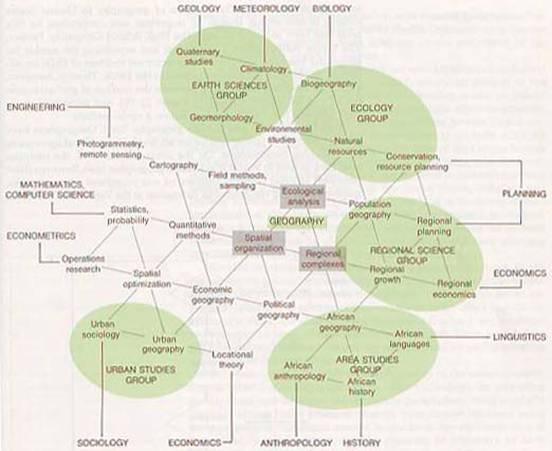
\includegraphics[width=.7\linewidth]{haggett1975_p587.jpg}
    \end{sidecaption}
  \end{figure}

Une exposition des influences de l'écologie, et des sciences naturelles (voir également le schéma plus général proposé par Haggett en 1975 \ref{fig:I_geoLink}), que l'on retrouve neaucoup plus détaillé dans l'étude de l'écologiste et géomorphologue \textcite{Stoddart1967} parue en 1967.

Pour le moment, et c'est aussi le cas dans les précédents ouvrages de ces pionniers, seules des tentatives probabilistes sont évoquées, via les travaux d'Hägerstrand, ou des économistes comme Curry. La méthode hypothético-déductive héritée des premiers géographes théoriciens semble encore être un implicite à la construction et l'évaluation des modèles. Les idées fortes de la systémique semblent avoir été entendues, mais paradoxalement il n'y a quasiment aucune référence à cette période aux techniques mathématiques ou informatiques capables d’opérationnaliser un tel système, et aucune application réelle. \autocite[467-468]{Harvey1969}

\paragraph{Les pionniers de l'opérationalisation systémique en Europe}

La génération suivante de géographes va jouer un rôle important dans l'opérationnalisation de ces concepts au début des années 1970, tant en Angleterre, qu'en France où les géographes développent en collaboration avec des mathématiciens et physiciens les aptitudes nécessaire à la manipulation de ces nouvelles techniques computationnelles. \autocite{Pumain2002} 

\hl{Il manque Chorley, voir article cybergeo sur le sujet + le travail de Varenne qui fait une analyse de ce courant en détail}

En Angleterre, la planification est issue d'une tradition qui date pour le \textit{Regional Planning and Policy} d'après 1920, et pour le \textit{Land use planning} d'après 1930. Ces activités sont rapidement construites en relation étroite avec les universitaires, les ingénieurs et les politiques publiques \autocites{Bennett2003}[727]{Davies1997}; un existant qui va être bouleversé courant des années 1960-70 par la rencontre conjointe des développements théoriques systémiques, des modèles de planification américains du milieu des années 1950, et d'une littérature qui anticipe la vague systémique. \autocites[4-8]{McLoughin1985}[253]{Batty1978} \footnote{\foreignquote{english}{The quantitative revolution in geography as encapsulated in books such as Peter Haggett's (1965) Locational Analysis in Human Geography, the various special issues of the Journal of the American Institute of Planners on traffic (1959) and land-use models (1965), books on the post-industrial structure of cities such as Explorations into Urban Structure (1964) all bolstered and anticipated the systems approach. The second edition of Stu Chapin's Urban Land Use Planning in 1965 was also a land mark in the changing conception of planning in America.}}

C'est sur ce substrat \autocite[253]{Batty1978} que des auteurs comme McLoughlin ou Chadwick publient dès le courant des années 1960 des états de l'art et des manuels d'applications qui vont rester pendant presque dix ans des références pour repenser la planification urbaine sous l'angle nouveau de la systémique \autocite[719]{Davies1997}. Une période qualifiée d'âge d'or pour la systémique anglaise, qui même si elle dure peu de temps \autocites[726-727]{Davies1997}{McLoughin1985}, marque toute une jeune génération de planificateurs qui vont être profondément influencés par ces approches \autocite[256]{Batty1978}; un constat alors en complet décalage avec la situation américaine, qui cristallise comme on a pu le voir dans la section \ref{ssec:crise_mutation} l'échec d'une décennie déjà révolue; les nouvelles pratiques, les nouveaux modèles ayant déjà exfiltrés les Etats-Unis, et la nouvelle génération bricolant déjà les meilleurs modèles en vue de les améliorer. C'est dans ce cadre notamment que le physicien et planificateur Wilson publie en 1970, le résultat de 4 ans de travail pour concrétiser son idée, passer du paradigme newtonien au paradigme statistique Boltzmanien pour revisiter dans une version spatiale et dynamique les modèles numériques classiques américains. \autocite{Wilson2010} Une approche qui va devenir avec le temps \enquote{l'école entropique} comme la nomme \textcite{Guermond1984}.

De cette plus jeune génération, à la croisée de ces inspirations, et tout à fait conscient des errements passés \footnote{Voir la conclusion de l'ouvrage de \textcite[357]{Batty1976} ou l'auteur fait le point sur ces différentes positions, toutes abordées en filigramme dans ce livre synthèse : prédiction, explication, éducation }, on trouve des chercheurs maniant parfaitement ces techniques hybrides. Michael Batty est un bon exemple de chercheur représentatif de cette synthèse, qui pressentent l'urgence de s'engouffrer dans une modélisation spatialisée plus dynamique \autocite{Batty1971,Batty1972} appuyée par les mathématiques des systèmes dynamiques, que cela soit au travers du vocabulaire de la dynamiques des systèmes de Forrester, ou en suivant la toute nouvelle voie des modèles dérivées de l'école entropique de formation par Wilson.

%Le canal en écologie et géographie physique, dans la lignée des travaux de Chorley va également être particulièrement influent, avec l'avénement de modèle opérationel dérivée de la dynamique des populations de Lotka. \autocite{Batty 1971 ou 1972 ....}

%On trouve une analyse des premier essai systémique de Chorley analysé par le prisme des proposition du découpage de Parsons dans l'essai de Gregory. 

Comme déjà évoqué brièvement à la fin de la section \ref{sssec:realite_neopositiviste}, les géographes français semblent au début des années 1970 peu réceptifs à l'épistémologie néo-positiviste, et beaucoup plus concentrés sur l'apport des nouvelles méthodes quantitatives dont la substance est révélée brutalement aux géographes français par la lecture (et ensuite la traduction) de manuels anglo-saxons qui condense déjà 15 ans de pratiques et de découvertes \autocite[129]{Pumain2002}.

Concernant la diffusion du paradigme systémique \footnote{Le cas de la diffusion des méthodes quantitative en France et de sa structruration en réseau de chercheurs fait actuellement l'objet d'une thèse, mené par Sylvain Cuyala et dirigé par Marie-Claire Robic, Denise Pumain.}, les recherches d'Olivier Orain \autocite{Orain2001} sur ce sujet sont précieuses. L'auteur nous propose de lister dans les embranchements intellectuels d'une discipline en pleine reconstruction, les convergences et divergences autour de l'acceptation de concepts dont Orain estime qu'ils se sont diffusés dans la géographie française au début des années 1970. La diffusion de la GST de Bertalanffy est renforcée par la publication en 1973 de son ouvrage principal, alors même que l'activité conjointe (publications, traductions, organisations de conférences, d'ateliers) de différents passeurs ayant séjourné à l'étranger comme Bernard Marchand, Wanda Herzog, Henri Reymond, Jean-Bernard Racine, Sylvie Rimbert est soutenue par des acteurs \enquote{installés} comme Philippe Pinchemel, Paul Claval, Roger Brunet, Charles-Pierre Péguy \autocite{Pumain2002,Cauvin2007}, déjà au fait des publications et techniques pionnières anglo-saxonnes. 

Le mot \enquote{système} sort de l'ornière du sens commun et se pare de nouvelles significations, sous l'effet nottament d'ouvrage de référence comme celui de Jean-Bernard Racine et Henri Reymond  \textit{L’Analyse quantitative en géographie} (1973). Premier livre de géographie quantitative en France \autocite{Cauvin2007}, il développe un \enquote{ [...] vibrant plaidoyer pour le développement de concepts et de méthodologies systémistes dans une discipline qui selon eux, \enquote{ découvre que la notion de système lui était depuis longtemps familière, comme la prose à Monsieur Jourdain, et qu'il ne lui manquait que de la formaliser pour la rendre opérationnelle.}} \textcite{Orain2001}. Un appel qui sera entendu semble-t-il, pour Orain \autocite[23]{Orain2001} une des explications pour comprendre le succès connu par la systémique fin des années 1970 début 1980 est le fait que \enquote{[...] les Nouveaux Géographes [...] ont trouvé dans l’idée de système un appareil conceptuel permettant à la fois de penser l’intégration de l’hétérogène et d’apporter une légitimité scientifique à l’étude de la région} 

\Anotecontent{etat_artDPMC}{Sur cette thématique on trouve un excellent récit de Denise Pumain et Marie-Claire Robic \autocite{Pumain2002}, ou de Colette Covin \autocite{Cauvin2007}}

Dans l'établissement d'une géographie systémique, le Groupe Dupont qui nait à la suite de la conférence \enquote{révélatrice} donnée par Marchand en 1970 s'avère être un creuset important pour la formation, la réflexion, l'échange intra/inter-disciplinaire, et l'expérimentation autour de ces nouvelles techniques \autocites[2]{LeBerre1987}[125-128]{Pumain2002}. Une structure d'accueil que l'on imagine nécessaire pour fédérer des jeunes géographes plus habitué à l'étude monographique qu'à l'utilisation d'outils computationnels. Une période 1971-1975 marquée par la volonté des \enquote{nouveaux géographes} de se former aux mathématiques, une étape absolument nécessaire pour tirer profit par la suite de ces nouveaux formalismes statistiques et informatiques. \Anote{etat_artDPMC}

En terme de réalisation, différentes écoles vont se créer autour d'objet géographiques ou de techniques parfois différentes, mais avec la même volonté de rendre compte de la complexité des systèmes géographiques en usant des outils mis à disposition par ce nouveau paradigme systémique. 

Durand-Dastès et Auriac sont des exemples de géographes qui développent dans leurs études toute la puissance heuristique des concepts systémique et de leur traduction graphique pour décortiquer la complexité des systèmes géographiques.

Une autre branche de géographe va pousser cette démarche heuristique encore plus loin, en lui donnant corps dans des modèles de simulation. C'est le cas par exemple du projet A.M.O.R.A.L (\hl{Signification terme}) réalisé par des géographes et informaticiens Grenoblois \autocite{1984}, qui est un des premiers résultat d'approche systémique spatialisé ayant pour objet d'étude une région française. Un double enjeu et une double expérience ici pour ces géographes, qui décident de tester la méthode systémique en la déroulant dans sa totalité, ce qui signifie également pour les étapes de réalisation de collaborer avec des informaticiens sur la partie systèmes dynamique. \autocite{Guermond84, LeBerre1987}

\Anotecontent{exp_amoral}{\enquote{[...] mes premières tentatives de modélisation systémique sont liées à un événement conjoncturel : la rencontre de chercheurs en informatique qui travaillaient, dans l'esprit de la dynamique de système de J.W. Forrester, à la mise au point d'un nouveau langage de simulation. Ils cherchaient à identifier, pour les formaliser, les types de problèmes soulevés par les recherches appliquées. Le groupe de géographes grenoblois avec lequel je travaillais, séduit par quelques ouvrages sur l'approche systémique, était tout prêt à faire l'investissement intellectuel pour tenter son expérimentation en géographie. C'est ainsi que nous avons choisi de modéliser la dynamique de l'emploi dans le système urbain de la région Rhône-Alpes.} \autocite[8]{LeBerre1987}}

Dans le cas du modèle A.M.O.R.A.L ( Analyse systémique et MOdélisation des ALpes ) \autocite{Durand1983}, la démarche poursuivie est explicitement\Anote{exp_amoral} celle de l'expérimentation de l'\enquote{approche systèmes dynamiques} \autocite{Rosnay1975} à l'étude de la région, avec en tête des modélisateurs la réalisation de multiples objectifs, à la fois d'apprentissage, d'amélioration (prise en compte du spatial), de faisabilité, et d'applicabilité décisionnelle.

\Anotecontent{it_allen}{\enquote{Mais la rencontre opérationnelle - décisive -je l'ai faite en 1982, en allant à Créteil écouter - ne me demandez pas pourquoi - un colloque sur l'entropie dans lequel Peter Allen faisait un exposé sur les théories de l'auto-organisation. Dans cet exposé, il décrivait les modalités de changement de ces systèmes ouverts, loin de l'équilibre, qui connaissent de multiples fluctuations, dont certaines pouvaient s'amplifier et contribuer à modifier la structure du système tout autant que certaines bifurcations externes. C'était exactement ce que j'avais observé en étudiant les recensements périodiques de population, en poids économique, et transformaient leur structure qualitative sur le plan de leur portefeuille d'activités économiques, sur le plan de leur composition sociale, tout ceci en lien, bien sûr, avec des représentations que nous avions de cette dynamique des villes en terme d'images de marque, d'attractivité pour les migrations, etc.
Tout de suite j'ai été séduite par cette approche, et j'ai essayé d'expérimenter avec ces modèles mis au point par Peter Allen, qui à l'époque travaillait encore dans le laboratoire de Prigogine à Bruxelles avec Michèle Sanglier, mais plus particulièrement en direction d'applications à l'économie et à la géographie.[...] Il élaborait en effet des modèles spatialisés, nottament un modèle dynamique intra-urbaine ou intrarégionale [...]; il y'avait là beaucoup d'éléments de théories géographiques qui étaient mis dans un modèle de simulation qui permettait d'expérimenter les effets de ces briques théoriques et de les confronter à des observations.} \autocite[153-154]{Schmid2014}}

\Anotecontent{appli_allen}{\enquote{Tous ces auteurs se sont toutefois heurtés insuffisante prise en compte de la dimension spatiale dans cette famille de modèles. Aussi, des travaux application et élaboration de \textit{modèles urbains} qui soient à la fois \textit{dynamiques et spatiaux} sont en cours. Un modèle comme celui de P.Allen (1978), fondé sur l'analogie des structures dissipatives en physique, permet de simuler le développement d'une ville en tenant compte des interactions non linéaires (avec effets d'amplification ou de saturation), spatiales ou non spatiales, qui commandent la redistribution des emplois et des populations entre les différents quartiers. Il permet de prévoir diverses configurations possibles dans le futur à partir d'une histoire donnée. Ce modèle a été appliqué à la simulation du développement de agglomération de Rouen (Ozan et al. 1983)} \autocite{Pumain1983}}

\Anotecontent{auto_definition}{Un autre concept important est introduit par Ashby dans le mouvement Cybernétique, l'introduction du mot \enquote{auto} amorcent un virage réflexif propre à la seconde Cybernétique, piloté par William Ross Ashby et Von Foerster. Si le concept en lui même est largement intuité dans les thèses de Goethe et Bertalanffy \autocite[102]{Pouvreau2013} dans sa traduction biologique, on retrouve un concept équivalent dans le \enquote{order-from-noise} de Von Foerster, et \enquote{order-from-fluctuation} dans la physique de Prigogine.}

De façon parallèle Denise Pumain, aidé par d'autres géographes comme Léna Sanders et Thérèse Saint-Julien participe dès 1980 d'un courant \autocite{Pumain1983, Pumain1984, Pumain1989} qui vise l'application des modèles de simulation à l'étude des villes et des systèmes de villes, et cela sur des bases beaucoup plus empiriques, devançant ici les diverses tentatives des anglo-saxons faites jusqu'à alors \autocite[99-100]{Pumain1989}. Mais dans le cas de cette équipe, si l’intérêt porté à la dynamique des systèmes de Forrester est là aussi évidente \autocite{Pumain1983, Pumain1984}, le chemin emprunté sur le plan opérationnel va semble t il rapidement divergé de celui suivi par l'équipe AMORAL. 

Une fois la révélation d'une opérationalisation possible par l'usage de la \enquote{dynamique des systèmes}, les géographes peuvent donc aller plus loin dans l'exploration du support mathématique sous-jacent, et ainsi mesurer dans l'évolution des \enquote{systèmes dynamiques} vu comme discipline mathématique la possibilité de construire des modèles encore plus proches d'une évolution réelle des objets géographiques.

Ainsi, là ou AMORAL cherche à spatialiser l'approche systémique qui dérive de la dynamique des systèmes de Forrester, les frustrations de l'équipe de Denise Pumain face à leur propres études passés sur la dynamiques des villes vont les amener à explorer un tout autre chemin en terme d'opérationalisation.

A l'origine ce sont deux conférences qui amène Denise Pumain à intégrer l'univers systémique à ses analyses, \enquote{la première organisée à Boston au MIT en 1981, encore très largement dominée par l’analyse de systèmes de type Forrester, et la seconde à Bruxelles en 1982 (AFCET, SOGESCI, 1982) déjà largement consacrée aux théories de l’auto-organisation.} \textcite[27]{Pumain2003} \autocites[27]{Pumain2003}{Schmid2014} 

\hl{transition ici maladroite}
Mais en réalité, ce n'est pas tant l'évolution des concepts qui comptent pour les géographes mais leur définition en terme opérationnels dans les modèles de simulation \autocite{Pumain2003}, seul moyen de confronter les données récoltés à ces nouvelles formes d'explications mathématiques. Bertalanffy entre autre l'avait déjà bien compris, sans réelles démonstrations les hypothèses intuitées, même lorsqu'elles sont quasi certaines, ne sont tout au mieux pour les autres chercheurs que des aides à la réflexions. Ainsi, et c'est avec une rapidité presque déconcertante, qu'il se raccroche aux premières découvertes de Prigogine en 1946 sur la physique des systèmes ouverts loin de l'équilibre pour appuyer ce qui jusque là ne sont que des intuitions dans sa théorie organismique, et qui forme le prélude à un projet systémique plus général (voir Annexe A pour plus de détail).

Ainsi, et c'est dans ce contexte de frustration par rapport aux approches existantes \Anote{appli_allen} que se produit au début des années 1980 cette découverte contingente du concept d'auto-organisation, dont la réalité opérationnelle exprimés dans des modèles mathématiques exposé par les physiciens de l'école de Bruxelles semble offrir tout à coup toutes les garanties pour former des modèles de simulations beaucoup plus réalistes de l'évolution des villes. \Anote{auto_definition} \autocite[350]{Pumain1998a} La possibilité également de concrétiser les intuitions systémiques des pionniers qui envisage très tôt la nécessité de penser les systèmes urbains comme des systèmes ouverts, comme celle évoqué en 1964 par \textcite{Berry1964a} et son article \enquote{Cities as systems within systems of cities}. La rencontre de Denise Pumain avec le chimiste  Peter Allen en 1982 à Créteil \Anote{it_allen} est l'expression même de cette contingence, qui va donner par la suite naissance à de multiples modèles et collaboration avec les physiciens de l'école des \enquote{structures dissipatives} de Bruxelle d'abord, puis de l'école de la \enquote{Synergétique} de Haken ensuite. \autocites[27]{Pumain2003}{Pumain1982b, Schmid2014}. 

A une phase cybernétique déjà révélatrice de concepts systémiques tout à fait nouveau pour penser la causalité en géographie, les géographes découvrent par extension la richesse et la pluri-disciplinarité de cette discipline des systèmes dynamiques, alors en pleine évolution. Ainsi, déjà évoqué par Poincarré au début du siècle, la remise au goût du jour des théories de la bifurcation introduit la possibilité d'un changement qualitatif exprimé dans la topologie de trajectoire. 

\begin{framewithtitle}{Les théories de la bifurcation}

	% \begin{figure}[h]
	% \begin{sidecaption}[fortoc]{Un exemple de bifurcation Pitchfork}[fig:S_BPF]
	%   \centering
	%  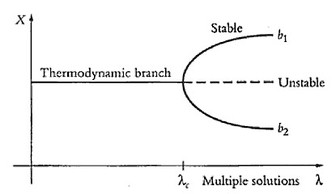
\includegraphics[width=.7\linewidth]{pitchfork_bifurcation.jpeg}
	%   \end{sidecaption}
	% \end{figure}

\end{framewithtitle}

%La théorie des catastrophe de René Thom, bien connus des géographes, est un cas particulier de la théorie des bifurcations.

Elle offre un support aux découvertes des physiciens engagé depuis les années 30 dans les travaux sur les processus physique et chimique des systèmes ouverts éloignés de l'équilibre, qui observe dans la trajectoire d'évolution de ces systèmes l'apparition de zone d'instabilité, causé par la modification en interne des fluctuations ou en réponse à des variations des échanges externes avec l'environnement. 

Si certaines conditions d'une auto-organisation avait déjà avancé dans une preuve matérielle ( Homéostat ) et un support théorique (Loi de la Variété requise) dans les travaux par exemple d'Ashby \autocite[800-801]{Pouvreau2013}, les physico-chimistes comme Prigogine ou Haken, en montrant qu'il était possible dans certains systèmes physique (laser) ou chimique (structures dissipatives) chaotique, de voir apparaître au cours des bifurcations de nouveaux équilibres dynamiques caractérisés par l'émergence de structures ordonné de niveau supérieur issue de l'organisation des interactions à un niveau inférieur, ont fournit une évolution du substrat théorique et mathématique solide du concept d'auto-organisation sur lequel peuvent s'appuyer les chercheurs pour expérimenter des analogies dans les systèmes sociaux ou biologiques.

%l'approche d'un point de bifurcation correspondant à l'émergence d'une structure lié à une variation de paramètres dans un processus chaotique/instable décrivant une trajectoire stable entraînant l'émergence imprévisible d'un nouvel état ordonné/stable, dont la structure est maintenu par consommation d'énergie extérieure.

%dévoile de nouvelle perspectives pour penser l’emboîtement et les relation opérant entre les différentes échelles d'observations (voir Annexe A).

%La matérialisation d'un modèle urbain, même théorique, ouvre la voie à des développements qui ouvre la voie à une nouvelle forme de causalité.

La translation de ces concepts sera opérés avec précaution par Pumain et Sanders, et amène une réflexion sur l'évolution des objets géographiques dont on trouve une plus grande explication dans les textes de \textcite{Pumain1982b, Pumain1989}.


L'apport du paradigme systémique, et de son opérationalisation 

Sous détermination
Equifinalité

%Les deux approches sont clairement supportés par une double dialectique dans l'utilisation des outils statistiques et systémique, et dans la déduction et l'induction. (hum)


%\enquote{Tenant pour légitime de traiter les êtres vivants et leurs associations comme des systèmes physiques, Lotka insistait toutefois sur le fait qu’il s’agit de « systèmes ouverts » aux flux de matière et d’énergie (ainsi que Raymond Defay (en 1929) et Bertalanffy (en 1932) les qualifièrent plus tard), capables d’échapper à l’équilibre thermodynamique défini par un maximum d’entropie promis aux systèmes fermés par le Second Principe, et d’évoluer vers une structuration croissante.}\autocite{Pouvreau2013}

%\autocite{Pouvreau2013} sa théorie arrive à maturation : \enquote{Un système organique quelconque n'est essentiellement rien d'autre qu'un ordre hiérarchique de processus qui se tiennent mutuellement en équilibre de flux [...] Un organisme vivant est un ordre hiérarchique de systèmes ouverts, qui se maintient sur la base de ses conditions systémiques par un changement de ses composants}

L'apport de ces techniques, est un vrai écho à ce que disait Le Berre; Sanders et Pumain. D'une part les outils permettent d'ouvrir de nouvelles perspectives de réflexions, et ceux ci s’intègrent dans une chaîne de raisonnement qui s'organisent non pas de façon linéaire mais dans dialogue ou ce sont les usages, les questions, les objets à étudier qui guident l'utilisation et l'amélioration de ces outils.

% Partant de Pumain2002 Pumain2003, la première remise en cause de la causalité est le concept de non linéarité des interactions, 

Sachant la vision de la validation dominante dans les années 1970, le tournant systémique  Ces deux moments viennent remettre en cause la construction et l'évaluation des modèles en géographies, et sont détaillés par la suite.

% Relation de variété entre les niveau de hierarchie, augmentation du degré de variété, ce qui va avec le concept équifinalité, un peu different du concept de sous détermination... 
% Plusieurs débats qui vont venir agiter la problématique de la construction des modèles, et surtout de leur validation.
% Forrester causalité, construction des modèles, sous détermination 
% Auto-organisation problématique de  

\subsection{Les problèmes de la Validation}
\label{sec:validation}

%Dans cette partie, il s'agit donc de mettre en avant ces débats philosophiques en les reliant aux nouvelles problématiques de construction des modèles tel qu'elle apparaissent aux tournant des années 1970.

%Quel sont les moyens offerts de cette validation ? Existe-il une spécificité de cette validation dans son application en science sociale, et plus spécifiquement en géographie, et qui n'est pas prise en compte dans ces définitions ?

%Plusieurs débats viennent encadrer à la fois la validation mais aussi le support opérationel de cette validation. Autrement dit, comment détermine t on si un modèle est validé ou pas, et quel est la nature de cette validation opère sur un substrat particulier, qui en fait une expérience sur le réel de second ordre.


Necessite d'avoir une validation pour les sciences sociales.
IMPORTANT

L'apport de nouvelle techniques vient remettre en cause le schéma classique de validation principalement porté par Naylor.

\subsubsection{L'impact du \enquote{programme Forresterien} dans le débat sur la Validation}

Deux dates sont à retenir dans le programme Forresterien, la publication du \enquote{programme} d'\textit{Industrial Dynamics} en 1961; aboutissement des recherches démarrés en 1956 au MIT, et dans un deuxième temps en 1969 la proposition de translation de ce programme à l'étude plus large des systèmes sociaux, avec l'expérience du modèle \textit{Urban Dynamics}.

Pourquoi parle-t-on de programme ici, et non pas seulement de modèle ? 

L'apport de Forrester ne se résume pas en réalité au seul nouveau langage de programmation DYNAMO, celui ci propose aussi avec une méthodologie et un vocabulaire graphique. Trois éléments qui une fois réunis permettent de dériver opérationnelement les concepts clef du projet systémique dans un modèle de simulation dynamique, ce qui en fait un outil d'intérét général non seulement pour la géographie, mais pour toute les autres disciplines confondues (biologie, économie, sciences humaines, etc.) \autocite{Rosnay1975}

\paragraph{Urban Dynamics dans le contexte géographiques des années 1970}

Provenant d'une toute autre inspiration et construit selon un tout autre patron que les modèles urbain réalisé jusqu'à la fin des années 1970, le modèle \textit{Urban Dynamics} de \textcite{Forrester1969} fait une entrée très remarquée dans le milieu des \textit{policies}. Celui met en jeu une ville abstraite et isolée, non-spatialisé, ou interragissent de façon a-spatialisés de multiples mécanismes regroupés par activités et organisés en chaine causale. Le modèle ne fait appel à aucune données pour calibrer ou vérifier les sorties générées, et à ce titre il ne peut pas être considé comme un modèle décisionnel sérieux pour les \textit{policy analysis} de l'époque. \autocite{Lee1973}. Soumis à une très forte médiatisation pour l'époque, les critiques sur le modèle se font parfois vives tant du coté des citoyens \autocite{Forrester1989, Forrester2007} que des universitaires géographes \autocite{Tobler1970a, Berry1970, Batty1971}.

Il est vrai que d'un point de vue purement géographique et même technique, le modèle \textit{Urban Dynamics} n'introduit pas tant d'originalité par rapport aux éléments acquis par la rencontre entre la vision d'Hägerstrand et les pionniers universitaires 10 ans auparavant; on se remémorera à ce sujet la citation de \textcite{Morril2005} qui résume très bien l'importance de cette convergence, ici en quatre grands points : \foreignquote{english}{First was the introduction (at least at the geography) of the idea of spatial and time-processes, that geographic development over time could be understood and modeled; second was the particular processes of spatial diffusion; third was the technique of Monte-Carlo simulation; and fourth was the idea that individual behavior, not just that of large groups, could be modelled}. Ainsi après tout, les premiers modèles de simulation qui implémente la dimension temporelle, stochastique, dans le premier langage Fortran, sont datés d'avant 1965, et dépasse par bien des aspects la vision a-spatiale proposé par Forrester.

L'étude des processus de diffusion abordé dans les simulations pionnières suppose assez naturellement que les géographes intégrent le temps dans leurs analyses, et il a été vu précédemment que la simulation est un formidable outil d'expérimentation pour la projection et l'évaluation dans le temps de multiples hypothèses (section \ref{ssec:labo_virtuelle}). En dehors de quelques exceptions - dont on trouve une liste comparative réalisé par \textcite{Batty1972} incluant entre autre la gestion de l'espace, du temps, et la nature des dynamiques \footnote{Le modèle TOMM (Time Oriented Metropolitan Model) de Crecine, le modèle EMPIRIC, les travaux de Paelinck, ou encore de Wilson qui adapte les travaux existants en démographie, ou hérités de la dynamique des populations en écologie/biologie} - pourquoi cette approche percole t elle aussi lentement dans l'analyse des systèmes urbains en géographie, où la simulation numérique est mobilisé à la même période sans pourtant y intégrer la dimension temporelle. Sorte de principe de parcimonie poussé à l'extreme, ou l'absence du temps si elle permet de simplifier l'analyse, mène toutefois à des prédictions absurdes ou impossibles, qui ne tiennent pas compte des évolution de structures sur lesquels s'appuient les interactions dans les systèmes urbains. Le constat d'une forme d'auto-censure de la discipline pour lequel \textcite[296-297]{Batty1976} nous donne quelques pistes de compréhensions sur lesquelles il nous faudra revenir (\hl{section à appeler}) : 

\foreignquote{english}{There are, however, good reasons why the comparative static approach has been widely applied. The status of theory in urban economic and geographic systems with regard to time is almost non-existent. [...] Yet there are severe problems in trying to develop dynamic theory, two of which are worthy of some discussion.[...]

Perhaps the major problem concerns the ability to observe or monitor the urban system. Unlike the physical sciences in which the effect of critical variables on the system of interest can be isolated in the laboratory, such a search for cause and effect is practically impossible in social systems. Thus, there are many instances when it is difficult, if not impossible, to disentangle one cause from another in the changing behaviour of such systems. This is a fundamental limitation which is referred to here as the observational dilemma.

A second problem concerns that hoary perennial data. [...] data are often difficult to assemble for one cross-section in time, and the collection of time series data is usually a formidable and sometimes infeasible undertaking. Furthermore, such data often become less consistent and sparser as earlier time periods are needed and, frequently, the time periods between points at which data have been collected, are too large to be useful for dynamic modelling}

Si on revient au modèle \textit{Urban Dynamics} de Forrester, celui ci pourrait après tout passer pour une nouvelle tentative parmis d'autres, car comme Tobler le fait remarquer dans sa critique du modèle : \foreignquote{english}{In other words, it is a classical non-linear deterministic equilibrium model, but of great complexity.} \textcite{Tobler1970a}

Pourquoi Batty en fait il alors régulièrement un modèle pivot dans son argumentation \textcite{Batty1971, Batty1976, Batty2001, Batty2008} dans l'évolution de la discipline, et pourquoi celui ci a t il autant attiré l'attention dans le monde académique ?

Sur ce deuxième point, on a déjà donné un élément de la réponse dans l'introduction. Forrester vient avec plus qu'un modèle, il vient avec un programme qui embrasse littéralement les concepts de la systémique \autocite{Berry1970}, ce qui permet d'apporter, avec l'intégration du temps, un nouveau point de vue sur la planification et la mise en place des politiques publiques. Ainsi malgré ses défaut, \foreignquote{english}{[...] the model is an illustrative first attempt that points the way for others. It is the direction that is important, and Forrester's book may yet prove to be one of the important signposts in the attempt to deal more sensitively and effectively with urban problems.} \autocite{Berry1970}

L'autre point fort du programme de Forrester est la possibilité d'opérationnaliser ces concepts de la systémique tout en maintenant un coût d'accès à la simulation qui parait plus adapté au monde académique des sciences humaines et sociales, et cela entre autre par la mise en place d'une triple entrée en la matière : informatique avec DYNAMO (un langage déjà orienté pour la simulation), mathématique avec les systèmes dynamiques et graphique avec les diagramme de \enquote{stock and flow}. 

Pour ces deux raisons, on comprendra donc ici que le monde académique soit plus intéressé par les nouvelles possibilités offertes par l'environnement support du modèle que par le modèle en lui même, qui restera chez les géographes un cas d'utilisation finalement assez peu repris dans des travaux ultérieurs chez les anglo-saxons \autocite[308]{Batty1976}, et chez les français. \hl{(ref)}

Ainsi, ce n'est pas tant sur les aspects temporels que Batty en fait un modèle en rupture avec son passé, mais sur le débat qu'il soulève du point de vue de la validation.

Pour comprendre la position de Forrester sur ce point il faut s'intéresser d'un peu plus près à sa vision de la modélisation et à l'utilisation qu'il souhaite en faire dans le cadre des politiques publiques. Pour lui, le problème n'est pas tant les données, dont on finit toujours par les obtenir, \foreignquote{english}{ [...] but rather inability to perceive the consequences of information we already possess.}. Les gens mobilisent pour l'interprétation des données des modèles mentaux, hors souvent ils se trompent, et les conséquences de leur intuitions amènent alors à constater la faillite des politiques ainsi menés. Pour \textcite{Forrester1971}, l'usage de modèle de simulation permet de re-projeter ces modèles mentaux faillibles sur des modèles informatiques dont la construction nécessite la formulation d'hypothèses de façon plus explicite, plus compréhensible, et sur lequel il est possible de dialoguer de façon plus constructive. Il n'est plus question de choisir fonction d'un seul scenario, mais de plusieurs, avec la possibilité de projetter et d'évaluer dans le temps les conséquences de dynamiques complexes sur un système simplifié envers un objectifs donné, et cela avec la garantie d'une fiabilité bien au delà de ce le seul esprit humain ne pourrait espérer. Avec souvent un résultat sans appel, \foreignquote{english}{[...] behavior is different from what people have assumed.} Un comportement qu'il arrive à démontrer par le jeu des rétro-action des mécanismes de son modèle \textit{Urban Dynamics}, qui illustre les effets tout à fait contre-intuitifs de certaines politiques publiques.

En réalité on comprend beaucoup mieux la démarche de Forrester dès lors qu'on comprend qu'il n'a jamais été question ici de faire un modèle opérationel \autocite{Batty2001}, ce qui explique entre autre la perplexité des planificateurs ayant investit des millions de dollar dans la construction de modèles s'appuyant sur des récoltes de données couteuse et fastidieuses.

Le support de cette discussion passe par l'établissement d'un graphe causal représentatif d'un système clos dans sa définition, mais ouvert dans ses échanges vers l'extérieur, dont les éléments et les interactions entre les éléments sont au centre du débat. \hl{description graphe forrester}

Mais en acceptant cela, et compte tenu de l'\textit{observational dilemna} définit par Batty, le modèle de simulation devient dans l'établissement de sa structure causale la projection d'une histoire, d'un point de vue, ici celui de Forrester et de ses collaborateurs. Dès lors l'attention ne se porte plus seulement sur le résultat, mais aussi sur le bien fondée des hypothèses mobilisés par Forrester pour établir ce résultat. 

Il ya un certain paradoxe à voir dans cette situation, car si effectivement Forrester donne à voir son raisonnement, contrairement à de nombreux modèles urbains autrefois qualifié de boite noires, c'est justement sur ce point qu'il va se faire attaquer. Les critiques des géographes ne manquent pas alors de rapeller qu'en dehors de l'a-spatialité et l'isolation du modèle, celui ci n'a intégré absolument aucune référence aux théories urbaines dans son travail. Outre le fait que ce n'est pas très fair play pour les universitaires, cet isolement relatif (Forrester mobilisera d'autres sources) se traduit dans le modèle par la mise en oeuvre de centaines d'hypothèses (400 équations, 300 variables et paramètres \autocite[63]{Pumain1989}), difficilement justifiables ou testables de façon empirique pour la plupart. \autocite[307]{Batty1976}

La critique de \textcite{Tobler1970a} sur ce point est explicite, \textit{Urban Dynamics} \foreignquote{english}{[...] is a classical non-linear deterministic equilibrium model, but of great complexity. Herein lies its importance for it is rather grandiosely conceived. [...] Not only the values of the parameters, but also which variables are chosen for consideration and how they are interconnected, are critical. [...] the danger is that his model has not really been tested empirically, thus the policy implications may be wrong, and the model - because of its complexity - is extremely difficult to test. A very careful study of the many assumptions of the model are required. Also required are more competing models, thus the book’s greatest achievement may be the competition which it stimulates.} 

Dernier point, peut être le plus préjudiciable, est la règle donné par Forrester pour définir le choix des hypothèses dans un graphe de causalité : 
\foreignquote{english}{Formulating a model of a system should start from the question \endquote{Where is the boundary, that encompasses the smallest number of components, within which the dynamic behavior under study is generated?} [...] In concept a feedback system is a closed system. Its dynamic behavior arises within its internal structure. Any action which is essential to the behavior of the mode being investigated must be included inside the system boundary.} \autocite{Forrester1968b, Richardson2011}

\Anotecontent{lee_forrester}{\foreignquote{english}{He removed about two-thirds of the model without altering the remaining parts, which were left intact, and the model performance was not significantly altered.}\textcite[176]{Lee1973}}
\Anotecontent{batty_forrester}{\foreignquote{english}{An interesting, fruitful and amusing piece of work has been undertaken by \autocite{Stonebraker1972} who has simplified the model drastically by reducing the total number of model equations by two-thirds. The results of running the model in this fashion are much the same as Forrester's and this has led Smith and Sage (1973) to propose the use of hierarchical system theory as a tool for simplifying the model.}\autocite[308]{Batty1976}}

Sachant cela, le fait que différentes équipes arrivent à reproduire la même dynamique finale avec la mise en oeuvre de modèles beaucoup plus parcimonieux est catastrophique pour l'argumentation de Forrester ! Lee \Anote{lee_forrester} et Batty\Anote{batty_forrester} font référence en particulier aux travaux de \autocite{Stonebraker1972}.

Ainsi Batty fait référence à Forrester non pas pour éclairer sa réussite dans la lourde tâche de fabriquer un modèle crédible sur le plan des hypothèses du point de vue d'une communauté, car sur ce point l'échec est complet.

%deux paragraphes ci dessous a bouger ailleurs ?
Aussi pour \textcite{Batty2001}, le risque pour des modèles n'impliquant pas la vérification par les données (sur les hypothèses, mais aussi en sortie) de tomber dans une situation similaire à la \foreignquote{english}{Forrester strategy}, identifié par \textcite[7-8]{Batty2001} comme le retranchement des modélisateurs dans une rhéotique masquant en réalité une absence de volonté ou une incapacité (technique, méthodologique) à justifier de la chaîne causale mise en place dans le modèle, celui ci ne servant plus qu'à animer ou illustrer un débat où clairement la neutralité scientifique n'est plus une priorité.

On se retrouve avec un problème insoluble, avec d'un coté cette nécessité -pour être crédible d'un point de vue scientifique - de pouvoir justifier empiriquement le réseau hypothèses mobilisés dans notre modèle complexe, et d'un autre coté l'impossibilité de pouvoir toute les justifier du fait de l'\textit{observational dilemna} et de la difficulté/impossibilité d'obtenir des données dans nombre de science sociale.

Perhaps the clearest model which broke from this tradition and which illustrated distinctly the problems posed by the current generation of models based on complexity was Forrester’s (1969) Urban Dynamics model.\autocite{Batty2001}

%Car comment valider un modèle qui ne s'appuie sur aucune données autres que des valeurs de paramètres, et qui évoque des conclusions sans avoir été calibré au préalable ? Comment discuter des résultats de cette longue suite d'hypothèses reliés les uns aux autres par des interaction complexes, difficile ou impossible à vérifier empiriquement ? On retrouve là les deux points évoqués par Batty pour justifier du retard dans l'intégration du temps dans les modèles urbains, sur lesquels Forrester est clairement mis en difficulté.


\paragraph{La confrontation entre deux approches de la Validation}
\label{p:confrontation_approches}

Dès la publication d'\textit{industrial dynamics} des critiques extrémement vive remettent en cause la scientificité de son modèle, certains opposant à sa méthode de validation celle plus binaire tel que proposé par Naylor, un des pionniers dont la vision à une large influence dans la littérature de la validation courant des années 1960-1970. Une postulat qui se base à la fois sur des commentaires de chercheurs comme \autocite[1088]{Kleindorfer1998} \autocite{Nance2002}, mais également d'une constatation faite dans la lecture des ouvrages collectif \hl{Ref a ajouter}, ou Naylor apparait effectivement comme la seule voie référente sur cette question. 

Bien qu'il soit plus souvent cité dans le domaine de la \textit{V\&V} comme une \enquote{référence historique} \autocite{Sargent2010}, il reste dans d'autres disciplines une référence tout à fait influente et opérationnelle, encore reprise et adaptée dans les plus récents ouvrages d’ingénierie \footnote{Jerry Banks dans son livre régulièrement réédité \textit{Discrete-Event System Simulation} propose toujours aux lecteurs de valider leur modèle en s'appuyant sur une version synthétique et modernisé de l'approche proposé par Naylor}, preuve de la prégnance de ces propositions chez certains corps de métiers touchant à la simulation.

L'approche proposé par Naylor est au premier abord particulièrement intéressante car son approche intègre pour la première fois une réflexion qui se rapporte à la philosophie des sciences. Avec semble-t-il une certaine ouverture d'esprit car il insiste dans son article sur la nécessité d'une approche éclectique; la validation n'étant pas pour lui l'histoire d'un seul dogme, mais d'un faisceau d'approche résolument complémentaires. Ces trois approches philosophique sont regroupés par ordre d'application dans une méthode nommé \textit{Multi Stage Validation} qui contient donc : le rationalisme cartésien, l'empirisme, et la \foreignquote{positive economics} de Friedman.

Malgré cette ouverture bienvenue sur la philosophie des sciences, les trois points de vues qu'il présente se rapportent à une vision de la validation en réalité assez rigide, comme en témoigne cette citation tiré de l'article de \textcite{Naylor1967} : \foreignquote{english}{To verify or validate any kind of model (e.g management science models) means to prove the model to be true. But to prove that a model is \enquote{true} implies (1) that we have established a set of criteria for differentiating between those models which are \enquote{true} and those which are not \enquote{ true }, and (2) that we have the possibility to apply these criteria to any given models} 

Pour \textcite{Kleindorfer1998}, cette vision historique de la validation tel quelle a été défini par Naylor est la cause encore aujourd'hui de nombreux malentendus et critiques qui touchent la validation de modèles. A ce titre, et dans le but de faire progresser ce débat, \textcite{Kleindorfer1998} se positionne comme arbitre entre d'un coté l'\enquote{objectivisme} représenté par Naylor, et de l'autre coté la vision opposé plus \enquote{relativiste} représenté par Barlas et Carpenter, eux aussi extrêmement critique envers la vision de Naylor.

Pour \textcite{Barlas1990, Barlas1996}, il existe deux camps philosophiques opposés, et pour lui Naylor fait clairement partie de la première école : \foreignquote{english}{The traditional reductionist logica1 positivist school (including empiricism, rationalism, verificationism and the “strong” falsificationism) would see a valid model as an objective representation of a real system. The model can be either “correct” or “incorrect”; once the model confronts the empirical facts, its truth or falsehood would be automatically revealed. In this philosophy, validity is seen as a matter of accuracy, rather than usefulness. The opposing school (including more recent relativistic, holistic and pragmatist philosophies), in contrast, would see a valid model as one of many possible ways of describing a real situation. “No particular representation is superior to others in any absolute sense, although one could prove to be more effective. No model can claim absolute objectivity, for every model carries in it the modeler’s worldview. Models are not true or false, but lie on a continuum of usefulness.” \autocite{Barlas1990}.}

D'un autre coté \textcite{Barlas1990} fait de Forrester le premier défenseur d'une validation plus en accord avec la deuxième école, une méthode selon lui plus adapté à l'explication de processus complexe, comme en témoigne ces quelques extraits tirés de l'article : 

\foreignquote{english}{The first exposition of the system dynamics paradigm as it relates to model validity was given in Chapter 13 of Industrial Dynamics (1961) by Jay Forrester. [...] 

Forrester also criticizes the illusion that using fixed statistical significance levels brings objectivity to the validation procedure. [...]

He makes the stronger claim that \foreignquote{english}{the validity of a model should not be separated from the validity and the feasibility of the goals themselves.} Since reaching an agreement on the feasibility of the goals cannot be achieved through a formal algorithmic process, validation becomes very much a matter of social discussion. [...] 

Another nontraditional view of Forrester is his willingness to accept \foreignquote{english}{qualitative} model validation. He argues that a negative attitude toward qualitative validation procedures is not justifiable, since \foreignquote{english}{a preponderant amount of human knowledge is in nonquantitative form} \autocite[128]{Forrester1961}. [...]

Finally, Forrester sees explanatory power as being at least as important as predictive power in model validation. Forrester’s views on model validity correspond to the relativist/holistic philosophy of science. }\autocite{Barlas1990}

En ce sens il prend le contrepied de la dernière méthode qui clôt la \textit{multistage validation} de Naylor. La \enquote{positive economics} dicté par Friedman, une forme d'instrumentalisme, est complété par les deux méthodes précédentes (empirisme, rationalisme) pour assurer que la validation du modèle, et des hypothèses qu'il contient, est bien dirigé en priorité par la prédiction : \foreignquote{english}{ Hence the final decision concerning the validity of the model must be based on its predictions.} \autocite[97]{Naylor1967}

Or il a été montré précédemment (voir \ref{p:echec_critiques} que c'est bien un des points reprochés par une partie des géographes radicaux que de voir s'aligner une partie des géographes (volontairement ou involontairement) sur une forme d'instrumentalisme, hérité de l'économie, et cela même appuyé par une position empiriste pour la validation des hypothèses.

Clairement le paradigme systémique permet d'échapper à ce discrédit par l'intégration dans les modèles géographiques d'une réflexion à la fois multi-échelle, et multi-temporelle dont la discrétisation en une multitudes de points d'arret pertinents constitue il me semble à un appel implicite à l'étude inter-disciplinaire des objets géographiques, en fonction toujours de la question qui est posé. Ainsi l'étude de l'évolution des systèmes de villes dans le temps long, ou l'étude d'une géographies des mobilités liés à l'attribution des cartes scolaires sont deux exemples de sujets dont les composantes complexes ne peuvent être abordés sans faire appel à l'expertise comparés de sociologues, d'archéologues, d'économistes, etc. qui disposent pour le même objet (l'individu, la ville) de points de vue totalement différents, prompte à enrichir les modèles.

Quant à la position empiriste, qui voudrait que seules les hypothèses validables par l'observation soit envisagés dans les modèles, elles se heurtent au problème de l'induction déjà évoqués chez les positivistes logiques. De plus toutes les disciplines n'ont pas la possibilité de disposer de données utilisables pour vérification des hypothèses, d'autres part la récolte et la structuration des données tient d'un processus qui contient là aussi une part de subjectivité qui rend impossible la mise en place d'un seul jeu d'observation pour validation d'une hypothèse (sous détermination théories / hypothèses de Quine). Enfin, cette vision est de toute façon peu compatible avec une étude de la complexité des systèmes sociaux (\enquote{observational dilemna} de Batty), car comment rendre compte par une récolte de données de processus dont on sait d'une part que la perception et donc l'établissement de mesure est subjective (voir point précédent) et d'autre part que ces processus ne peuvent être réduit à leur seule composante du fait de leur intrication dans un réseau complexe d'interaction (le tout est plus que la somme des parties) dans un système complexe.

Cela pour plusieurs raisons qui tiennent à la construction des connaissances dans la simulation des systèmes sociaux, dont on verra qu'elle ne peut que difficilement être similaire à la construction des connaissances dans les sciences naturelles.

%La où la validation proposée par Naylor ne se réalise en effet qu'à l'aune des données disponibles, et se rapproche dans sa description plus d'un résultat binaire propre au cadre d'évaluation des positivistes logiques; Forrester propose avec l'établissement d'un graphe causal l'intégration explicite du social, du contexte dans lequel se construit, et donc se valide le modèle.

Un autre point génant de cette méthode, car la position empiriste de Naylor fait que seuls les hypothèses qui peuvent être validés par des données sont d'intérét dans la construction du modèle : \enquote{A simulation model, the validity of which has not been ascertained by empirical observation, may prove to be of interest for expository or pedagogical purposes, but such a model contributes nothing to the understanding of the system being simulated} \autocite{Naylor1967}

\paragraph{Objectivisme \textit{versus} Relativisme}

\textcite{Kleindorfer1998} a bien résumé quel étaient les conséquences sur le raisonnement d'un modélisateur qui veut s'en tenir à la stricte application d'un de ces deux pôles, ainsi un objectiviste extrême \foreignquote{english}{[...] believes that model validation can be divorced from the model builder and its context. He or she maintains that models are either valid or invalid, and that validation is an algorithmic process which is not open to interpretation or debate.} alors que par contraste un relativiste extrême \foreignquote{english}{[...] believes that the model and model builder are inseparable. As such, all models are equally valid or invalid and model validity is a matter of opinion.}

Evidemment intenables en tant que tels, ces extremes portent en chacun d'eux une part de vrai qui les rendent tout deux intéressants. Pour \textcite{Kleindorfer1998} en réalité la plupart des scientifiques intègre spontanément l'une et l'autre de ces approches dans leur pratiques de validation, et la validation comporte inévitablement une part de relativisme lié à la discussion entres les acteurs construisant le modèle.

\foreignquote{english}{Objectivism seeks a common framework with which to evaluate and compare models and a sense in which the validation process transcends the model builders and users. By contrast, the relativist position highlights the need for a dialogue between the model builder and other model stakeholders. According to \autocite{Barlas1990}, validation is \endquote{a matter of social conversation rather than objective confrontation.} We would argue that most practitioners have instinctively adopted a middle ground in this debate.} \autocite[1098]{Kleindorfer1998}

Attention donc ici à ne pas se tromper de cible, \textcite[188]{Barlas1996} en lui même ne rejette pas les méthodes quantitatives, pas plus que Forrester, seulement ils mettent en avant le fait que la procédure de validation ne peut se limiter à une validation totalement objective, universelle, quasi-algorithmique et blâme le fait fait qu'on puisse penser l'explication au seul terme des prédictions qu'elles sont susceptibles d'apporter.

% REVOIR TRANSITION
Dès lors on est en mesure de poser la question suivante, quels sont les modalités de cette nouvelle forme de validation proposés par Forrester ?

%PEUT VENIR EN SOUTIENT DE LARGUMENTATION, EN EXEMPLE.
\paragraph{Forrester, ou les moyens de cette discussion}
% PERMET DE FAIRE EMERGER UN GRAPHE CAUSAL
% PERMET DE FAIRE EMERGER L'IMPORTANCE DU COLLECTIF

%En cela il répond déjà à une des critiques majeures faites aux anciens modèles, composés 

% problématique de la tension entre l'objet construit, et l'objet à valider, car la validation on va le voir est le propre à la fois d'une discussion interne mais également externe avec le reste du monde. (du coup il faut aussi développer les moyens, et ca sera la la transition dans la conclusion)



\paragraph{Le retour à la neutralité de la V\&V}

En étudiant le texte d'un autre pionnier s'étant intéressé à la validation (en dehors d'un courant philosophique particulier cette fois ci), comme \autocite{Hermann1967} + citation à ajouter)

% Un constat effectif avec AMORAL + REMARQUE DE DENISE SUR FORRESTER
% + REPONSE A UN DES SEVEN SINS QUI ÉTAIT LE MODELE BLACKBOX

Un constat valide peu importe la technique utilisé, ainsi de façon beaucoup plus récente \textcite[106]{Amblard2006} nous rapelle que dans le cadre des modèles agents, ou le modélisateur cherche à évaluer la portée explicative de ces hypothèses, \enquote{[...] la recherche de similitudes avec les données, si elle peut être utile, ne peut absolument pas être un critère unique et définitif de validation}


Pourquoi ? 



Quelle solution ? 




--


La naissance des systèmes dynamiques de Forrester allant de pair avec cette nouvelle méthode de construction des modèles autorisant la construction de structure causale beaucoup plus complexe que les précédentes techniques de simulation. 

LeBerre1987 = Graphe causale ? 



%Une critique qui tient à la structuration des modèles , notamment lorsqu'ils sont construit comme des systèmes faisant interagir des chaînes complexes de causalités, comme c'est le cas dans le cadre des systèmes dynamique ou des modèles multi-agents, dont le support conceptuel et formel est plutôt à trouver dans les outils du paradigme systémique. 


C'est du fait de cette contiguïté entre approche philosophique, et les approches pratiques de la validation qu'opèrent une relecture ou une appropriation des termes responsable de la plupart des ambiguïtés qui conduisent encore aujourd'hui à des débats terminologiques sans fin. \autocite{David2009}

=> Une des solutions on la vu poursuivis par les auteurs à été de se détacher de cette subjectivité sans toutefois la nier, en proposant une démarche théorique de construction de modèle qui délegue cette responsabilité au constructeur.

Ces définitions apparaissent dans de nombreuses publications, toute disciplines confondues, y compris en géographie. Elles sont supposés offrir un cadre structurant et relativement neutre pour penser le processus de construction des modèles en général, et propose une terminologie suffisamment claire pour la mise en œuvre de pratiques standardisées. 

Si l'approche plus récente de Sargent a certes permis de définir une démarche générique, elle exclue volontairement du débat le contexte subjectif de leur utilisation, et renvoie chaque discipline à l'explicitation de ses propres usages guidant l'avancement dans le processus incrémental de validation. \hl{Il en est de même pour la plupart des guides existant ...}

Mais cette approche de délégation, si elle a le mérite d'offrir un cadre structurant et neutre, qui est largement repris dans différentes disciplines, ne suffit pas. Car comme le disent bien ces auteurs, la validation est une étape incrémentale, qui s'effectue dès les premières itérations, ce qui renvoie dès les premiers instants le modélisateur à sa propre débrouillardise avec les outils, et laisse irrésolu tout les problème périphériques à cette mise en oeuvre... (cf faire plutot un rappel à la première partie sur la validation ) 


Il y a donc en permanence dans l'activité du modélisateur l'illustration de multiples tensions qui font de celle ci une expérience parmis d'autres, et nous rapproche déjà d'un point de vue plus proche d'une vision relativiste qu'objectiviste. L'historique d'un modèle se lisant tout autant au travers des choix d'hypothèses exercés par le modélisateur tout au long de son expérience de modélisation, que dans la lecture de l'objet finalisé. Une tension entre d'un coté la volonté d'expliquer des données par un ensemble d'hypothèses explicatives respectant un critère de parcimonie, et de l'autre coté cette volonté naturelle du modélisateur à tenter d'expliciter un maximum de cette variabilité vis à vis de la séries de données dont on dispose, et dont on sais par ailleurs que celle ci est déjà loin d'être neutre, exhaustive ou exempt d'erreurs.

=> Clementine avait une phrase bien pour ca ! (voir fiche)

Dialogue avec les outils
Dialogue avec les chercheurs
Dialogue avec l'extérieur
?

Ainsi dans le cadre de notre étude, le terme \enquote{vérification}  \foreignquote{english}{[...] stands for absolute thruth } \autocite{David2009} \autocite{Oreskes1994} et se rapporte avant tout ici à la notion d'équifinalité \autocite{OSullivan2004} En dehors de toute considération technique, cette équifinalité qui décrit le fait que m-modèles créés par les scientifiques peuvent représenter la même réalité ( ou modèle de la réalité ), est tout à la fois un moteur et une limitation dans notre capacité de construction des connaissances. 


\paragraph{La limitation des approche en ingénierie pour la validation en science sociale}

= Si depuis les auteurs comme Sargent et Balci ont largement revu leur cadre d'analyses afin d'y intégrer d'autres techniques de validation, 

Toutefois, et c'est sûrement là le prix à payer d'une telle généricité dans les termes, cette définition ne prend pas en compte le contexte d'application où opère cette validation, vérification. 

Si ce qui compte avant tout c'est le contenant du modèle, alors il faut prendre en compte plusieurs limitations. La pluri-formalisation des modèles, la multiplicité des niveaux de généralités.

L'incrémentalité de la démarche ? (présente dans les définitions, mais se rapporte à un catalogue de test, voilà tout.)

Sans se raccrocher non plus à l'étiquette de relativiste, qui nous obligerai à nous couper de tout discours scientifique, la position défendue par Naylor parait encore plus intenable pour une application dans les sciences humaines et sociales.

Quand à la vision poppérienne, qui assimilerai le processus de validation des modèles à une démarche de falsification, même si elle est intéressante, nous parait la aussi incompatible avec l'acceptation de la pluralité des points de vues qui fondent le débat dans les sciences humaines.


mais également de façon générale en sciences humaines et sociales, dont on a bien du mal à imaginer qu'elle supporte un tel transfert de ces concepts d’ingénierie sans aucune transformation, un point détaillé par la suite.




une notion difficile à saisir du fait de son rattachement à un débat philosophique, nécessaire dès lors qu'il s'agit d'évaluer la connaissance produite par les modèles.

Ce rapport entre  

En effet, la question de la \enquote{Vérification} des modèles, au sens philosophique du terme (valeur de vérité), reste indépassable du fait des multiples biais amenant l'observateur à toujours questionner la valeur de cette connaissance qui résulte d'un transfert entre les résultats d'un modèle volontairement imparfait (\enquote{simplifié}, donc réducteur par définition), et la \enquote{réalité} dans toute sa complexité \autocite{OSullivan2004}.

%ATTENTION, EXISTE AUSSI DANS LA PARTIE  1 EN C/C
L’existence de théories alternatives multiples est une constante dans l’histoire des sciences humaines. L'étude de l'objet social est un construit contextuel qui se nourrit d'une multiplicité des point de vues. C'est à ce titre que Jean-Claude Passeron \autocite{Passeron2006} nous met en garde contre une tentative de vérification des modèles qui serait décorrélée de tout contexte historique. Pour lui le faillibilisme poppérien qui se cache derrière la méthode hypothético déductive ne peut pas s'appliquer à la construction de théorie dans le cadre des sciences humaines et sociales. L'équifinalité est à ce titre un moteur permettant de confronter nos théories sur un objet social  qu'il est impossible de tout façon impossible de voir dans son unicité. 

Le processus de modélisation apporte une dimension supplémentaire à l'analyse de chacun de ces points de vue.Car il est hélas impossible de prouver par les modèles qu'il n'y a pas un tout autre ensemble de fait stylisés ou d'interactions qui soit capable d'arriver à la même observation, enlevant de fait toute unicité d’une explication \enquote{scientifique} au point de vue représenté par le modèle. L'équifinalité est donc à ce titre une limitation indépassable à la connaissance qui peut être déduite de nos modèles.

espace paramètres !

Le terme \enquote{validation} quant à lui est souvent entendu pour définir un état qualifiant la correspondance entre des observations empiriques et les sorties de la simulation. Compte tenu de la notion d'équifinalité, cet état de correspondance ne suffit pas à prouver que le modèle représente bien la \enquote{réalité}, dans la mesure où l’unicité de cette adéquation peut être remise en cause par le jeu de nouvelles hypothèses. 

\paragraph{Limitation ancienne}
Exemple de citation dans \textcite[192]{Sheps1971}, pumain82 qquepart, archéologue voir temps.txt et Lake2013, 

De façon plus générique la percolation du concept d'auto-organisation dans les sciences sociales et en géographie permet il me semble de donner une définition plus générale de ce type de sous détermination comme résultat de l'étude d'un processus à l'équilibre (On parle ici d'équilibre d'état, mais éloigné de l'équilibre thermodynamique, dans un système ouvert, cf. \textit{steady state} de Prigogine) sachant que tout \textquote[Pouvreau2013, 114]{[...] processus d’équilibre peut être formulé téléologiquement [autrement dit] Toutes les lois systémiques ont la particularité que ce qui apparaît pour l’ensemble du système comme un processus causal d’équilibre peut être formulé téléologiquement pour les parties. Ce qui correspond à un processus causal d’équilibre apparaît pour la partie comme un événement téléologique, en ce que l’action de cette dernière semble dirigée vers le \enquote{but} consistant à prendre sa place \enquote{convenable} dans le tout}. 

Peu importe donc l'étude de cette loi en tant que telle, puisque celle ci apparaît comme phénomène observable universel, ce qui intéresse le scientifique, ce sont les faisceaux d'hypothèses plausibles permettant d'approcher (ou pas, comme on l'oublie souvent, la négation est aussi explication !!) cette loi. La particularité de la géographie à ce niveau résidant avant tout dans sa capacité à maintenir ce faisceau d'hypothèse cohérent dans une diversités d'échelle et de temps, plus difficile à mobiliser dans d'autres disciplines.

Si on reprend l'objectif avancé par \autocite{Varenne2014}, \enquote{[...] la fécondité propre à la géographie de modélisation contemporaine et à ses différentes formes de manifestation tient en grande partie à sa capacité à affronter cette question de la sous-détermination, à comprendre qu’il ne s’agit plus tant pour elle de chercher des théories que de développer des modèles aux fonctions épistémiques multiples.} Si on comprend les enjeux d'un tel projet, se pose alors les moyens de sa réalisation; la systématisation des évaluations devient un outil au cœur de la construction des modèles, absolument nécessaire pour rendre cette fouille de modèles réaliste, et passé peut être à une échelle supérieure, celle de la construction et de l'étude de famille de modèles comme premier élément de réponse intégrateur de la pluralités des points de vues.

La notion de \enquote{laboratoire virtuel} traditionnellement limité à l'expérimentation du modèle mute, et se pare aujourd'hui d'une acception légèrement différente. Des chercheurs \autocite{Schmitt2014} \autocite{Amblard2003} ont voulu étendre cette notion pour y inclure également l'ensemble des méthodes et outils jugé nécessaire à l'étude de ce premier niveau d'expérimentation que représente la construction d'un modèle de simulation (la variation des hypothèses dans le modèle), désignant par ce fait un niveau supplémentaire d’expérimentation (la variation des outils et méthodes pour construire et étudier le modèle). 

%\begin{quotation} In fact, utility of simulation is sometimes confused with validity. The one refers to its usefulness for some purposes, whereas the other refers to its degree of correspondence with the real world. Since utility requires some degree of validity, some authors speak of a model as having been \enquote{validated} by some use to which it has been put. Validity of a model, however, is not and end in itself but merely a means of enhancing the utility of the model – and usually only up to a point. Both validity and utility are commonly matters of degree. […] While validity is the ultimate test of a theory, the ultimate test of a model is its utility.  \\ \sourceatright{ \autocite{Guetzkow1972}}\end{quotation}

%Comme \autocite{Amblard2006} le propose, nous remplacerons donc le terme de \enquote{Validation}, qui prête à confusion, par celui d’\enquote{évaluation}, qui n'est pas sans rappeler la notion d'utilité telle que définie dans la citation ci dessus.

\subsection{La validation, l'expérimentation et le laboratoire}

\paragraph{Quelle validité pour l'analogie du laboratoire ?}

Dans le cadre de cette thèse, nous défendrons une \enquote{évaluation} de modèle qui se confond presque complètement avec la méthodologie de construction qui la soutient. Cette \enquote{ validation interne } doit selon nous être systématisée au regard de la \enquote{ validation externe } qui mesure classiquement la correspondance entre données simulées et observées face à la question posée. C’est en cela que la démarche que nous proposons est \enquote{ systématique }. Les opérations nécessaires à la \enquote{ validation interne } telles que l'introduction, la modification, ou la suppression d'hypothèses, s’effectuent donc à la mesure de leur apport qualitatif et quantitatif dans l'explication de la dynamique globale sur laquelle se fonde la \enquote{ validation externe }. Autrement dit, c'est la recherche d'une cohérence qualitative autant que quantitative de la dynamique interne qui nous guide dans notre recherche de correspondance avec les données observées.

A ce titre, le recours au calibrage, et la recherche de cohérence interne dans les dynamiques pourraient passer pour une tentative de mieux définir par ce biais les processus en jeu dans un contexte réel. Pour \autocite{OSullivan2004} cet argument est encore un leurre, car toujours au vu de l'équifinalité, si ces procédures améliorent bien la connaissance du modèle, absolument aucune garantie ne peut être donnée sur la qualité et la transférabilité de cette connaissance pour l'étude de processus réel. Cela est d'autant plus vrai lorsqu'il s'agit de système complexes, dont la nature même empêche toute  mesure des dynamiques à l'oeuvre lors des processus d'émergence, et rend donc discutable toute comparaison possible avec des dynamiques simulées. 

\begin{quotation} It is clear that assessment of the accuracy of a model as a representation must rest on argument about how competing theories are represented in its workings, with calibration and fitting procedures acting as a check on reasoning. So, while we must surely question the adequacy of a model that is incapable of generating results resembling observational data, we can only make broad comparisons between competing models that each provide ‘reasonable’ fits to observations. Furthermore, critical argument and engagement with underlying theories about the processes represented in models is essential: no purely technical procedure can do better than this.  \\ \sourceatright{ \autocite{OSullivan2004}} \end{quotation}

% Un point de vue partagé par {Batty2001} ce qui permettrai d'introduire la notion de système complexe également !


\paragraph{Cout de l'évaluation}


\paragraph{Ouverture sur le collectif}

Ainsi plus que les solutions techniques, c'est dans le processus de discussion et d'échange autour des hypothèses admises dans les modèles que notre connaissance sur les phénomènes réels est amenée à progresser. Par la mobilisation, l'hybridation, la confrontation de modèles ou briques de modèle issues d'angles de vues inter-disciplinaires,  on met en œuvre une grande discussion à même d'éclairer cette dynamique globale qui serait de toute façon insaisissable dans sa globalité. {cf transcidisciplinarité de morin ?}

\autocite{Rouchier2013} s'appuyant sur une définition de \todo{Gilbert et Artweiler} décrit cette forme de validation basée sur la réutilisation et l'enrichissement collectif des modèles comme étant post-moderne, \enquote{ dans la mesure ou elle base la valeur d'un modèle au regard de son usage par une communauté d'usagers }. Il y a donc dans le processus d'évaluation des modèles de simulation une dimension collective qui ne peut plus être niés dans l'établissement d'outil et de méthodologie . De façon plus générale, \autocite{Rouchier2013} évoque et décrit bien dans un article récent \enquote{  Construire la discipline \enquote{ Simulation Agent }} la nature de ce mouvement structurant qui œuvre dans la construction de communauté scientifique. Celui ci prend forme autour de revues revendiquant une large ouverture inter-disciplinaire, tel que JASSS, qui font alors office de catalyseur en supportant, relayant ces discussions de fond, à la fois sur le plan méthodologique et technique.

Pour pousser l'analogie du \enquote{laboratoire virtuel} encore plus loin, il s'agirait alors d'ouvrir ce laboratoire aux autres scientifiques, d'en faire \enquote{place publique} afin de montrer l'histoire de nos protocoles, de nos modèles, de nos résultats \foreignquote{latin}{in vivo}, en assumant au passage toutes les contraintes que cela suppose. Dès lors, comment ne pas mettre en relation la complexification de cette représentation avec une épistémologie des pratiques du laboratoire tel que développés par Ian Hacking, ou Bruno Latour , et d'évaluer nos experimentation au regard d'un réseau de résultat cohérent, et non plus de théories dont on ne peut pas plus donner au final de réalité qu'à celle donnés à nos expérimentation ? 

Si les débats sur le plan de l'analogie entre expérimentation réelles et virtuelles sont encores brûlant, un certain nombre de différence et de points communs ont déjà été assurés, et permettent de manipuler cette analogie avec prudence. Et nombreux sont les chercheurs ayant déjà suivis une voie similaire, replacant l'abduction et ses différents supports dans la construction et l'évaluation des modèles, et en acceptant au préalable les préceptes d'Epstein, dans son fameux if you didn't grow it you didn't explain it ... %% A developper.

Il s'agit maintenant d'explorer cette épistémologie qui remet au premier plan la démarche exploratoire et les outils qui la supportent, semblable en plusieurs points aux 

Faisant cela, l'autonomie du modèle se diffuse à l'autonomie des démarches, des outils qui la composent, et des personnes qui les manipulent. 

Une trajectoire des modèles déjà constaté dans nos pratiques de modélisation \autocite{Banos2013}, l'inter-disciplinarité inhérentes aux systèmes complexes cautionnant ces migrations pour éclairer des objets complexes à l'aube de cette diversité de points de vues, par l'emploi de nouvelle théories, de nouvelles échelles de temps et d'espace, et impliquant la transformation, au delà du modèle, de la démarche accompagnante qui permet son évaluation. 

Quelques auteurs progressent sur cette voie en sciences humaines et sociales, mais cela reste des cas relativement isolés \autocite{Ngo2012} \autocite{Schmitt2014} \autocite{Heppenstall2007} \autocite{Stonedahl2011a} entre autres.

Dans sa conclusion \autocite{Rouchier2013} mise sur le développement de la crédibilité de cette discipline dans les années à venir, grâce aux revues, aux règles de conduites édictées, et aux modèles repris et discutés au cœur de cette communauté \autocite{Hales2003}. 

%penser a faire un schema sous forme d'arbre a différentes racine, plutot vertical donc ....

%Au moins deux entrées epistémo pr repenser la pratique de l'évaluation : 
%a) epistémo expérimenation interressante a aborder, car permet d'intégrer certains notions intéressante, comme l'autonomie des modeles, la reintroduction de l'experience face a la théorie, les style de pensée cumulatif qui rendent  compatible différente démarches, etc...
%b)la piste des mécanismes , avec filiation en biologie, refus de lhypthetico deuctivisme et l'absence de loi deductive, pont entamé par manzo, avec etude mot mécanisme qui peut etre prolongé par le papier quui différencie deux type demecanisme, et raccroche a la vision de la nouvelle biologie systémique en certain aspect ... introduire machamer et elseinbroch egalement ....
%=> Dimension collective supplémentaire a ces approches qui a elle seule ne font que définir une démarche de construction, qu'il faut rendre collective,  ce qui apporte contrainte supplémentaire ? (pas sur que ca soit au meme niveau en fait)


%Même si il est bon de garder une vision du futur optimiste du fait des avancés qui ont émergé des discussions ces dernières années, les problématiques que l'on rencontrent encore aujourd'hui dans le cadre de la simulation de modèles agents en géographie continue de faire écho à celles déjà mainte fois relayées par diverses publications ces dernières décennies\todo{ref JASS} \autocite{Squazzoni2010}  \autocite{Richiardi2006} \autocite{Windrum2007}. Sachant cela, il est difficile alors de ne pas sentir naître un sentiment plus mitigé sur cet avenir, car si la communauté n'arrive pas à dépasser tout ou partie des problèmes qui enrayent la diffusion des pratiques de simulation, comme cela semble être le cas, alors c'est toute la reconnaissance de ce champ comme une discipline scientifique à part entière qui reste limité.


% -*- root: These.tex -*-

\section{Position de recherche}

%Cette réflexion menant à la construction d'une démarche systématique pour l'évaluation et la construction de modèle de simulation doit certes être mené dans le cadre d'une amélioration de nos pratiques, mais nous avons vu que cet effort n'avait pas pour vocation première l'établissement d'un standard. En effet, la diversité de ces même pratiques rend impossible et réducteur une telle approche. 

% L'impossibilité d'une démarche englobante universelle

Dans la section précédente, un historique de la validation a permis de voir quelles limites récurrentes pouvait expliquer la difficulté de développement des pratiques de validation. Dans cette section, il s'agit de développer une position de recherche qui prenne à la fois en compte l'analyse précédente, tout en la projettant dans un contexte de recherche plus actuel, marqué par le retour à des critères de scientificité plus strict. 

\paragraph{Le choix d'une plateforme intégrée}

Il nous faut dès à présent prendre le parti que ce n'est pas la seule proposition d'une n-ième méthodologie à vocation englobante, universalisante qui sera capable à elle seule d'embrasser l'ensemble des problématiques soulevés par la \enquote{validation} des modèles.

L'évaluation est une opération hautement contextuelle \hl{(ref section précédente)}, ce qui nous empeche logiquement d'anticiper l'ensemble des objectifs, et des pratiques qui peuvent être celles de la communauté géographique. 

D'autre part le processus d'évaluation contient une part de réalisation qui tient d'une confrontation avec le collectif \hl{(ref section précédente)}, ce qui suppose une ouverture peut compatible avec une méthodologie trop rigide comme pourrait l'être une méthodologie englobante.

L'autonomie de l'objet modèle tient également dans les multiples trajectoires transformantes qu'il peut être amené à développer dans le temps, par l'attribution de nouveaux objectifs, de nouvelles échelles d'analyses. \autocite{Banos2013a}

Enfin, dernier argument, peut être le plus fort, est celui du temps écoulé depuis la naissance du \enquote{problème de la validation}; à ce jour il existe relativement peu de méthodologie clef en main qui s'attaque de front à cette problématique, la plupart se bornant seulement à l'établissement de guides de bonne pratiques, ou de listes d'outils (mathématiques, statistiques, informatiques) disponible.

Parmis les tentatives les plus connues, l'approche POM (Pattern Oriented Modelling) proposé en écologie par Grimm et Railsback vient compléter les précédents efforts de standardisation déjà réalisé avec ODD. La méthodologie POM ne propose qu'une échelle de description, centré autour de la construction du modèle. Non rattaché à un support informatique en particulier, l'auteur vise avant tout pour transmettre son message sur l'utilisation de Netlogo, et de ses outils intégrés pour l'exploration comme le Behavior Space \autocite{Grimm2011}. 

L'accroche d'un public aux multiples visages, qu'ils soient experts ou débutants, est un enjeu tout à fait compris par une partie de la communauté des modélisateurs. Netlogo a permis de redonner une part d'indépendance aux chercheurs des sciences sociales, qui trouvent dans cet outil une facilité d'intégration et d'execution qui se veux le prolongement naturel, quasi instinctif et matérialisé d'une discussion scientifique. Une prothèse permettant à tout scientifique qui la supporte, de matérialiser dans un temps record une idée, et de la communiquer au monde. On se rapproche ici d'un système de communication ou le cout d'entrée est très faible par rapport aux gains supposés. Il existe toutefois un bémol, si Netlogo répond parfaitement à cette fonction de prototypage, et s'avère parfaitement adapté s'attire les faveurs d'un public novice découvrant la modélisation, il ne répond pas aux attentes des modélisateurs désirant évaluer leur modèle.

Cette approche, malgré des qualités indégnables, ne permet pas de couvrir l'ensemble des problématiques qui se posent à un modélisateur lorsqu'il s'agit de construire ou d'évaluer un modèle, deux activités dont on a vu qu'elle était très proches en réalités. \hl{A completer par une description plus complete ou une référence vers cette méthodologie} 

La diversité et la complémentarité des approches est un point central dans l'étude des systèmes complexes; par un ensembles de couplage entre des outils conçu sur une base autonome et standard;

Autrement dit, ce projet s'inscrit dans un objectif double, il s'agit à la fois de garantir l'indépendance et la réutilisation des outils dans de multiples configurations, tout en problématisant leur utilisation dans des constructions méthodologique (ou cas d'utilisation) que nous jugeont pertinent pour l'exploration et la construction de modèles en géographie. De ce fait ils participent à l'évolution d'une plateforme appropriable par tout les points de vues, non réducteur car flexible dans le cadre de nos pratiques, et appuyant en plusieurs points cette dimension collective pour la construction et l'évaluation de modèle.
% Construction = Evaluation 

Moto : \enquote{Si je ne peux pas évaluer le modèle à ta place, je peux par contre te donner les meilleurs outils pour que tu puisse le faire} 
= en te donnant les moyen d'etre autonome cad
= en te donnant les moyens de mutualiser
= en te donnant les moyens de t'informer 
Deux axes qui recoupent : reproductibilité (pour moi, pour les autres) , flexibilité (pour moi, pour les autres), puissant ( pour moi, dans l'échange), dynamique (pour moi, pour l'échange)

But a atteindre, 
> utilisation inter-disciplinaire, 
> ouverte aux débutant, ouvertes aux experts
> standardisation interne à minima, externe si l'outil est amené à se développer.
=> Plateforme intégrative 

L'accès à l'outil informatique pour la construction est en voie de démocratisation, comme en témoigne de nombreux indicateurs, tant sociologiques extérieurs (génération petite poucette de Michel Serres), que politique (programmation de formation américain), qui s'exprime par le développement et la démocratisation de plateforme de programmation accessible à tous : Scratch, Blocky, Vixle (https://www.kickstarter.com/projects/realityfoil/vixle-a-game-engine-for-everyone)
Un support qui maintenant date des premiers travaux du MIT avec Logo/StarLogo ... etc

\paragraph{Les objets d'études}

Deux modes d'exploration co-existe et diffère de par la fonction qu'il leur est attribué. L'exploration via l'utilisation des outils interne au modèle (indicateurs et visualisation temps réel), qui permettent entre autre un retour immédiat lors de la construction, et un autre niveau d'exploration, celui qui nous intéressent plus directement, qui permet de cartographier par le biais d'outils adaptés les comportements en sortie de tout modèle de simulation de type agent. 

Dans un premier scénario, le \enquote{modèle} et \enquote{l'exploration de modèles} sont considérés dans un  comme deux objets indépendants, c'est à dire dont le développement peut tout à fait être dissociés. Le choix fait ici d'un couplage faible entre les deux objets d'études permet de garantir l'indépendance du modèle de simulation vis à vis de l'exploration, et inversement. Il en résulte une forme de généricité qui permet d'envisager l'application de tout type d'exploration envers tout type de modèle de simulation, c'est un premier point fort de la plateforme, un coût d'entrée qui se veut minimum pour l'utilisateur, quelque soit l'état d'avancement de son modèle de simulation.

Dans un deuxième scénario, plus dynamique, la plateforme est utilisé comme support à la création du modèle de simulation. On s'interesse alors au dialogue entre 

L'activité de modélisation mobilise un dialogue étroit entre le modèle et ces deux modes d'explorations. Toutefois, on estime que le deuxième mode est le seul qui permette à l'heure actuelle une évaluation des modèles satisfaisante aux yeux des critères scientifiques. Un point détaillé par la suite. \hl{(pourquoi ? )}

De ce dialogue entre modèle de simulation et exploration du modèle nait l'activité de modélisation, la seule qui puisse ici déboucher sur un modèle évalué.

Cette activité de dialogue entraine une relation de dépendance temporaire entre ces objets, qui permet à la fois d'envisager l'amélioration du modèle de simulation au vu des connaissances acquises dans l'exploration, mais également d'envisager l'amélioration, la standardisation ou la spécialisation des méthodes d'exploration au vu des résultats retournés. 

 selon que l'on veut développer de nouvelles méthodes d'analyses . qui une fois mobilisés dans l'activité de modélisation 

\paragraph{Le support de niveau de dialogues différents}

Dans les modes opératoires de construction de modèle, deux \enquote{moments} théoriques (dans le sens ou guidés par des objectifs différents : 

a) Réduire le temps entre l'implémentation de deux prototypes, se rapprocher le plus possible d'une expérience de pensée qui peut être partagé rapidement. Les outils se font le prolongement d'une discussion scientifique, et privilégie donc une prise de controle rapide et facilement partageable (aprentissage aisé, immédiateté d'implémentation et d'execution, support visuel fort pour la discussion).

Un bon exemple de logiciel adaptés à cette utilisation est Netlogo.

b) Réduire le temps d'execution du modèle pour accélérer l'exploration du modèle : 

Contrainte identifié : perte de controle sur le modèle lié à la nécessité d'intermédiaire => tout le monde ne dispose pas d'équipe inter-disciplinaire sous la main.

Objectif : Pour le moment il n'existe pas vraiment d'intermédiaire efficace sur les deux plan permettant une transition aisé (relogo ?), pourtant l'expérimentation nécessite rapidement un accès à une ressource informatique importante, il est donc important de pouvoir découpler ces modes opératoires de l'utilisation effective des expérimentations.

--
%FIXME : Est ce que les points sont hierarchiques ou pas ? 

En admettant que la démarche de construction de modèle soit équivalent à son exploration des modèles autour du principe d'évaluation, l'évaluation devient un élément indissociable de notre démarche de construction des modèles, impose pour être réalisé la mise en oeuvre et le respect d'un certain nombre de principes que la recherche est censé organiser : Collectif, Dynamique, Flexible, Puissance, Reproductibilité, Extensibilité. 

\paragraph{1 - Collectif}

> Cas d'analyse de plateforme ayant réussi cette transformation en communauté dans le domaine de la modélisation : Netlogo.

L'ouverture au collectif est la première des conditions de réalisation de notre plateforme, car c'est uniquement celle ci qui permet d'envisager à terme une standardisation des pratiques chez les géographes modélisateurs. % on se base sur les exemples existants, de plateforme intégrés.

La capacité à pouvoir échanger, et donc à faciliter les échanges avec les autres scientifiques apparait comme la règle minimum à respecter dès lors qu'on accepte de voir le processus de construction et d'évaluation des modèles à cheval entre objectivité scientifique et résultat d'un processus social. 

Par collectif, on entend cette discussion à la fois interne lorsqu'il s'agit de construire l'expérience dans le cadre des pratiques du laboratoire, mais aussi discussion externe, celle qui échappe en partie aux créateurs du modèle, dès lors qu'il s'agit d'afficher et de confronter l'expérience aux yeux des pratiques extérieures.

On entend également la capacité à acceuillir des niveaux de discours différents, qui vont de l'utilisateur débutants à l'utilisateur expérimentés.

Objectif : Définir une plateforme permettant de supporter dans un premier temps, et de catalyser dans un deuxième temps, cette discussion collective, en usant d'outils adaptés. 

% Voir le contenu du modèle (janet)
% Voir le contenu de l'expérimentation (open mole)

\paragraph{2 - Dynamique}

La construction et l'experimentation autour du modèle sont des activités toutes deux incrémentales, ce qui suppose d'organiser les aspects collectif autour 

Nous avons vu dans la section précédente que le modèle de simulation et le groupe d'expérimentations caractérisant ce modèle sont tout deux des objets résultat d'une activité de recherche opérant dans un dialogue mutuel, et dont le contenu initial est connu mais pas forcément le contenu final.

% nottament dans le cadre des systèmes complexes, ou il n'y a pas d'ensemble finis d'indicateurs mobilisable pour borner notre recherche.

Ces choix qui touchent l'ensemble de ces catégories sont étalés dans un temps qui est celui de la construction du modèle, qui ne peut en aucun cas se résumer à un produit final. 

Objectif : Définir une plateforme permettant de supporter par des outils adaptés une discussion collective focalisé en tout temps et pour tout objet intervenant dans la constitution de cette expérience. Le terme supporter renvoie ici tout autant à la présentation, à l'execution, et à l'échange de l'expérience.

\paragraph{3 - Flexible}

La flexibilité est induite des demandes du collectif, interne ou externe.

La trajectoire d'une expérience se définit dans ces deux cas à la convergence de multiples prises de décisions dont la principale influence est le ou les champs scientifique d'application visés par les modélisateurs : choix d'une question déterminé par le champs scientifique, d'un sous ensemble de mécanismes choisis pour répondre à cette question, d'un sous ensemble de formalismes et de niveau d'abstraction hétérogènes, d'un sous groupe d'indicateurs choisis pour mettre en valeur des résultats amenant une réponse à cette question, et d'expérimentations choisis pour évaluer le comportement du modèle fonction de ces derniers indicateurs. 

Le modèle étant mobilisé pour des fonctions épistémiques qui bien souvent se recoupent, aucune de ces catégories n'echappe lors de l'activité de construction à une forme de redéfinition caractéristique de la dynamique de construction. 

Que cela soit dans une trajectoire d'évolution prévue ou imprévue, tout ou partie des constituants de ces catégories sont amenés à être révisé fonction des axes sur lequel le modèle est amené à se déplacer : déplacement sur un axe disciplinaire, déplacement sur une échelle géographique différente, déplacement sur une échelle de complexité pour la représentation du système cible, etc.

Objectif : Définir un outil permettant de supporter une discussion collective en tout temps et pour tout objet intervenant dans la constitution de cette expérience. 

\paragraph{4 - Puissance}

Ce point fait écho aux limitations d'une part d'accès à la ressource informatique brute (existence d'une ressource), d'autre part aux contraintes liés à son utilisation effective (couplage entre expérience et puissance disponible)

L'accès à une ressource informatique doit à tout moment être en phase avec le développement de l'expérience, hors celle ci connait des modes d'expression différents qui oblige à penser un découplage entre modélisation et expérimentation.

L'accès à des ressources informatiques, compatible avec une utilisation collective, dynamique, et supportant l'enrichissement en tout point

(4 - 1) L'accès facilité à la ressource, quelque soit le public cible
(4 - 2) le niveau d'avancement de l'expérience,
(4 - 3/5) les composants qui constituent l'expérience,
(4 - 6) avec la garantie de pouvoir remobiliser cette ressource 


\paragraph{5 - Extensibilité}

La possibilité pour les scientifiques de prendre en main leur outils tout en garantissant l'intégrité de l'ensemble des points précédents.


> Cas d'utilisation en général de la boucle vertueuse entre outils et standardisation d'outils : GeoDA, analyse stat

\paragraph{6 - Reproductibilité}

La reproductibilité \autocite{Sandve2013} d'une expérience et de son empreinte temporelle induit la possibilité pour le collectif de rejouer l'ensemble des étapes ayant menés à la construction de l'expérience, ce qui suppose le versionnement de l'ensemble des constituants de la démarche, du support technique au résultats, en tenant compte des contraintes imposés par les points précédents.

(6 - 1) suppose la mise à disposition du collectif de cette empreinte temporelle, ou d'un instatané de cette empreinte temporelle
(6 - 2) suppose la possibilité de rejouer la trajectoire et 
(6 - 3) suppose la possibilité de repartir de n'importe lequel des embranchements, et de modifier un ou plusieurs des composants pour éventuellement le republier (6 - 1)
(6 - 4) suppose la possibilité d'accéder à une puissance de calcul supposé compatible avec l'expérience
(6 - 5) suppose la possibilité d'ajouter des composants à l'expérience en tout temps

Le support d'un tel point est évident l'objet d'un énorme travail sur la plateforme.


--

a) La reproductibilité des expériences suppose 

a) De maintenir le lien entre un instantané d'un modèle et les expérimentations associés, b) De posséder l'ensemble des versions des modèles et l'ensemble des versions des expérimentations associés

Le couplage entre les deux reproductibilité induit la possibilité de reproduire les résultats de toute expériences, en tout temps et pose évidemment des question techniques importantes.

Difficile à décrire de façon générale ces grand concepts doivent être projeté sur nos pratiques de construction des modèles pour correspondre à une réalité opérationelle.

--

Dans un premier temps, et pour correspondre à un état de pratique tel qu'il est le plus souvent décrit dans la littérature, deux groupes d'activité ont été isolé. L'activité de modélisation d'une part, qui comprend l'ensemble des activité nécessaire à la construction des modèles, et d'autre part l'activité d'expérimentation qui comprend l'ensemble des activités pour évaluer les modèles ainsi construit. 

%L'expérimentation, tel que décrite par {Amblard2003} et reprise sur une idée de {Wagner} constitue un mode de production de connaissance dont la mise en œuvre est motivé pour la construction et l'exploration du modèle. Par « mode de production de connaissance », il faut comprendre qu'il existe plusieurs façon de produire une connaissance permettant l'évaluation du modèle, c'est à dire sa construction : techniques d'analyses de sensibilités, algorithme génétiques pour le calibrage des paramètres, plan d'expérience, etc. 

%L'évaluation des modèles, qui consiste en une accumulation de ces différentes phases d'experimentation guidé par l'objectif d'une meilleur compréhension du modèle, doit devenir un autre objet que le processus linéaire tel qu'il est souvent décrit, avec un début et une fin.

Nous verrons que ce cadre d'analyse ou les deux activités sont amenés à dialoguer pour la bonne construction du modèle est amené à évoluer par la suite, pour concrétiser le passage d'une évaluation des modèles linéaire à une évaluation des modèles non linéaire qui se rapproche plus de l'activité réelle de modélisation.

Le modèle est un produit résultat d'une activité de recherche à un instant t, et qui une fois mis à disposition d'une communauté scientifique, devient objet autonome dont la trajectoire bien qu'impossible à déterminer, doit être envisagé par des outils d'accompagnement permettant de catalyser et de formaliser les discussions.

Autonomie révèle la modélisation comme une expérience résultat d'une activité de recherche

Les modèles de Schelling, Sugarscape, Anazasi sont des exemples de modèles ayant étés repris, discutés de multiples fois. 

Autant de thématiques remisent à l'ordre du jour depuis quelques années du fait de scandale touchant aussi bien les sciences naturelles que les sciences sociales \autocite{OpenScience2012}. 

Cela sans compter la problématique de sauvegarde \autocite{Vines2013} \autocite{Turner2013} et de mise à disposition pour reproduction des expérimentations réalisés sur les données, les modèles et les expérimentations autour des modèles. Une problématique qui dépasse largement le cadre des sciences humaines et sociales et touche l'ensemble des sciences, et plus particulièrement la biologie. 

Cette remarque vaut dans l'ensemble des sciences, dont on prend conscience depuis quelques années du retard sur la question, des sciences naturelles \footnote{Voir le numéro spécial de \href{http://www.nature.com/nature/focus/reproducibility/index.html}{@Nature} en biologie} jusqu'à la psychologie, les  en avance sur la question car durement touché par des scandales ces dernières années \autocite{Steen2011}, mais aussi en modélisation en science sociale, ou la question est abordé depuis de nombreuses années via des groupes de travail et des publications \autocite{Hales2003} \autocite{Rouchier2013}.

De nombreux outils et guides méthodologiques \autocite{Prlic2012} \autocite{Bourne2013} \autocite{Goodman2014} \autocite{Sandve2013} sont en train de voir le jour pour assurer ces aspects de reproductibilité (regroupé le plus souvent sous le label \textbf{openScience} \footnote{Des fédérations tels que \href{http://opensciencefederation.com/}{openScienceFederation} ont récemment vu le jour, on peut suivre les actualités sur le sujet sur twitter \href{https://twitter.com/openscience}{@openScience}}), tant au niveau des plateformes de publication de modèles 
\footnote{\href{http://www.openabm.org/}{@openABM} \href{http://modelingcommons.org}{@modelingCommons}}, de revues 
\footnote{\href{http://www.nature.com/scientificdata/about/}{@Nature} \href{http://www.elsevier.com/physical-sciences/computer-science/executable-papers}{@Elsevier} et en géographie \href{http://cybergeo.revues.org/}{@Cybergéo}}, généraliste 
\footnote{On notera \href{https://authorea.com/}{@Authorea} \href{http://figshare.com/}{@figShare} \href{http://www.activepapers.org/}{@ActivePapers} \href{http://datadryad.org/}{@dataDryad} \href{http://http://thedata.org/}{@dataVerse} \href{http://www.runmycode.org/}{@runMyCode} \href{http://zenodo.org/}{@Zenodo}}, qu'au niveau des plateforme outils support de modélisation 
\footnote{\href{http://www.openmole.org/}{@openMole} \href{http://www.taverna.org.uk/}{@Taverna} \href{https://kepler-project.org/}{@Kepler} \href{http://galaxyproject.org/}{Galaxy}} ou de protocoles 
\footnote{\href{http://www.protocols.io/}{@Protocols.io} \href{https://www.hivebench.com/}{@HiveBench} \href{http://www.nature.com/protocolexchange}{@Nature}}. 



%A ce sujet, il existe une histoire drôle chez les informaticiens, qui peuvent être régulièrement confronté à des états de l'art comportant pléthore d'approches (méthodologique ou technique) pour la résolution d'un même problème. Ainsi l'informaticien zélé, acteur de notre histoire, allume son ordinateur en arrivant dans son laboratoire et part à la recherche d'une solution pour son problème du moment. Mécontent de ne pas trouver un outil satisfaisant pour son problème à la fin de sa journée, celui ci se dit alors dans un éclair de lucidité " Tentons de créer une nouvelle méthodologie pour unifier toute ces approches hétérogènes en une seule !". Ce n'est que quelques mois plus tard, et au terme d'un développement difficile mais enrichissant, que la solution prend finalement forme. A ce moment là, force est de constater que ce ne sont plus 14 mais 15 solutions concurrentes qui s'affronte alors sur le marché des méthodologies pour la résolution de ce problème. Moralité ? Projeter la construction d'une n-ème méthodologie dans une volonté unificatrice (et donc forcément réductrice) peut certes être un exercice constructif (le protocole ODD qui tente d'unifier la description des modèles est en ce sens une expérience intéressante), mais force est de constater que celui ci a peu de chance d'enclencher le processus de standardisation tant attendu, d'autant plus lorsque cet effort s'exerce dans un cadre largement inter-disciplinaire dont les frontières tant sur les aspects méthodologiques que techniques ne peuvent pas être imaginé/intégré par une seule et même personne.

Sur ce dernier point, une première réflexion révélatrice de cette expérience a ainsi été mené par Thomas Louail et Sébastien Rey au laboratoire Géographie-Cités en 2010 \autocite{Louail2010}. L'objectif de ce travail était de lever les limites des méthodologies et outils existants autour des modèles de la famille de modèle Simpop2 afin d'infléchir une réflexion et des premiers outils prototype pour la construction et l'évaluation automatisé de modèle dans le cadre d'une utilisation collective. Si ce projet a permis de fonder la base d'une réflexion plus large qui nous motive encore aujourd'hui dans la présentation de ce projet, force est de constater que l'ampleur de la tâche une fois décrite rendait difficilement réalisable sa concrétisation en dehors d'une équipe pluri-disciplinaire, mobilisé sur plusieurs années sur ce sujet.

%Bharathy2010

\subsection{D'une démarche systématique à une démarche intégrée}


Deux niveaux de discussion doivent être envisagé, le modèle d'une part, et l'exploration de ce modèles d'autres part.

%Une réflexion en terme d'outils, une réflexion en terme de couplage entre les outils, une réflexion en terme de plateforme support garantissant une dimension collective à cette réflexion.

L'objectif est la mise en place d'un outil qui fait office d'attracteur,  capable d'intégrer des outils et des méthodes, mais aussi d'incubateur capable de catalyser un processus de standardisation des outils ou méthodes qui s'appuient dessus. 

L'intégration des méthodes permet d'envisager la construction d'une base de discussion

Celui ci au contraire ne peut que s'enrichir du fait des échanges qui se produisent à l'orée de chacune des disciplines, promesse ici d'une démarche compatible avec l'ouverture propre aux système complexe, souvent avancé mais encore difficile à concrétiser.
 
Les freins historiques à la diffusion de méthodologies et d'outils sur la validation que nous avons ainsi identifiés précédemment peuvent alors être intégré dans une vision plus élargie en accord avec les derniers prérequis technique et méthodologique qualificatif d'un travail dit scientifique

Nous pensons qu’une stratégie d’organisation de ce champ peut s’inspirer  de ce qui a été pratiqué au cours des années 1960 à 1980 par les mathématiciens et les informaticiens qui ont acculturé les sciences humaines et sociales aux pratiques de l'analyse des données, en développant des méthodes autour de logiciels d'accès facile et d'utilisation standardisé.


\printbibliography[heading=subbibliography]

\textbf{Plan}

Historique et Revue des pratiques existantes (chapitre 1)

Les fonctionnalités d’un laboratoire virtuel étendu (construction des modèles, exploration, visualisation) (chap 2)

SimpopLocal (calibrage) (chapitre 3)

MicMac (analyse sensibilité) (chapitre 4)

Conclusion

\appendix

\chapter{Historique du paradigme systémique}

\subsection{Retour sur la fondation et les apports du \enquote{paradigme systémique} au début du XXème siècle}
\label{ssec:systemique}

De la même façon que les épistémologues des sciences comme ici Olivier Orain \autocite{Orain2001}, l'auteur ne détaillera pas ici une approche inter-disciplinaire de la notion \footnote{Au sens donné par Piaget, voir note de bas de page \autocite {Orain2001}} de \enquote{système}, difficile à envisager dans un cadre global car sa diversité d'acceptation est fonction, d'une part de la rapide évolution de cette notion depuis les années 1940, et d'autre part la règle définissant l'acceptation de cette \textit{notion} dépend non seulement de la variabilité inter-disciplinaire, mais aussi intra-disciplinaire. Le terme \enquote{approche systémique} est alors proposé par \autocite{Orain2001} pour incarner cette diversité d'intégration par les disciplines des sciences sociales de la \enquote{théorie systémique} ou \enquote{systémique}.

La complexité d'approche caractéristique de cette notion est pour Jean Louis Lemoigne grandement lié à la reconstruction épistémologique \textit{a posteriori} de ce qu'il appelle \enquote{paradigme systémique}. Une acceptation qui parait d'autant plus justifié tant l'étude exhaustive de la ramification qui découle du concept est impossible, et sans rentrer dans les détails de querelles entre les différentes chapelles, il est acceptable de voir cette construction comme un processus de raffinement cumulatif. \hl{a dire mieux}

\subsubsection{La Cybernétique}
\label{ssubsec:cybernetic}

\paragraph{Des outils pour penser une nouvelle causalité}

Une des branches communément admises comme fondatrice du mouvement tient dans l'organisation des conférences de Macy entre 1942 à 1953. Celle ci sont considérés comme un des tout premier regroupement interdisciplinaire et marque une période de changement profond dans l'histoire des sciences en général, et particulièrement en science sociale. Celles ci vont réunir pendant plusieurs années autour d'une même table des acteurs majeurs des sciences physiques et sociales pour discuter autour de régularités communément observés, avec pour idée la construction d'un savoir commun que l'on pourra alors qualifier de trans-disciplinaire. 

Les conférences naissent suite à la rencontre entre un mathématicien réputé au MIT N. Wiener, un neurobiologiste A. Rosenbluch, et un ingénieur électronicien J.Bigelow qui vont opérer un rapprochement entre l'homme et la machine entre 1942 et 1946 (pour rappel le premier ordinateur ENIAC est opérationel en 1946) par le biais de groupes inter-disciplinaires chargés d'explorer ce \textit{no man's land} à l'interface des deux disciplines. 

Plusieurs \enquote{outils} dérivent de ces premiers séminaires organisés dès 1942 à la Josiah Macy, Jr. Foundation : la notion de \enquote{boite noire} ou système téléologique fonctionel, et la notion de \textit{feedback} ou causalité circulaire, avec pour objectif principal l'étude de l'homéostasie introduite auparavant par les travaux pionniers du physiologiste Walter Cannon en 1926.

Si la notion d'homéostasie pour des organismes vivants apparaît pour la première fois cité par Claude Bernard 1865, celle ci est reprise et étendue par Walter Cannon en 1932 dans le livre \textit{The Wisdom of the Body} \autocite{Cannon1932} comme « l’ensemble des processus organiques qui agissent pour maintenir l’état stationnaire de l’organisme, dans sa morphologie et dans ses conditions intérieures, en dépit de perturbations extérieures ». Ainsi dans le cadre de son application biologique cette rétro-action permet de décrire un certain nombre de mécanisme à l'oeuvre dans une cellule en interaction avec son environnement qui tente de maintenir de façon stable dans son milieu la concentration d'éléments comme les ions, la glycémie, etc.

L'attention des discutants dans ces premier séminaire porte donc avant tout sur l'ubiquité du concept et la pertinence de son transfert hors des systèmes biologiques. Wiener fait alors un rapprochement décisif entre les problématiques de calcul de trajectoire en balistique et des maladies nerveuses ayant pour symptôme l'ataxie. De ces discussions émergent alors un même schéma explicatif qui semble à la fois convenir à ces problématiques, la \enquote{causalité circulaire}. \autocite[774]{Pouvreau2013, Rosnay1975}

L'approche néo-béhavioriste retenue par les discutants \enquote{consiste à étudier un objet comme une \enquote{boite noire}, par l'examen de l'extrant de l'objet [i.e tout changement produit dans son environnement] et des relations entre cet extrant et l'intrant [i.e tout événement externe qui modifie l'objet]} \autocite{Pouvreau2013} En adoptant cette approche, le \enquote{comportement} d'une entité est perçu \enquote{comme tout changement extérieur détectable de cette entité par rapport à son environnement} , et par téléologique il faut entendre un comportement \enquote{finalisé} c'est à dire déterminé par un mécanisme de \enquote{rétroaction} négative. De la connaissance de ces entrants et de ces sortants, on peut en déduire qu'il existe une retro-action négative ou positive, ou \textit{feedback} permettant de décrire progressivement le système de commande de la boite noire.

L'introduction de cette \enquote{causalité circulaire} est pour l'époque loin d'être anodine car elle remet en cause le schéma classique linéaire cause \textrightarrow conséquence, qui se traduit dans le temps par la relation avant \textrightarrow après, la cause étant irrémédiablement suivi d'une conséquence. La possibilité de causalité circulaire, positive ou négative, brise ce schéma, et ne permet plus d'isoler un ordre entre cause et conséquence, c'est le problème de \enquote{la poule et de l'oeuf}. En réintroduisant la poursuite d'un but, on injecte une autonomie, une spontanéité, une dynamique entre objets qui était jusque là absente de la causalité linéaire déterministe.

Appliqué à un système servo-mécanique, la stabilité de celui-ci suppose la capacité à anticiper et à annuler les agressions extérieures par une capacité de régulation (flexibilité) qui repose plus alors sur la dynamique des interactions que sur la structure physique en place (rigidité), un mode de fonctionnement impossible si on se place dans le cadre de la \enquote{pensée classique} de l'époque. 

%Dans "Behavior, Purpose and Teleology", le terme téléologie est à ce titre utilisé comme un synonyme de "l'objectif controllé par la rétroaction".\footnote{wikipedia}

\paragraph{La réintroduction du concept de \enquote{téléologie}}

Avec la mise en place d'une classification de ces comportements, et en prenant distance du concept de \enquote{causalité finale} qui lui était rattaché, les auteurs espèrent ainsi redorer le concept de téléologie, renouant avec la reconnaissance de l'\enquote{importance du but} qui avait disparu avec la mise au ban de ce concept. Reprenant les explications de \autocite[776]{Pouvreau2013}, celui-ci cite \autocite[23-24]{Rosenblueth1943} \enquote{[...] Puisque nous considérons la finalisation comme un concept nécessaire afin de comprendre certains modes de comportement, nous suggérons qu'une étude téléologique est utile si elle évite les problèmes de causalité et se limite à s'attacher à l'étude du but [...] Le comportement téléologique devient synonyme de comportement contrôlé par une rétroaction négative et gagne donc en précision par une connotation suffisamment restreinte.} La finalité est reintroduite via le concept de \enquote{téléologie}, mais elle est libéré de la notion de \enquote{causalité} qui lui était autrefois associé. Elle redevient l'étude des comportement associé à un but, dont l'importance ne peut plus être nié, et redevient compatible avec le concept autrefois opposé de déterminisme.\footnote{Pour donner un exemple peut-être plus parlant, l'étude en biologie des comportement oeuvrant dans la formation d'un organisme par une méthode téléologique n'empêche pas l'usage d'un cadre de pensée déterministe  correspondant à la formation d'un même organisme à partir d'un même code initial (un déterminisme largement remis en cause depuis, voir par exemple \href{http://www.nytimes.com/2014/01/21/science/seeing-x-chromosomes-in-a-new-light.html?ref=science&_r=0}{New York Times} )}

De ces discussions deux articles fondateurs à la fois des sciences cognitives \autocite[23]{Dupuy2000} et de la cybernétique vont être publiés : \textit{Behavior, Purpose and Teleology}ou Rosenblueth, Wiener, et Bigelow \enquote{ propose de déconstruire la distinction entre action volontaire et acte réflexe, en assimilant la volonté à un mécanisme de rétro-action (\textit{feedback})}; et \textit{A logical calculus of the ideas immanent in nervous activity} où McMulloch et Pitts donne \enquote{une base purement neuroanatomique et neurophysiologique au jugement synthétique \textit{à priori}, et de donner ainsi une neurologie de l'esprit}

\paragraph{ Les limites du transfert des concepts aux sciences sociales}

\subparagraph{Introduction aux sciences sociales}
Parmis les auteurs de ces premiers séminaires organisés entre 1942 et 1944 figurent deux représentant des sciences sociales, Gregory Bateson et Margaret Mead. Enthousiastes, il vont rapidement trouver dans l'étude des concepts développés dans ce premier séminaire (1942) un écho à leur propre travaux sur la dynamique sociale, la notion d'homéostasie n'étant qu'un nouveau mot permettant de rassembler des travaux existants déjà au fait de ces phénomènes. Cette mise au jour de problématiques commune entre le biologique et le mécanique permet d'envisager la construction d'un référentiel lui aussi commun; une prise de conscience qui va amener les auteurs du cercle de réflexion initial à envisager rapidement l'élargissement de celui-çi à l'ensemble des acteurs des sciences sociales.

La suite des conférences de Macy (1946-1952) sera organisés par Arturo Rosenbluch et son ami Warren McCulloch, un autre neurobiologiste. Cette ouverture vers les sciences sociales est timide dans un premier temps, et ce n'est qu'à la 2ème conférence en octobre 1946 sur une suggestion de Lazarsfeld que les conférences concrétise cette ouverture dans le cadre d'un sous séminaire intitulé \textit{Téléogical Mechanisms in Society}. La 4ème conférence acte cette ouverture et introduit pour la troisième fois de suite une modification de l'intitulé, avec cette fois ci l'adjonction d'une dimension sociale à un objet d'étude, qui apparaît encore à cette date difficile à définir : \enquote{la causalité circulaire et des mécanismes de \textit{feedback} dans les systèmes biologiques et sociaux}. Le terme \textit{Cybernetics} est pour la première fois introduit dans les séminaires par Wiener en 1946. Il faut toutefois attendre 1949 et la septième conférence pour que sous l'influence d'un nouveau participant nommé H. Von Foerster, ce terme chapeaute de façon définitive les prochains intitulés de séminaires. Au final, ces dix séminaires vont participer de l'émergence de la \enquote{science cybernétique} en \enquote{permettant l'échange effectif de savoir et d'experiences, tant entre les disciplines qu'entre les sciences et la société}, réalisant par là un des objectifs annoncé par Wiener et Rosenbluch dans leur classification, faisant de la cybernétique une \enquote{[...] science générale des systèmes à comportement finalisé ayant principalement pour objet ceux dont le comportements est \enquote{téléologique} } \autocite{Pouvreau2013}

\subparagraph{Des biais mécanisistes mettent en échec ce premier transfert}

Wiener mais aussi d'autre acteurs de la cybernétique ont vus assez tôt tout l'intérêt que pourrait apporter l'utilisation et le transfert d'outils comme \enquote{la boite noire}, ou le principe de régulation par \enquote{rétro-action} une fois appliqué à l'étude des interactions dans les systèmes sociaux. Mais les difficultés d'applications et les critiques ont rapidement mis à mal cet objectif trans-disciplinaire, pour plusieurs raisons qui tiennent : d'une part à l'existence de restriction mathématiques remettant en cause la scientificité des résultats obtenus : (a) les statistiques sur le long terme étant difficile à obtenir (b) la difficulté à minimiser la distance entre observateur et phénomène observés, et donc le biais qui s'applique aux données dans un tel cadre; et d'autres part au réductionnisme et le biais mécanicistes touchant la vision de certains acteurs des conférences de Macy  : \enquote{[...] la vie était pensée comme un dispositif de réduction d'entropie ; les organismes et leur associations, en particulier les hommes et leurs sociétés, l'étaient comme des servomécanismes ; et le cerveau comme un ordinateur} \autocite[784]{Pouvreau2013}

\autocite[782]{Pouvreau2013} explique très bien les limitations qui font  de l'extension de la cybernétique au sciences humaines une simple \enquote{[...] ressemblance superficielle au niveau du formalisme. Ne serait-ce que parce que dans un système tel que conçu par la \enquote{première} cybernétique, par définition fermé à l'information, la téléologie ne peut qu'être confinée au cercle d'un but déterminé; et que pour cette raison, ce modèle ne permet pas de comprendre de quelle manière un système peut être amené à redéfinir ses buts à partir de ses interactions avec son environnement, la pertinence d'une téléologie relative à des buts \textit{intentionels} restant donc intacte en sciences humaines}.

\subsubsection{La GST ou la théorie des \enquote{systèmes ouverts}}
\label{ssubsec:gst}

Cette incapacité de la première cybernétique à coller aux problématique des systèmes sociaux va trouver un écho plus positif dans un courant qui se développe en parallèle du mouvement cybernétique. Ce mouvement fondé par le biologiste Ludwig Von Bertalanffy en 1937 peut être considéré comme la deuxième branche venant enrichir le paradigme systémique. Tout en apportant de nouveaux concepts, celui ci va se positionner de façon critique par rapport à la \enquote{première cybernétique} tout en englobant par la suite les autres innovations qui proviendront de ce courant, Asbhy jouant le rôle important de médiateur entre ces deux courants.\autocite[]{Pouvreau2013} De cette prise de position va peu à peu découler la construction d'une théorie établissant une méthodologie logico-mathématique à vocation unifiante, accessible à n'importe quel champs disciplinaire pour décrire les lois de structure similaires (isomorphe). \autocite{LeMoigne2006a}. 

Ainsi rapporté par LeMoigne en 1977, cette \enquote{vision stupéfiante est celle d'une une théorie générale de l'univers, du système universel} \autocite[59]{Lemoigne1977}. Le mot \enquote{Vision} est ici quasi synonyme de \enquote{Révélation}, car elle amène à voir une tout autre approche du réel pour qui s'en rapporte. Ainsi selon les mots même de Bertalanffy, \enquote{De tout ce qui précède se dégage une vision stupéfiante, la perspective d'une conception unitaire du monde jusque-là insoupçonnée. Que l'on ait affaire aux objets inanimés, aux organismes, aux processus mentaux ou aux groupes sociaux, partout des principes généraux semblables émergent} \autocite[59]{Lemoigne1977} \autocite[220]{Bertalanffy1949}. Une idée déjà existante dans la maxime célèbre de Claude Bernard en 1885, remise au gout du jour par \autocite{Lemoigne1977}, celle-ci résume toute la souplesse offerte par cette notion d'un point de vue de la modélisation :  \enquote{Les systèmes ne sont pas dans la nature mais dans l'esprit des hommes}

Cette théorie nommé \textit{General System Theory} (GST) est évoqué pour la première fois en public en 1937-38 par Bertalanffy, s'ensuit alors la rédaction d'une première ébauche en 1950, et il faudra attendre 1968 pour qu'un ouvrage titré \textit{General System theory: Foundations, Development, Applications} proposent une synthèse de toutes les avancées. La durée de développement de cette théorie n'est pas anodine, et si on en croit Pouvreau \autocite{Pouvreau2013} qui a analysé en détail la très vaste littérature associé à cette thématique, cette théorie n'en est pas vraiment une en réalité. En effet l'état inachevé du projet de Bertanlanfy laisse plus à penser qu'il s'agit là d'un \enquote{projet}, et c'est à ce titre que Pouvreau préfère employer le terme de \enquote{systémologie générale} pour désigner ce qu'il définit alors comme \enquote{le \textit{projet} d'une \textit{science de l'interprétation systémique} du \enquote{réel} } \autocite[9]{Pouvreau2013}. L'hypothèse défendu par Pouvreau étant que cette \enquote{[...]science de l'interprétation systémique du \enquote{réel} se caractérise en fin de compte comme une herméneutique, au sens où elle a pour vocation d'élaborer à la fois les moyens de construire des interprétations systémiques d'aspects particulier du \enquote{réel} sous la forme de modèles théoriques spécifiques et les moyens d'interpréter à leur tour de tels modèles comme des déclinaisons de modèles systémiques théoriques d'un degré de généralité supérieur.}\autocite[9-10]{Pouvreau2013}

Mais avant de même de fonder ce projet unifiant qui par la suite va rayonner et être absorbé (non pas sans déformation ..) dans un grand nombre de disciplines, dont la géographie, il est intéressant de rappeler comment la théorie biologique de Bertalanffy a participé de la formation de grandes notions comme l'\enquote{équifinalité} ou l'\enquote{auto-organisation}, des notions aujourd'hui communément admises comme fondatrice du paradigme actuel de la \enquote{complexité}.

Bertalanffy poursuivant depuis 1937 avant tout cet objectif de dépasser la compréhension des systèmes biologiques  englué jusque alors dans une dualité opposant les \enquote{vitalistes} et \enquote{mécanistes}. La synthèse de ces travaux est organisé dans une \enquote{biologie organismique} qui fonde une troisième voie visant d'une certaine manière la réconciliation entre les deux approches \autocite[55-56]{Lemoigne1977} \autocite[258]{Bertalanffy1949}. Avec cette nouvelle biologie théorique il s'agissait donc d'incarner \enquote{l'avenir de la biologie" en établissant via la mobilisation de moyen scientifique (analyse et analogies physico-chimique et mathématique du vivant) écartant la métaphysique/psychiques, un programme de recherche des \enquote{loi systémiques ou d'organisation à tous les niveaux de la nature vivante} entendues comme \enquote{l'explication de l'harmonie et de la coordination des processus à partir de la dynamiques des forces qui leur sont immanentes}}\autocite[456]{Pouvreau2013}. Principalement \enquote{ordonnées en direction de la conservation de la totalité}\autocite[440-458]{Pouvreau2013} dans une \enquote{tendance à une complication croissante}, cette \enquote{Gestalt organique} de la théorie \enquote{organismique} de Bertalanffy place \enquote{l'Organisation} des processus comme une véritable problématique de recherche, et met de coté la question de la \enquote{finalité} du vivant.\autocite[455-457]{Pouvreau2013}

Déjà tout à fait conscient que \enquote{le tout est plus que la somme des parties} Bertalanffy admet que l'étude des mécanismes physico-chimiques des processus vitaux tient plus d'une heuristique de recherche, une \enquote{méthode téléologique qui permet \enquote{d'examiner jusqu’à quel point le caractère de conservation de la totalité se manifeste dans les processus qui se déroulent en eux}} sans jamais arriver à en donner une complète description.\autocite[464]{Pouvreau2013}

Cette \enquote{biologie théorique organismique} (également appelé de façon synonyme par Bertalanffy \enquote{théorie systémique du vivant}) montre en bien des points toutes les prémisses d'une pensée systémiste et non réductionniste qui dépasse déjà largement le cadre seul de la biologie, et cela même avant 1937 et l'introduction de \enquote{systèmes ouvert} \autocite[499]{Pouvreau2013} qui ont fait la renommée de l'auteur.  Cette \enquote{biologie organismique} de Bertalanffy, bien évidemment construite sur les acquis et l'aide de bien d'autres de ces contemporains (voir \autocite{Pouvreau2013}, arrive à maturité en 1937 \autocite[14]{Pouvreau2013}, et présente déjà à ce stade tout les traits d'une première \enquote{systémologie restreinte}, qui va servir d'\enquote{antichambre} à la formation de la future \enquote{systémologie générale} (la première évocation publique date de 1945, mais des traces indirectes de ses premiers discours semblent remonter à 1937).\autocite[670]{Pouvreau2013} de Bertalanffy.

% D'abord on fait le point sur les principes (ce qui suppose de faire une grosse parenthèse avec tout ce que l'on a décrit sur la thermodynamique) et ensuite on peut passer à la critique, évoquant l'équifinalité et la hierarchisation de processus qui permet de recentrer aussi l'étude des boites noires.

L'articulation entre les deux \enquote{principes organismiques} qui fondent sa théorie apparaît de façon très claire dans une première définition du vivant en 1932, ici cité dans sa version telle que raffinée par Bertalanffy en 1937, date à laquelle selon 	

%Définition des deux principes organismiques !? 

Le premier principe théorique \enquote{organismique} de Bertallanfy s'appuie sur le principe biologique fondamental qu'il a énoncé dès 1929 avec la \enquote{conservation du système organique en équilibre dynamique}. Un équilibre qui parait statique d'un point de vue extérieur, mais qui est en réalité dynamique car son existence même est basé sur la remise en jeu permanente d'une partie du travail effectué par la cellule pour maintenir le système organique loin de l'équilibre \enquote{vrai} (physique, c'est à dire celui qui correspond à une mort thermique, ou chimique qui ne peut pas produire non plus de travail à l'équilibre). Un \enquote{équilibre de flux} qui ne peut être réalisé que parce que l'organisme n'est ni un système fermé, ni un système statique, mais un système dont l'ordre et l'organisation (def à valider ici) est fondé sur un travail issue d'un \enquote{flux} de matière et d'énergie résultat d'une transaction à double sens avec son environnement. \autocite[472]{Pouvreau2013} Je me permettrai de citer ici Morin, qui reprenant Héraclite, évoque très bien cet antagonisme à l'oeuvre dans les systèmes organiques, mais aussi par extension sociaux \enquote{Vivre de mort, mourir de vie} : \enquote{ ne vivons-nous pas de la mort de nos cellules qui vieillissent et se décomposent pour laisser la place à des cellules jeunes ? [...] La vie et la mort sont certes deux ennemies fondamentales, mais la vie lutte contre la mort en utilisant la mort. Néanmoins, il est tuant de se régénérer en permanence. C’est épuisant. Finalement, on mveurt à force de rajeunir. On meurt de vie. } \autocite{MorinXX} 

% Critique cybernétique
Le principe d'\enquote{équilibre des flux}, même si il peut être rapproché du concept d'\enquote{homéostasie} définit par les tenants de la \enquote{première Cybernétique} (en analogie avec les systèmes mécaniques) comme la \enquote{conjonction des processus par lesquels, nous autres, être vivants, résistons au courant général de corruption et de dégénérescence} est trop généraliste pour application en tant que tel à toute les notions de régulations organiques. \autocite[194]{Morin1977} \autocite{Wiener1950}. L'\enquote{homéostasie} tel que définit par Wiener dans le cadre de la Cybernétique s'avère en réalité être un mécanisme de régulation organique parmi tant d'autres, tous n'étant pas basé sur le schème de rétro-action. A ce titre, la notion d'\enquote{homéostasie} pourtant quasi semblable dans sa définition à l'équilibre de flux dans un système ouvert, mobilise en réalité un tout autre fonctionnement que le schème de rétro-action Cybernétique, et tient plus de l'extension aux systèmes ouverts du principe dit de \enquote{Le Chatelier}. De la même façon la régulation intervenant dans le processus de croissance des organismes qui nécessite la régénération, et l'évolution des structures dans le temps n'est pas compatible avec l'ordre structural pré-établi des machines et le scheme de rétro-action promis par la Cybernétique. La vision \enquote{machinaliste} limité/biaisé des premiers cybernéticiens n'est donc pas satisfaisante pour une application aux systèmes organiques, dès lors qu'il faut accepter la constance non pas des structures mais des interactions entre les structures. Bertalanffy développe une classification plus complète de ces régulations qu'il considère selon le type de leur téléologie, et introduit le concept d'\enquote{équifinalité} comme téléologie dynamique moteur dans la construction et le maintien des systèmes organiques. Dans ce contexte, le principe d'équifinalité \autocite[131]{Pouvreau2013}, est ainsi évoqué pour la première fois comme la possibilité d'atteindre le même état finalisé à partir de trajectoires quelconques, un processus impossible dans le cadre de système fermé où les condition initiales définissent par avance l'état final. Ce faisant, Bertalanffy introduit la primauté de l'ordre dynamique sur l'ordre structurel et fait de l'équifinalité un concept qui dérive de l'ouverture des systèmes. \autocite[489]{Pouvreau2013} \autocite[647]{Pouvreau2013} Un exemple illustrant les effets de l'équifinalité dans les organismes vivants peut être montré avec le processus de division embryonnaire. Ainsi un organisme a qui ont impose la fragmentation, la régénération, ou des blessures d'unités biologiques élémentaires comme les gènes ou les chromosomes va de façon constante s'organiser suivant un plan pré-établi menant à la \enquote{constitution d'un tout}, autrement dit un organisme complet. 

%Il nécessite un autre mode d'explication de processus téléologique, celui de la cybernétique s'avérant incompétent au regard du principe d'équifinalité observé dans les systèmes organiques.
 
% Bertalanffy s'appuie dans sa critique à raffiner sa classification des téléologies, ce qui lui permet d'introduire le concept d'équifinalité comme sous-type de téléologie dynamique, un type de processus de régulation qui selon lui ne peut pas être expliqué par les schèmes cybernétique initiaux, seulement capable de mobiliser le concept de finalité en regard d'une explication basé sur un arrangement structural pré-établi (une machine faites de composants) et non pas l'ordre  dynamique propres au système en équilibre de flux.

La combinaison des deux principes \enquote{organismique} menant à la théorie des \enquote{système ouvert en équilibre de flux} deux heuristiques de recherches \autocite[481]{Pouvreau2013}:
\begin{itemize}
\item La subordination du \enquote{principe de hierarchisation} à celui du \enquote{système ouvert en équilibre de flux}, autrement dit la genèse et le maintien de l’ordre hiérarchique d’un \enquote{système organique} est conditionné par l'existence d'un \enquote{système ouvert en équilibre de flux}
\item  La relation précédente est un principe ubiquitaire s’appliquant à tous ses niveaux
\end{itemize} 

Cet idée sera particulièrement fructueuses une fois articulé avec le principe d'un enboitement des systèmes, l'accroissement du degré de liberté dans un système résultant de l'équifinalité.
 \autocite[38]{Bertalanffy1973} \autocite[786-788]{Pouvreau2013}

%Developpement rendu possible uniquement par l'apport des théories de la thermodynamique ... l'expression d'une trajectoire indépendamment de l'état final, celui ci n'est qu'un processus de régulation parmis d'autres, car ce même système organique est non seulement capable de maintenir son état mais choses plus importante, il permet surtout de produire de l'organisation, de la complexification.

% Relation avec science sociale ??
% => entéléchie / 
Cette notion d'équifinalité reliant un niveau micro à un niveau macro pourra par la suite être transposé dans les système sociaux, le parallèle de l'individu comme acteur réflexif dans la société sera mobilisé par ?

De ce fait la Cybernétique n'est pour Bertalanffy qu'un cas particulier dans une systémologie dont il pense qu'elle peut être beaucoup plus universelle... ++ Homéostasie avec Ashby ? ++

Tel que définie, cette notion d'équilibre dynamique de Bertalanffy est bien différente de celle produites en physique et en chimie, qui se caractérise justement par l'absence de travail disponible, l'énergie disponible étant minimale. Pour que la permanence d'un ordre puisse être effective dans la théorie organismique, il faut qu'il y ai un échange, un flux d'énergie mais aussi de matière possible avec l'environnement; une différenciation qui amène Bertalanffy à développer dès 1937 une théorie des \enquote{systèmes ouverts}, la seule capable de s'appliquer également à des systèmes sociaux par la suite.

% Sur l'ouverture des systèmes
Pour mieux comprendre en quoi cette ouverture est importante pour l'application du paradigme systémique aux sciences sociales, il faut revenir quelques décennies en arrière pour définir les limitations des premier systèmes issue de la thermodynamiques, limitations qui par la suite ont irrigués les réflexions initiales des cybernéticiens tout autant que les motivations de Bertalanffy pour les dépasser dans le cadre de sa théorie \enquote{organismique}

La seconde loi de la thermodynamique esquissé par Carnot et formulé par Clausius en 1850 montre que l'energie calorifique ne peut se reconvertir, elle se \textit{dégrade} et perd son aptitude à effectuer un \textit{travail}. Clausius nomme \enquote{entropie} cette diminution irréversible de l'aptitude à se transformer et à effectuer un travail, propre à la chaleur.\autocite[35]{Morin1977} Prigogine dans la \textit{fin des certitudes} écrit à propos de l'entropie qu'elle \enquote{[...] est l’élément essentiel introduit par la thermodynamique, la science des processus irréversibles, c’est-à-dire orientés dans le temps.} 

C'est Boltzmann, Gibbs et Planck qui vont par la suite faire le lien entre le niveau micro des particules et la notion de chaleur. Parce que la chaleur est caractérisé par l'agitation désordonné des molécules dans un systèmes, l'entropie devient plus qu'une simple réduction du travail, c'est aussi l'ordre et le désordre des molécules qui en est la cause. Cette transformation s'effectue avec création d'entropie, une \enquote{quantité de désordre} qui ne peut que croître dans le temps et cela jusqu'à atteindre une valeur maximale équivalente à ce nouvel état d'équilibre. De ce fait et de façon générale celle-ci définit comme évolution irréversible toute transformation réelle dans un système isolé (Système où la frontière est totalement imperméable : l'Univers est par définition un tout englobant) ou fermé (Système ou la frontière est perméable aux flux entrant ou sortant d'énergie mais imperméable aux échanges de matière : La Terre reçoit de l'énergie du soleil) partant d'un état non stable et se dirigeant vers un nouvel état stable.  Ainsi si on considère l'univers comme un méta-système isolé englobant tout les autres, alors ce second principe a pour corollaire que l'entropie de l'univers augmente vers un état de désordre maximal qui se traduit en définitive par une mort thermique.

L'intuition de cette possible analogie entre loi gouvernant systèmes physiques et biologiques est issues des réflexions menés par Boltzman, qui comme ces contemporains du XIX siècle est admiratif pour la récente théorie évolutive de Darwin \autocite[27]{Prigogine1996}. Celui ci tente alors un parallèle avec ses propres travaux sur la seconde loi de thermodynamique, que l'on retrouve dans une des fameuses citations présente dans son livre \enquote{second law of thermodynamic} : \enquote{ The general struggle for existence of living beings is therefore not a struggle for raw materials — the raw materials of all organisms in the air, water and soil are in abundance there — nor about energy, which in the form of heat, unfortunately, is contained abundantly [but unfortunately] [in]convertible in each body, but a struggle for entropy, which is available [disposable] by the transfer of energy from the hot sun to the cold earth.}

% Le sys ouvert/fermé , de la thermodynamique à la biologie ?
Le point de vue de Boltzmann est repris et théorisé par Alfred J. Lotka, un mathématicien, chimiste et statisticien qui va largement influencé par la suite Bertalanffy dans la formation de sa \enquote{systèmologie générale} \autocite[178]{Pouvreau2013} par ces études de la démographie des populations et des flux de matières dans le monde biologiques \autocite[545-546]{Pouvreau2013} , toutes deux usant largement des équations différentielles (un premisse d'isomorphisme mathématique applicable à diverses disciplines pour qui quiconque tente de rentrer dans le formalisme de Lotka, et par la suite Lotka et Volterra \autocite[550]{Pouvreau2013}). De la même façon que Bertalanffy par la suite, celui ci ignore sciemment les débats entre \enquote{vitalistes} et \enquote{mécanicistes}, et adopte un point de vue unificateur qui vise la réconciliation entre système physique et système biologique, et part à la recherche d'isomorphisme en s'appuyant sur le processus d'irréversibilité commun aux deux paradigmes : \enquote{[...] the law of evolution is the law of irreversible transformation; that the \textit{direction} of evolution [...] is the direction of irreversible transformations. And this direction the physicist can define or describe in exact terms. For an isolated system, it is the direction of increasing entropy.  The law of evolution is, in this sense, the second law of thermodynamics} \autocite[26]{Lotka1925}.

Dès 1922 \autocite{Lotka1922a} \autocite{Lotka1922b} Lotka une nouvelle théorie qui acte la capacité de capturer de l'énergie comme un optimum à atteindre guidant la sélection tel quel est décrite par l'évolution Darwinienne. Il est également l'un des premier à percevoir les limites des lois actuelle de la thermodynamiques pour expliquer les processus du vivants, ainsi \enquote{Tenant pour légitime de traiter les êtres vivants et leurs associations comme des systèmes physiques, Lotka insistait toutefois sur le fait qu’il s’agit de « systèmes ouverts » aux flux de matière et d’énergie (ainsi que Raymond Defay (en 1929) et Bertalanffy (en 1932) les qualifièrent plus tard), capables d’échapper à l’équilibre thermodynamique défini par un maximum d’entropie promis aux systèmes fermés par le Second Principe, et d’évoluer vers une structuration croissante.} \autocite[179]{Pouvreau2013}

En effet pour un système vivant, l'état d'équilibre tel que décrit pour des systèmes clos ou isolé, correspond à un état de mort cellulaire. Hors, il est prouvé empiriquement à cette période que les systèmes vivants évolue dans un environnement chimique en perpétuel évolution loin de l'équilibre, et sont de fait capable de maintenir un haut niveau d'organisation par l'échange d'énergie et de matière avec l'environnement. Autrement dit, il n'est pas possible de concevoir l'équilibration permanente des systèmes vivants comme le résultat d'une évolution entropique croissante \autocite[248]{Lemoigne1977}. Des résultats énoncés sous forme de loi en 1929 par Bertallanfy, qui fait de \enquote{la conservation de système organique en équilibre dynamique} un \enquote{principe biologique fondamental}, et qui deviendra plus tard dans sa théorie \enquote{organismique}, le premier principe de  \enquote{système ouvert} en \enquote{équilibre de flux}. \autocite[492]{Pouvreau2013} 

Mais en voulant faire l'analogie entre ces deux systèmes, une question va rapidement se poser aux scientifiques. \enquote{Comment la progression irréversible du désordre pouvait elle être compatible avec le développement organisateur de l'univers matériel, puis de la vie, qui conduit à homo sapiens ?}, une question qui va engendrer la problématisation et un changement de point de vue radical. Comme le résume bien \textit{a posteriori} Morin dans son premier tome de \textit{La Méthode}, \enquote{A partir du moment où il est posé que les états d'ordre et d'organisation sont non seulement dégradables, mais improbables, l'évidence ontologique de l'ordre et de l'organisation se trouve renversée. Le problème n'est plus : pourquoi y a-t-il du désordre dans l'univers bien qu'il y règne l'ordre universel ? C'est : pourquoi y a-t-il de l'ordre et de l'organisation dans l'univers ? } \autocite[37]{Morin1977}

Avec de tel propos se pose alors rapidement la question des mécanismes à l'oeuvre dans le vivant qui permettrait en quelque sorte de rétablir l'universalité de la seconde loi thermodynamique. Bien qu'intuité par de nombreux chercheur comme Lotka ou Bertalanffy, il faudra attendre les années 1940 pour que s'amorce plus concrétement ce rapprochement entre paradigme évolutionniste et domaine de la thermodynamique, concrétisé par le partage des théories entre biologistes et physiciens, qui va se réaliser notamment sous le couvert des récents progrès de ce dernier, permettant l'émission de nouvelle hypothèses. 

Reprenant l'acceptation d'un système ouvert, c'est le livre \textit{What is Life} de Schrödinger (1944) qui va marquer le plus les esprits, et soulève le mieux ce paradoxe à la croisée des deux théories. Deux choses au moins fascine celui-ci \autocite{Foerster1959}, d'une part l'existence d'un code héréditaire qui définit au niveau micro la formation, l'organisation d'organisme au niveau macro (le principe \enquote{order-from-order}), d'autre part l'étonnante stabilité de ce code héréditaire immergé à 310 Kelvin \autocite[47]{Schrodinger1944}, et qui ne répond donc pas au fameux principe statistique \enquote{order-from-disorder} établit précédemment par Boltzmann.

En inscrivant comme nécessaire l'existence d'un code génétique comme un plan guidant l'évolution (tout comme Bertalanffy qui développe des théories similaires à la même époque), il introduit avec son concept de d'"entropie négative" un principe qui rend de nouveau compatible la seconde loi de thermodynamique avec l'évolution des systèmes biologiques : \enquote{le physicien attribuait le maintien de l’organisme dans un état \enquote{ stationnaire } éloigné de l’équilibre vrai à sa capacité de se \enquote{ nourrir } d’\enquote{ entropie négative } grâce à son ouverture sur son environnement. Une \enquote{ néguentropie } interprétée comme une \enquote{ création d’ordre à partir d’ordre } -- l’organisme créant un ordre spécifique à partir de la matière déjà ordonnée, structurée d’une manière déterminée mais devant être transformée pour ses besoins énergétiques, qu’il trouve dans son environnement} \autocite[502]{Pouvreau2013} Autrement dit, le maintien de l'organisation est un équilibre dynamique, un jeu à somme nulle où la création d'entropie est annulé par la capacité des organismes à transformer l'énergie, l'ordre puisé dans l'environnement pour maintenir ce degré d'organisation, un processus qualifié de néguentropique. Ce concept, déjà difficile à accepter tel quel dans sa généralité \autocite[225]{Lemoigne1977} va par la suite être raccroché à théorie de l'information de Shannon après son introduction en 1948 dans le microcosme Cybernétique. L'introduction de cette théorie étant un autre moment fort (avec la thermodynamique) ayant inspiré de nombreux développement dans la cybernétique. Mais les tentatives d'unification entre les deux théories débouche sur deux rapprochement possible, avec d'une part la qualification d'une \enquote{information pensé comme quantité physique} ou d'autre part l'expression des \enquote{quantité physique pensé comme de l'information}, selon que l'on adopte le point de vue de Wiener ou de Brilloin 1956 (auteur de la néguentropie qui associe qui associe \enquote{information} et principe de négentropie ). Ces points de vues font encore à l'heure actuelle l'objet de nombreux débats, certains voyant la physique de l'information comme un point de départ à creuser pour appeller une théorie de l'"organisation" \autocite[37-38]{Morin2005}, alors que d'autres n'y voient qu'un concept flou seulement basé sur la similitude des deux formules.  Autant de ramifications naissent de ces positions, et leur présentation dépassent de loin le seul cadre d'étude de cette thèse, mais le lecteur pourra se référer au travail de \autocite{Triclot2007} pour mieux comprendre le point de départ d'un malentendu qui dure toujours /footnote{Voir par exemple la différence de ton qui existe entre le site http://www.eoht.info/page/Information+theory, mais aussi les notes de bas de pages de \autocite[277]{Lemoigne1977} }. 

\autocite[482]{Pouvreau2013} Mais finalement plus que les idées développés par Shrödinger, la plupart étant déjà largement sous entendu dans les travaux des biologistes de l'époque, il semblerait plutôt que cela soit avant tout ce nouvel éclairage physiciste apporté à la biologie {REF}, et l'espoir déguisé (finalement non réalisé) de trouver de nouvelles lois physique à l'oeuvre dans la construction du vivant associé à la grande diffusion du petit livre dans le grand public qui amèna peut être de nombreux physiciens à ne plus ignorer les avancés dans ce domaine, notamment durant les années 1940 / 50, tel que Prigogine \autocite[77]{Prigogine1996}, Von Foerster, etc. \autocite[73]{Lemoigne1977} 

Mais conscient des manquements et des reproches faites à son approche, alors incomplète, car focalisé sur la cinétique, celle ci n'est pas relié à une théorie plus explicatives sur les mécanismes energétiques à l'oeuvre justifiant l'existence de ces propriétés des systèmes vivants dans le cadre des systèmes ouverts. C'est les récents développements sur la \enquote{Thermodynamique des processus irréversibles} qui va introduire a posteriori la possibilité d'une thermodynamique des systèmes ouverts compatible avec l'approche de Bertlanffy. Des physiciens ayant participé à ces travaux sur la thermodynamique des systèmes ouverts loin de l'équilibre (Osanger, etc.) c'est les travaux de Prigogine  en 1946 \autocite{Prigogine1946} qui vont le plus attirer l'attention de Bertalanffy. Lorsque celui ci découvre vers 1948 ces récentes avancées qui semble faire parfaitement écho à ces travaux ( Prigogine n'hésitant pas à citer Bertalanffy comme un de ses modèles d'inspiration \autocite{Prigogine1996}), le rapprochement se fait assez rapidement et Bertalanffy n'hésite pas à promouvoir cette nouvelle thermodynamique comme le parfait support physique justifiant des principes qu'il a établi dans sa propre théorie des système ouvert en équilibre des flux ! \autocite[653-658]{Pouvreau2013}

Pas étonnant donc de voir Bertallanffy s'appuie sur les écrits de Schrödinger pour re-formuler et préciser ses premières intuitions, 
+

Malheureusement le \enquote{théorème de Prigogine} de \enquote{minimum de production d'entropie} ne s'exprime que dans des conditions semblent il très drastiques \autocite[53]{Lebon2008} et limité à des systèmes très proche d'un état d'équilibre tel que le prouve les travaux de Denbigh : \enquote{ It is possible that certain reactions in biological systems may be sufficiently close to equilibrium for the rate of entropy production due to them to be very small. But in general it seems that the notion of minimum entropy production has no real significance as applied to chemical reaction in open systems [...] it is incorrect to regard the tendency of an open system to approach a stationary state as being determined by thermodynamic factors. The stationary state may or may not coincide with a state of minimum entropy production, according to whether the rates of the individual processes are linear functions of thermodynamic variables. In the above we have assumed this to be the case for diffusion (eqn. (ll)), but it is known not to be true for chemical reaction.} \autocite{Denbigh1952}

Hors l'état des systèmes biologiques est semble t il loin d'être proche d'un état d'équilibre thermodynamique.. Bertalanffy qui jusqu'à présent se contentait de relier les résultats à son programme organismique ne cache alors plus sa déception lorsque en 1953 il écrit \enquote{Un minimun de production d'entropie ne caractérise donc pas l'équilibre des flux dans les systèmes ouverts [...]}; autrement dit \enquote{la thermodynamique [...] ne nous dit jamais ce qui peut se passer dans un système, ce qui est permis [...] Et le problème de l'organisation progressive, la tendance néguentropique de l'évolution des organismes simples aux organismes compliqués, reste à présent non résolu.} Bien qu'ils n'abandonne pas l'idée de voir expliquer un jour sa théorie organismique par une théorie thermodynamique adapté, il abandonne en 1953 l'étude de la biophysique des systèmes ouverts et se consacre par la suite uniquement à la construction de sa théorie du système général.

Le fait est qu'il y a réduction d'entropie dans les systèmes en équilibre de flux, et qu'il y a maintient et augmentation du niveau d'organisation, sans que l'on sache pourquoi pour le moment dans le monde du vivant. Si l'analogie et le pont entre tissé entre physique et biologie semble donc encore soumis à questionnement, les travaux de Prigogine sur la thermodynamique des systèmes ouverts va continuer quand a elle à ouvrir bien d'autres perspectives, notamment dans les systèmes sociaux. 

%paragraphe dimension reflexive auto-orga ... 
Elle dépasser largement ce cadre, et appuie sur des bases physiques le concept d'"auto-organisation", une notion déjà introduite dans le mouvement cybernétique par Ashby, un homme clef dans la convergence des idées entre Cybernétique et GST.

Ashby, tout comme Von Foerster interviennent dans la création de la seconde cybernétique, et introduise une dimension réflexive aux débats.

Inspiré par Von Foerster, vont alors introduire un autre concept \enquote{d'order from noise}, totalement différent du \enquote{order-from-disorder} de Schrodinger.

TODO : Partie plus axé sur les changements de causalité ? (vient avant ou apres ici ?)

L'équifinalité 

Un autre concept important est introduit par Ashby dans le mouvement Cybernétique, le concept d'auto-organisation, l'introduction du mot \enquote{auto} amorcant ainsi un virage réflexif qui annonce la seconde Cybernétique, piloté par Von Foerster.


%Des auteurs comme Prigogine en 1947 >> clairement inspiré par bertalanffy/ Schrodinger...  cf Pouvreau et internet
%Il fait le lien avec processus physique => 
%http://www.informationphilosopher.com/solutions/scientists/prigogine/
%http://www.informationphilosopher.com/solutions/scientists/schrodinger/

%http://en.wikipedia.org/wiki/Entropy_%28information_theory%29#Relationship_to_thermodynamic_entropy

C'est également à cette époque, que relayant les premiers travaux de Prigogine sur les systèmes dissipatifs, Bertalanffy va catalyser ainsi ces idées dans sa GST.

Ce procédé sera transféré au réel par Ashby, un autre cybernéticien qui travaillera dès 1946 à la mise au point d'une machine expérimentale capable de reproduire de façon mécanique cette dynamique de stabilisation face aux variations de son environnements. Nommé \enquote{homéostat} celle çi sera construite en 1948, et présenté aux conférences de Macy en 1952.

WIkipedia => L'implication de la cybernétique dans la systémique est historiquement plus liée au « deuxième mouvement cybernétique ». En effet, si selon Norbert Wiener la cybernétique étudie exclusivement les échanges d'information (car c'est « ce qui dirige » les logiques des éléments communicants d'où le mot cybernétique), dans son évolution qui engendrera la systémique, on réintègre les caractéristiques des composantes du système, et on reconsidère les échanges d'énergie et de matière indépendamment des échanges d'information.

La dégradation de l'énergie nécessaire pour maintenir une organisation implique l'irréversibilité des transformations.


The history of an open system is part of its structure, and Prigogine links open systems to irreversibility. Prigogine calls open systems dissipative. Put more simply, this means that matter does not tend to organise itself in a particular location unless there is some external energy source powering it. Evolution can be seen as matter organising itself.


The term \enquote{self-organizing} was introduced to contemporary science in 1947 by the psychiatrist and engineer W. Ross Ashby.[9] It was taken up by the cyberneticians Heinz von Foerster, Gordon Pask, Stafford Beer and Norbert Wiener himself in the second edition of his \enquote{Cybernetics: or Control and Communication in the Animal and the Machine} (MIT Press 1961).

Self-organization as a word and concept was used by those associated with general systems theory in the 1960s, but did not become commonplace in the scientific literature until its adoption by physicists and researchers in the field of complex systems in the 1970s and 1980s.[10] After Ilya Prigogine's 1977 Nobel Prize, the thermodynamic concept of self-organization received some attention of the public, and scientific researchers started to migrate from the cybernetic view to the thermodynamic view. WIKIPEDIA


Malgré les critiques soulevés de part et d'autres, du faite entre autre d'un objectif peut être un peu sur-évalué voire immodeste, celle ci aura un large écho auprès des sciences humaines, et notamment en géographie; d'abord anglo-saxonne \autocite{Haggett1965, Chorley1962}, puis par diffusion en France \autocite{Raymond}.



L'avénement de la deuxième cybernétique : 
La régulation apparaît en effet comme un phénomène majeur chez les organismes vivants, puisqu’elle « retarde la dégradation de l’énergie et donc l’augmentation de l’entropie » (p 129), et associée au retard d’entropie et à la computation, elles forment l’essence même de la cybernétique


\printbibliography[heading=subbibliography]

\stopcontents[chapters]
